\documentclass[12pt, openright, oneside, a4paper, brazil]{article}

% Pacotes básicos
\usepackage[utf8]{inputenc}
\usepackage[left=3cm,top=3cm,right=2cm,bottom=2cm]{geometry}
\usepackage{setspace}
\setlength\parindent{1.25cm}
\usepackage{graphicx}
\usepackage{xcolor}
\usepackage{color}
\usepackage{listings}
\usepackage{microtype}
\usepackage{float}
\emergencystretch=3em
\usepackage{listingsutf8}
\lstset{
	basicstyle=\ttfamily,
	columns=fullflexible,
	frame=single,
	breaklines=true,
	postbreak=\mbox{\textcolor{red}{$\hookrightarrow$}\space},
	inputencoding=utf8,
	extendedchars=true,
	literate=
	{á}{{\'a}}1
	{é}{{\'e}}1
	{í}{{\'i}}1
	{ó}{{\'o}}1
	{ú}{{\'u}}1
	{ã}{{\~a}}1
	{õ}{{\~o}}1
	{â}{{\^a}}1
	{ê}{{\^e}}1
	{ô}{{\^o}}1
	{ç}{{\c c}}1
	{Á}{{\'A}}1
	{É}{{\'E}}1
	{Í}{{\'I}}1
	{Ó}{{\'O}}1
	{Ú}{{\'U}}1
	{Ã}{{\~A}}1
	{Õ}{{\~O}}1
	{Â}{{\^A}}1
	{Ê}{{\^E}}1
	{Ô}{{\^O}}1
	{Ç}{{\c C}}1
}

\renewcommand{\figurename}{Figura}

% Variáveis
\newcommand{\subtUm}{CONTEXTO}
\newcommand{\subtDois}{RESULTADOS E EXPLICAÇÕES}
\newcommand{\subtTres}{CÓDIGOS}

\begin{document}
	
	\begin{center}
		\thispagestyle{empty}
		\textbf{\uppercase{Universidade Federal do Rio Grande do Norte}}\\
		\textbf{\uppercase{Bacharelado em Tecnologia da Informação}}\\
		\vspace{4cm}
		AKIRA VITOR DE LIMA YAMAZAKI\\
		\vspace{5cm}
		\textbf{RELATÓRIO DA UNIDADE 2}\\
		Computação de Alta Performance\\
		\vspace{11cm}
		NATAL, RN\\
		2026\\
	\end{center}
	
	\newpage
		\onehalfspacing
		\section{TAREFA 10}
			\subsection{\subtUm}
				\par{Avaliar a arquitetura do computador pessoal e identificar possibilidades de paralelismo disponíveis. Com base nessa análise, analisar quais estratégias de paralelismo podem triar mais proveito desse ambiente.
				
				Em seguida, realizar a mesma análise no supercomputador do NPAD.}
			\subsection{\subtDois}
				\par{Modelo: Lenovo ThinkPad X270
					Processador: Intel Core i5-7300U 4 threads
					Memória: 8GB RAM
					GPU: Intel HD Gaphics 620 (KBL GT2)
					SO: Fedora Linux 44
					
					Conta com arquitetura de multiprocessadores, com dois núcleos que permitem o compartilhamento de algum nível de memória cache e a memória principal, permitindo o programador coordernar o paralelismo em seu programa.
					Em questão de aceleradores, possui uma GPU integrada.
					Pela classificação de flynn, a CPU se encaixa como MIMD, em que que cada core pode executar instruções diferentes de forma independente, sobre dados independentes. Enquanto a GPU usa estrutura SIMD, com uma única instrução operando sobre diversos dados diferentes.
					A GPU utiliza a arquitetura gráfica Intel Gen9.5, associada à plataforma Kaby Lake (KBL GT2).
					Para essa máquina, a estratégia mais adequada é explorar paralelismo em threads e em instruções na CPU, e paralelismo de dados na GPU quando o problema tiver operações massivamente paralelas. O paralelismo entre processos também pode ser usado, mas tende a ter um custo maior de memória e comunicação.
					
					O NPAD é um cluster heterogêneo de memória distribuída: um conjunto de nós independentes, cada um com sua própria memória, ligados por redes InfiniBand e gerenciados pelo escalonador SLURM. O sistema se enquadra como um MIMD de memória distribuída. Cada nó, por sua vez, é um multiprocessador MIMD de memória compartilhada com dois soquetes, ou seja, com acesso não uniforme à memória (NUMA). Os nós de CPU vão de 2 Xeon E5-2698v3 (32 núcleos, nas partições intel) a 2 EPYC 7713 (128 núcleos, na amd-512) e 2 EPYC 9654 (192 núcleos e 3TB de memória, na amd-3tb), com instruções vetoriais AVX2 ou AVX-512. Como aceleradores, há GPUs NVIDIA V100, A100, H100 e H200, de 4 a 8 por nó, e FPGAs Alveo U50. O armazenamento usa o sistema de arquivos paralelo BeeGFS.
					
					Com isso, é possível explorar paralelismo em vários níveis: vetorização em cada núcleo, threads dentro do nó, processos entre os nós e paralelismo de dados massivo nas GPUs. A estratégia mais adequada é a híbrida: MPI entre os nós e OpenMP dentro de cada nó, com afinidade de threads para respeitar a organização NUMA. Nas GPUs, usa-se CUDA ou OpenMP offloading, com um processo MPI por GPU. Essa escolha se justifica porque a memória não é compartilhada entre os nós, então só a troca de mensagens permite usar mais de um. Dentro do nó, as threads evitam cópias e mensagens desnecessárias. Já as GPUs só compensam em problemas grandes e quando os dados permanecem nelas, pois a transferência pelo barramento PCIe é cara. A partição também deve ser escolhida conforme o problema: a amd-512 para escalar em muitos nós, a amd-3tb para problemas que exigem muita memória e as partições de GPU, que têm apenas 1 ou 2 nós, para cálculos massivamente paralelos.}
			\subsection{\subtTres}
				\begin{lstlisting}[language=c]
				\end{lstlisting}
		
	\newpage
		\onehalfspacing
		\section{TAREFA 11}
			\subsection{\subtUm}
				\par{Texto}
			\subsection{\subtDois}
				\begin{figure}[H]
					\centering
					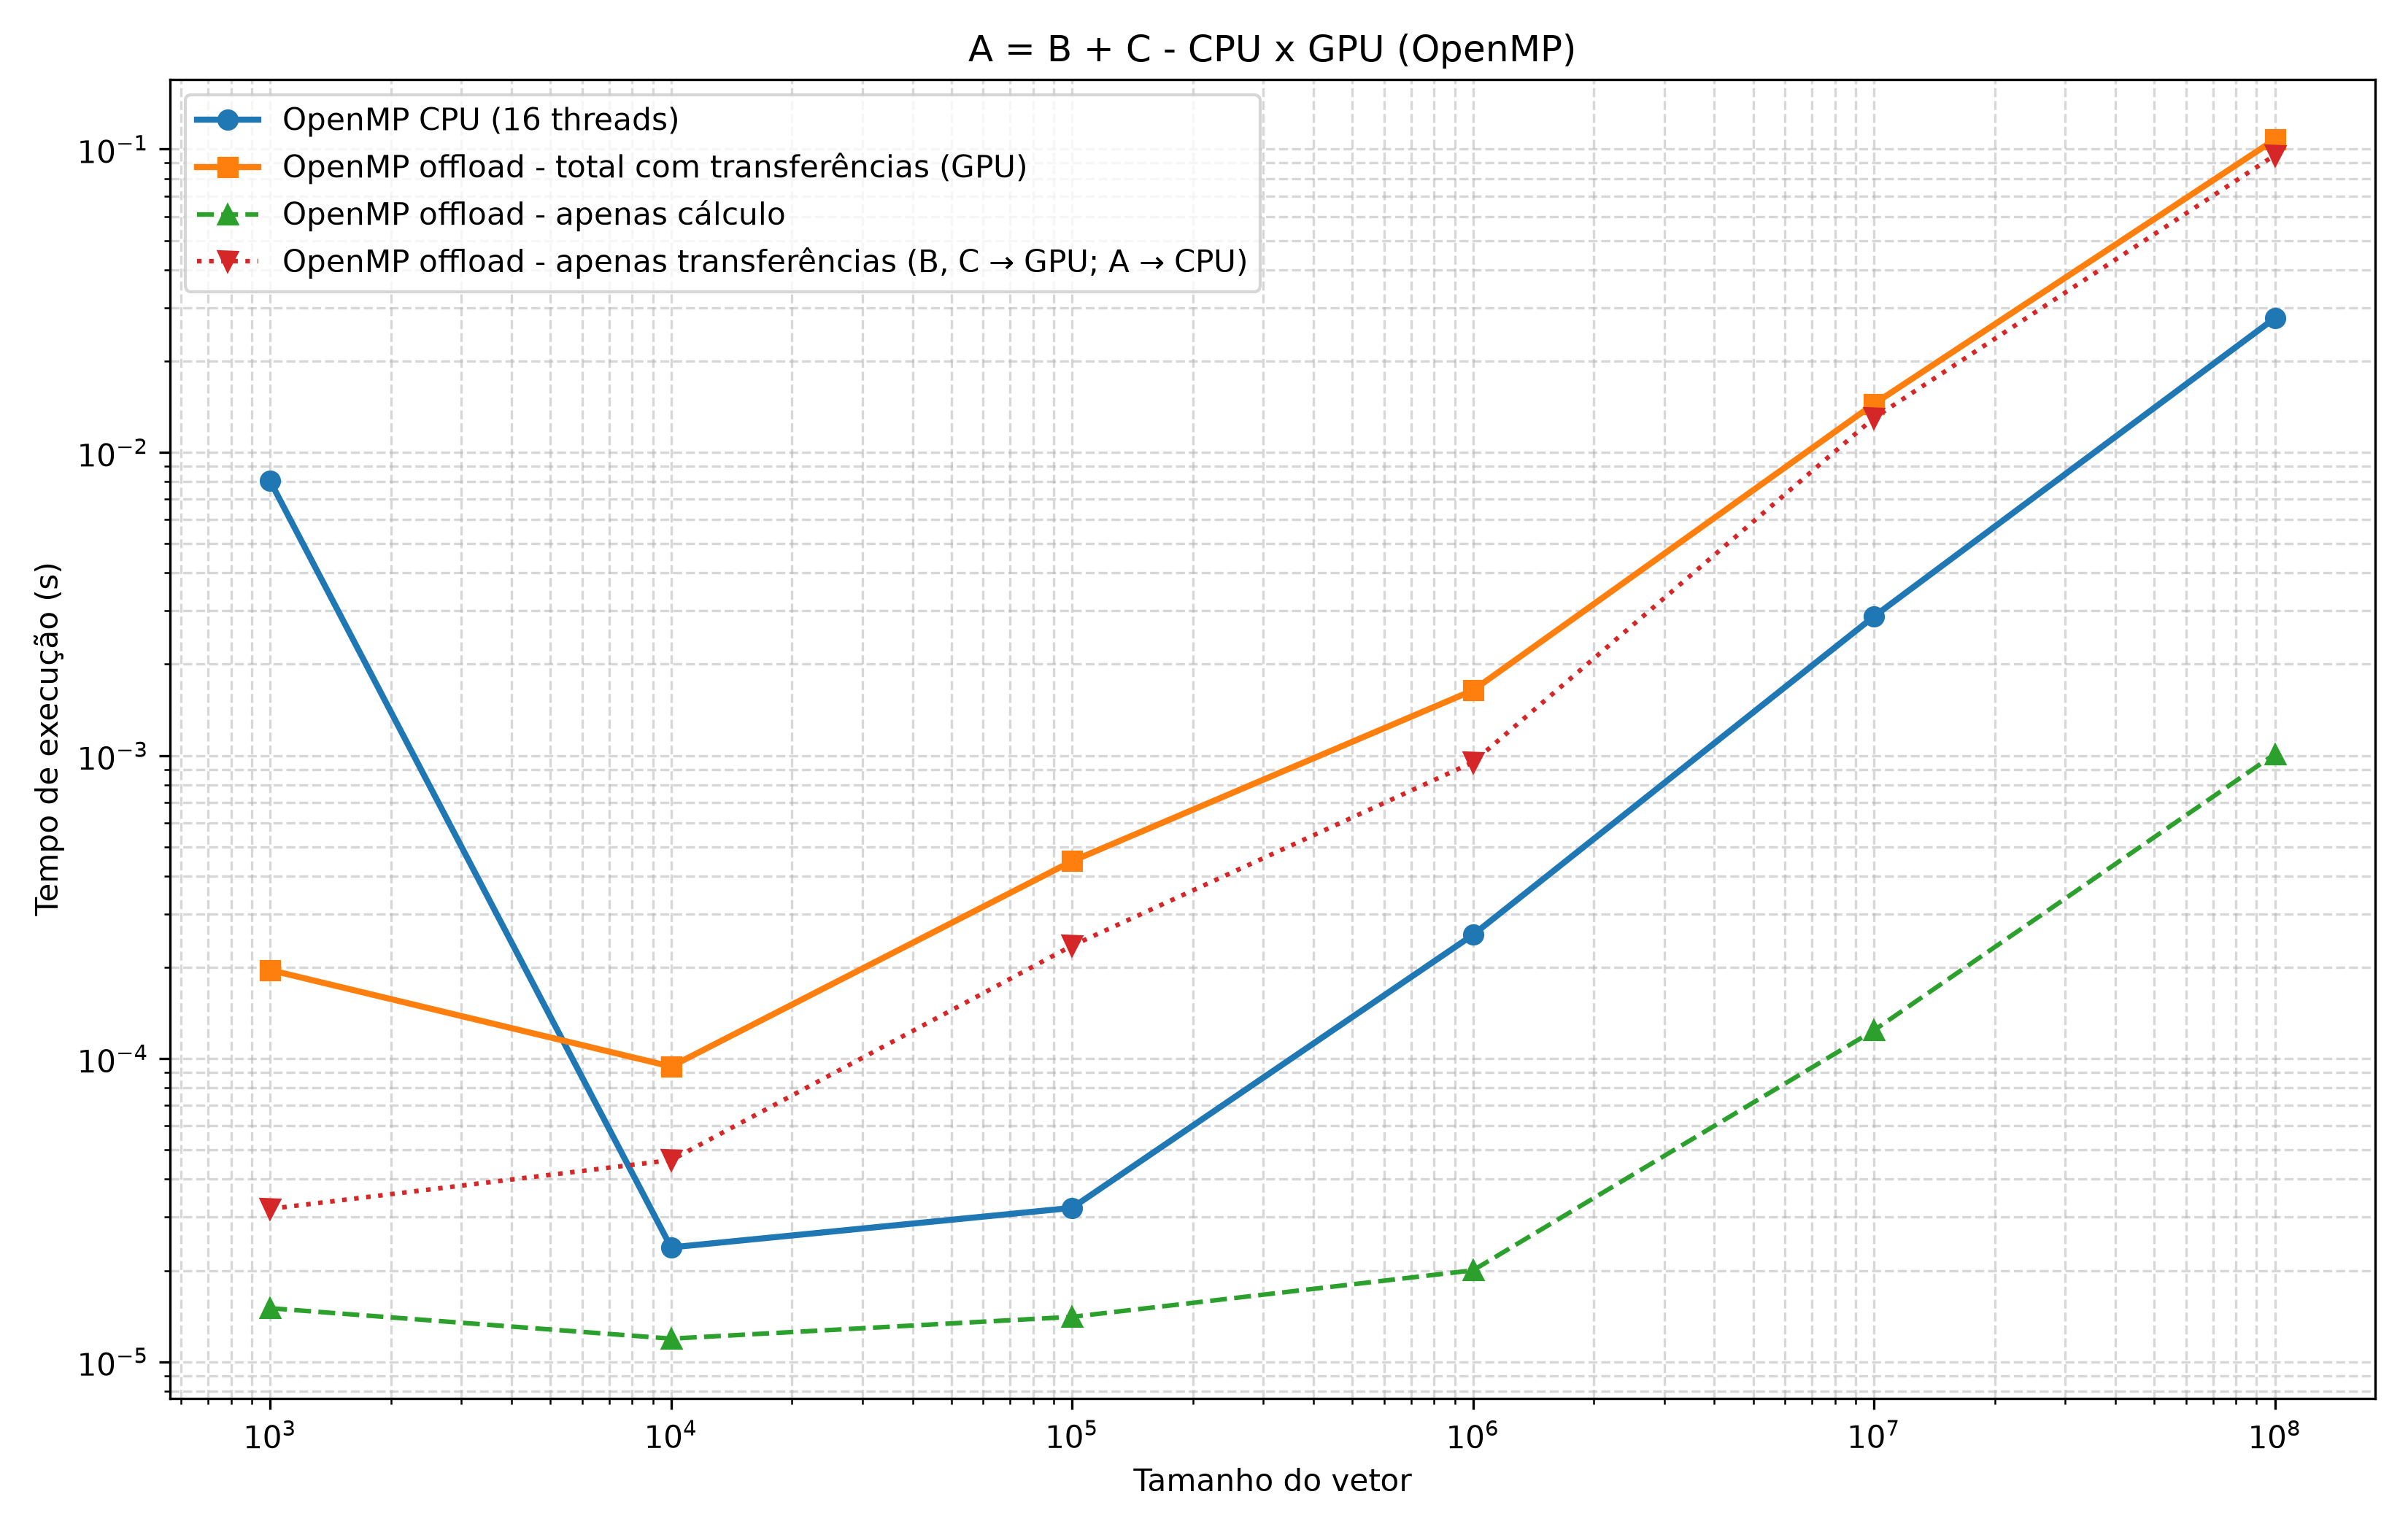
\includegraphics[width=\linewidth]{Tarefa11/tarefa11_tempos.png}
				\end{figure}
				\begin{figure}[H]
					\centering
					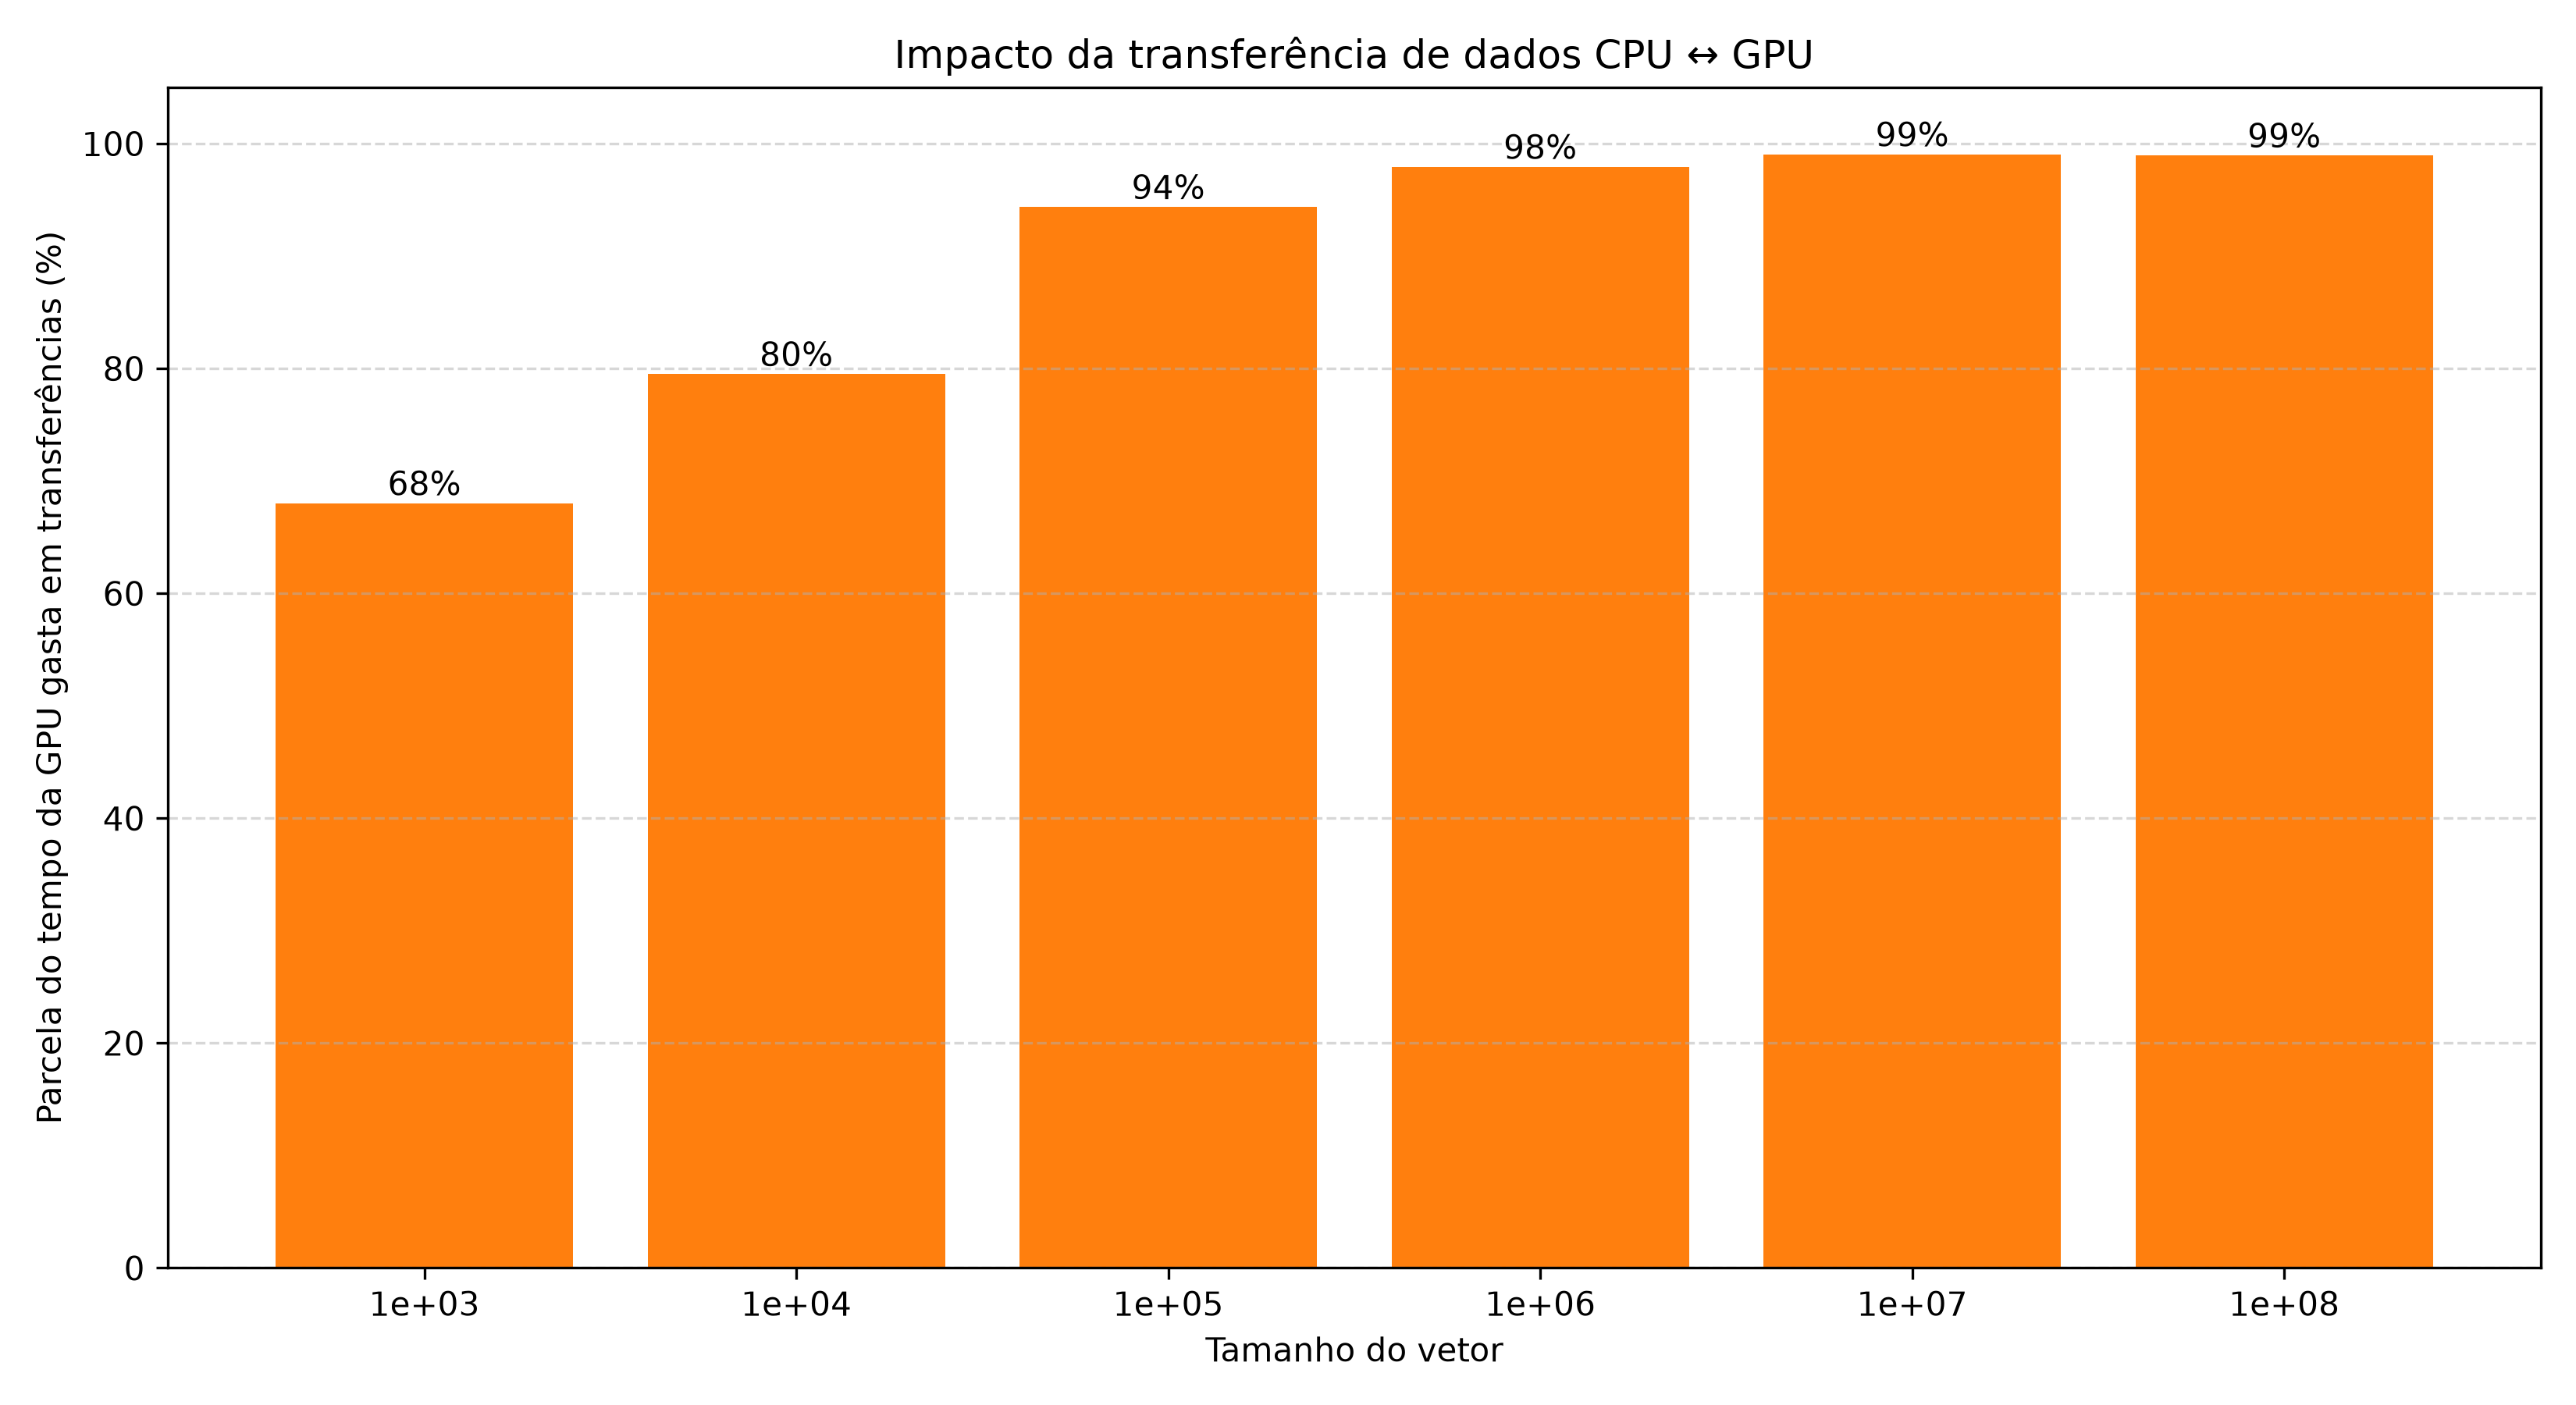
\includegraphics[width=\linewidth]{Tarefa11/tarefa11_transferencia.png}
				\end{figure}
				\par{Analisando os dados obtidos (gerados a partir da execução no supercomputador NPAD) mostrados nos gráficos, é possível verificar que o tempo de cálculo é significativamente menor durante o cálculo com GPU. Porém, ao analisarmos todo o escopo da execução, vemos que a versão paralela em CPU com OpenMP possui melhores tempos para as quantidades analisadas. Isso é causado pelo alto custo da transferência de dados entre os dispositivos, que faz com que a opção por GPU seja uma alternativa menos performática, apesar de um cálculo mais rápido.
				
				Pode-se verificar no gráfico um valor que foge do padrão apresentado durante os testes na primeira execução (o ponto mais à esquerda). Isso se deve provavelmente ao fato de ter sido justamente a primeira rodada de testes, e, portanto, os dispositivos estavam "frios". O código utilizado não considera rodadas de aquecimento, e por isso os primeiros cálculos podem apresentar certa ineficiência, como no caso verificado. }
			\subsection{\subtTres}
				\begin{lstlisting}[language=c]
				\end{lstlisting}

	\newpage
		\onehalfspacing
		\section{TAREFA 12}
		\subsection{\subtUm}
		\par{Texto}
		\subsection{\subtDois}
		\begin{figure}[H]
			\centering
			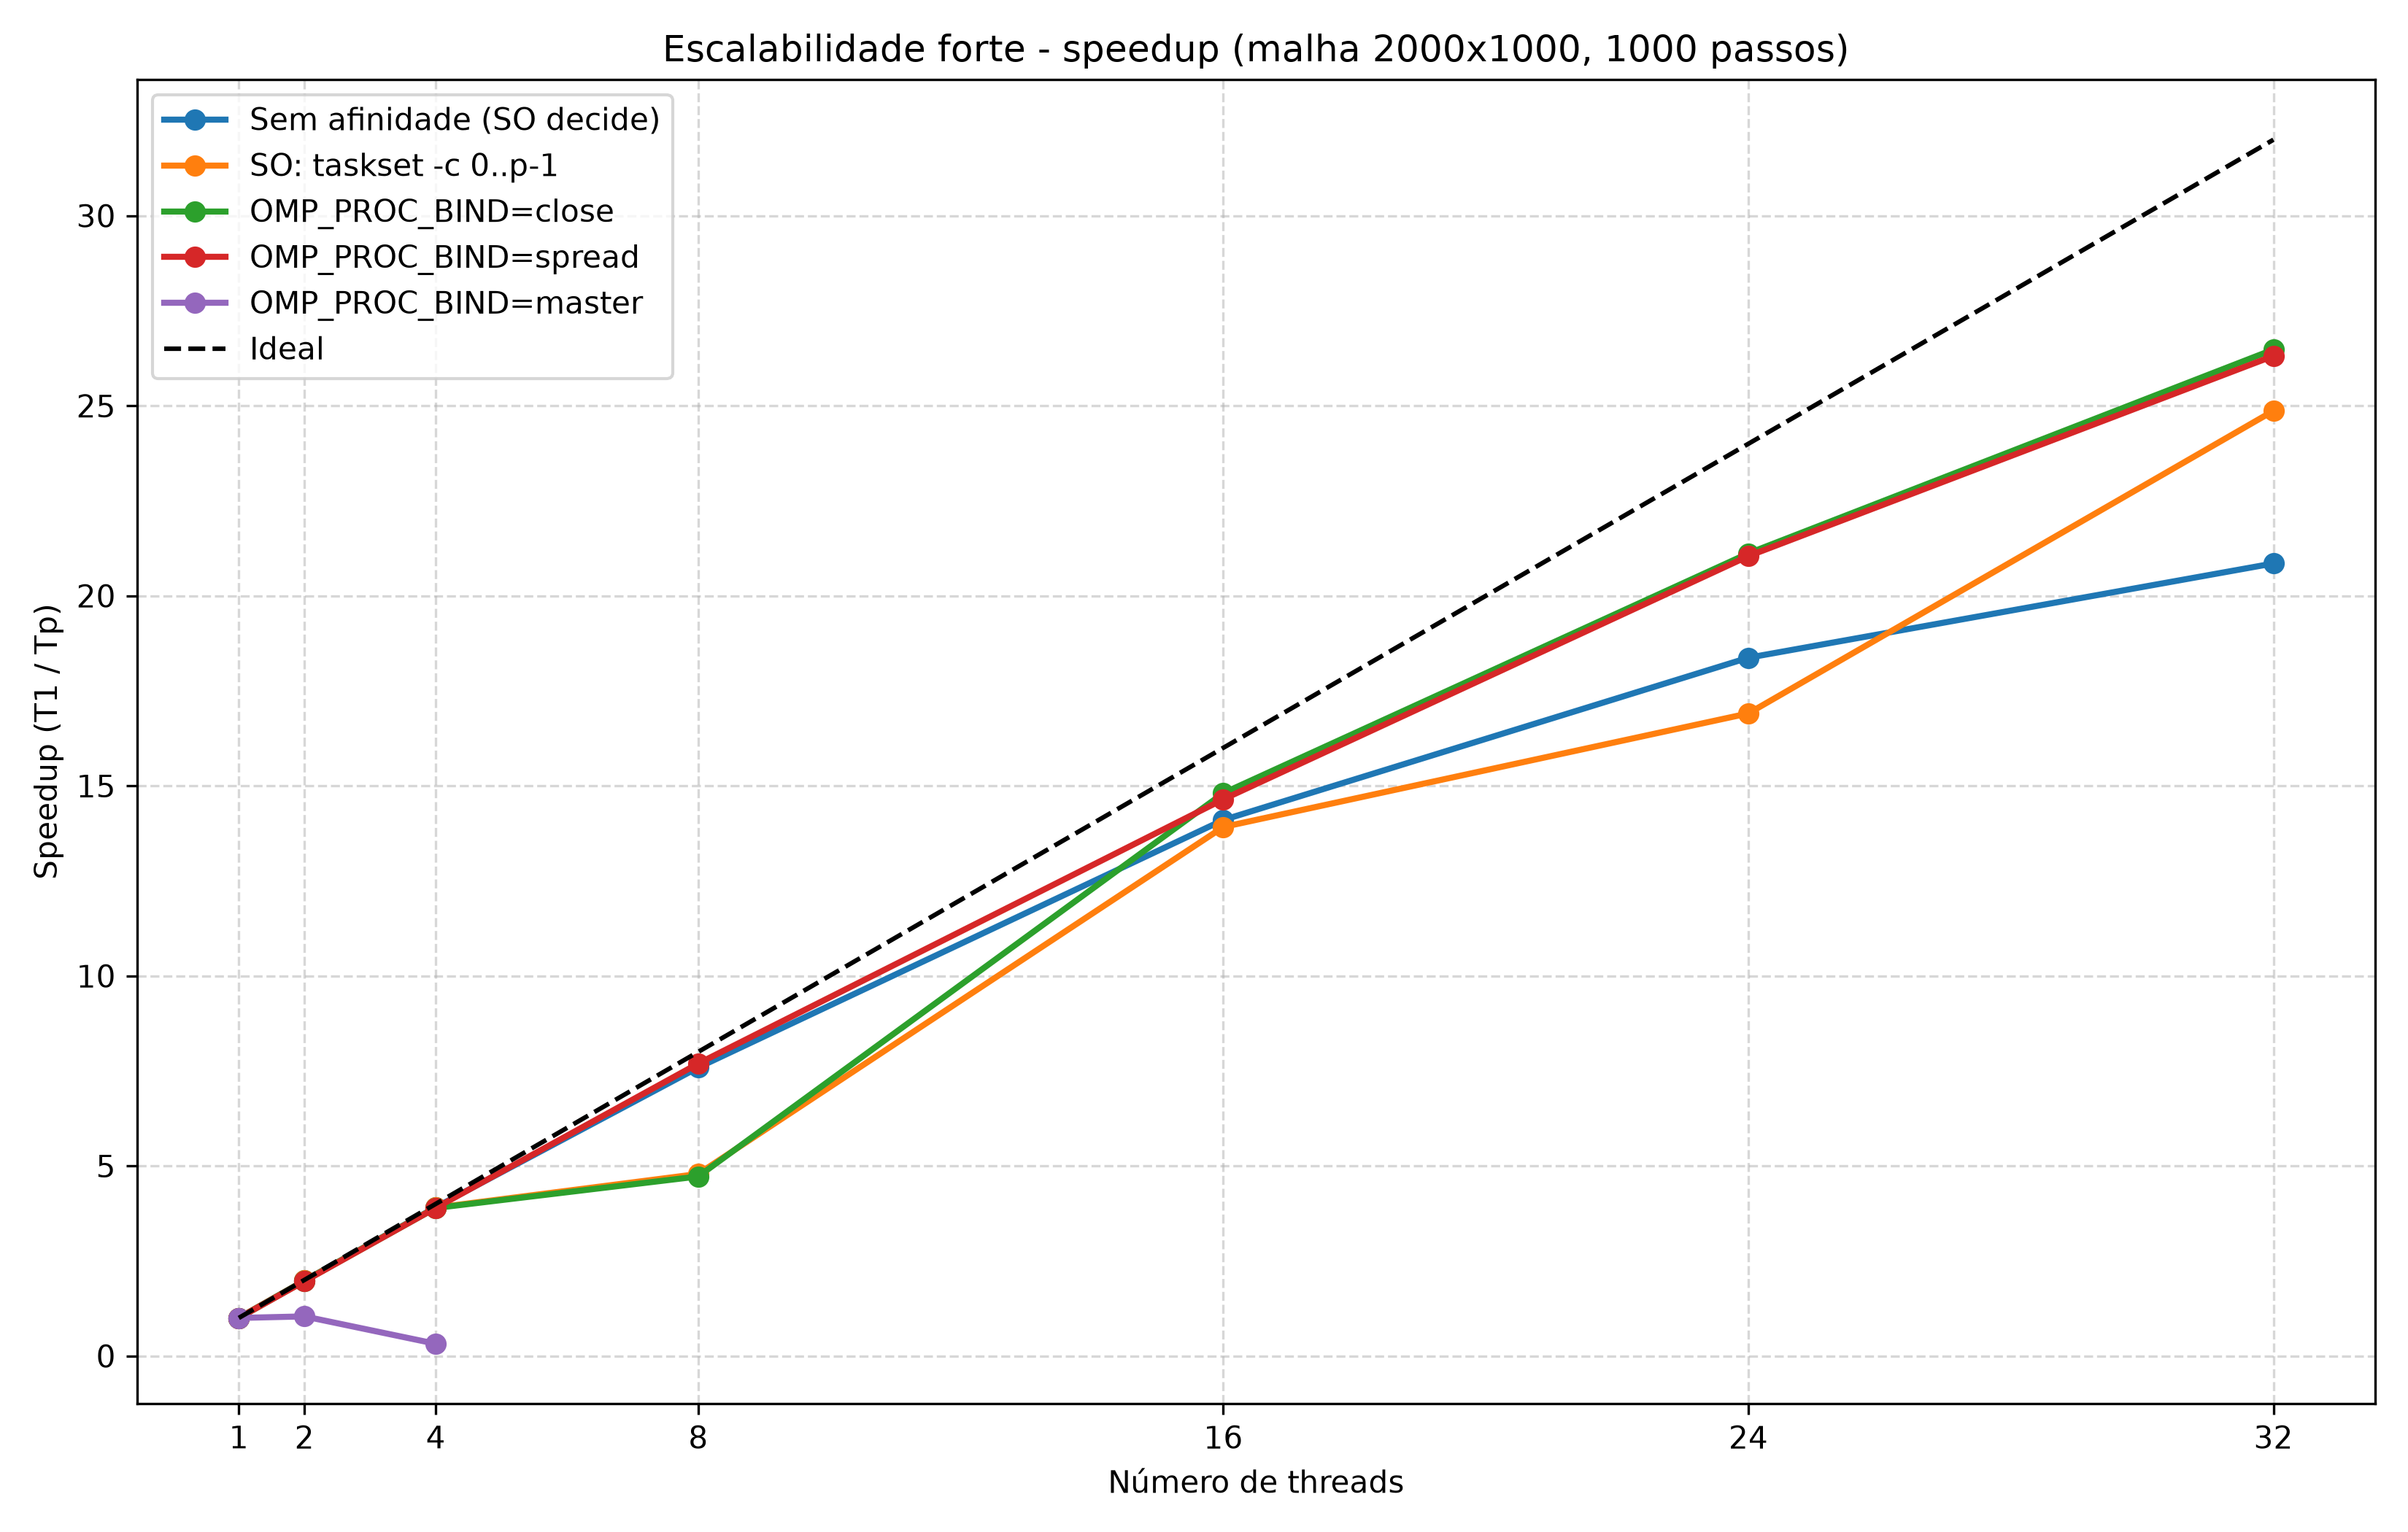
\includegraphics[width=\linewidth]{Tarefa12/tarefa12_speedup.png}
			\caption{Tarefa 12 -- Escalabilidade forte: \textit{speedup} ($T_1/T_p$) da propagação da onda com malha fixa, em função do número de threads, para cada política de afinidade (sem afinidade, \texttt{taskset}, \texttt{close}, \texttt{spread} e \texttt{master}).}
		\end{figure}
		\begin{figure}[H]
			\centering
			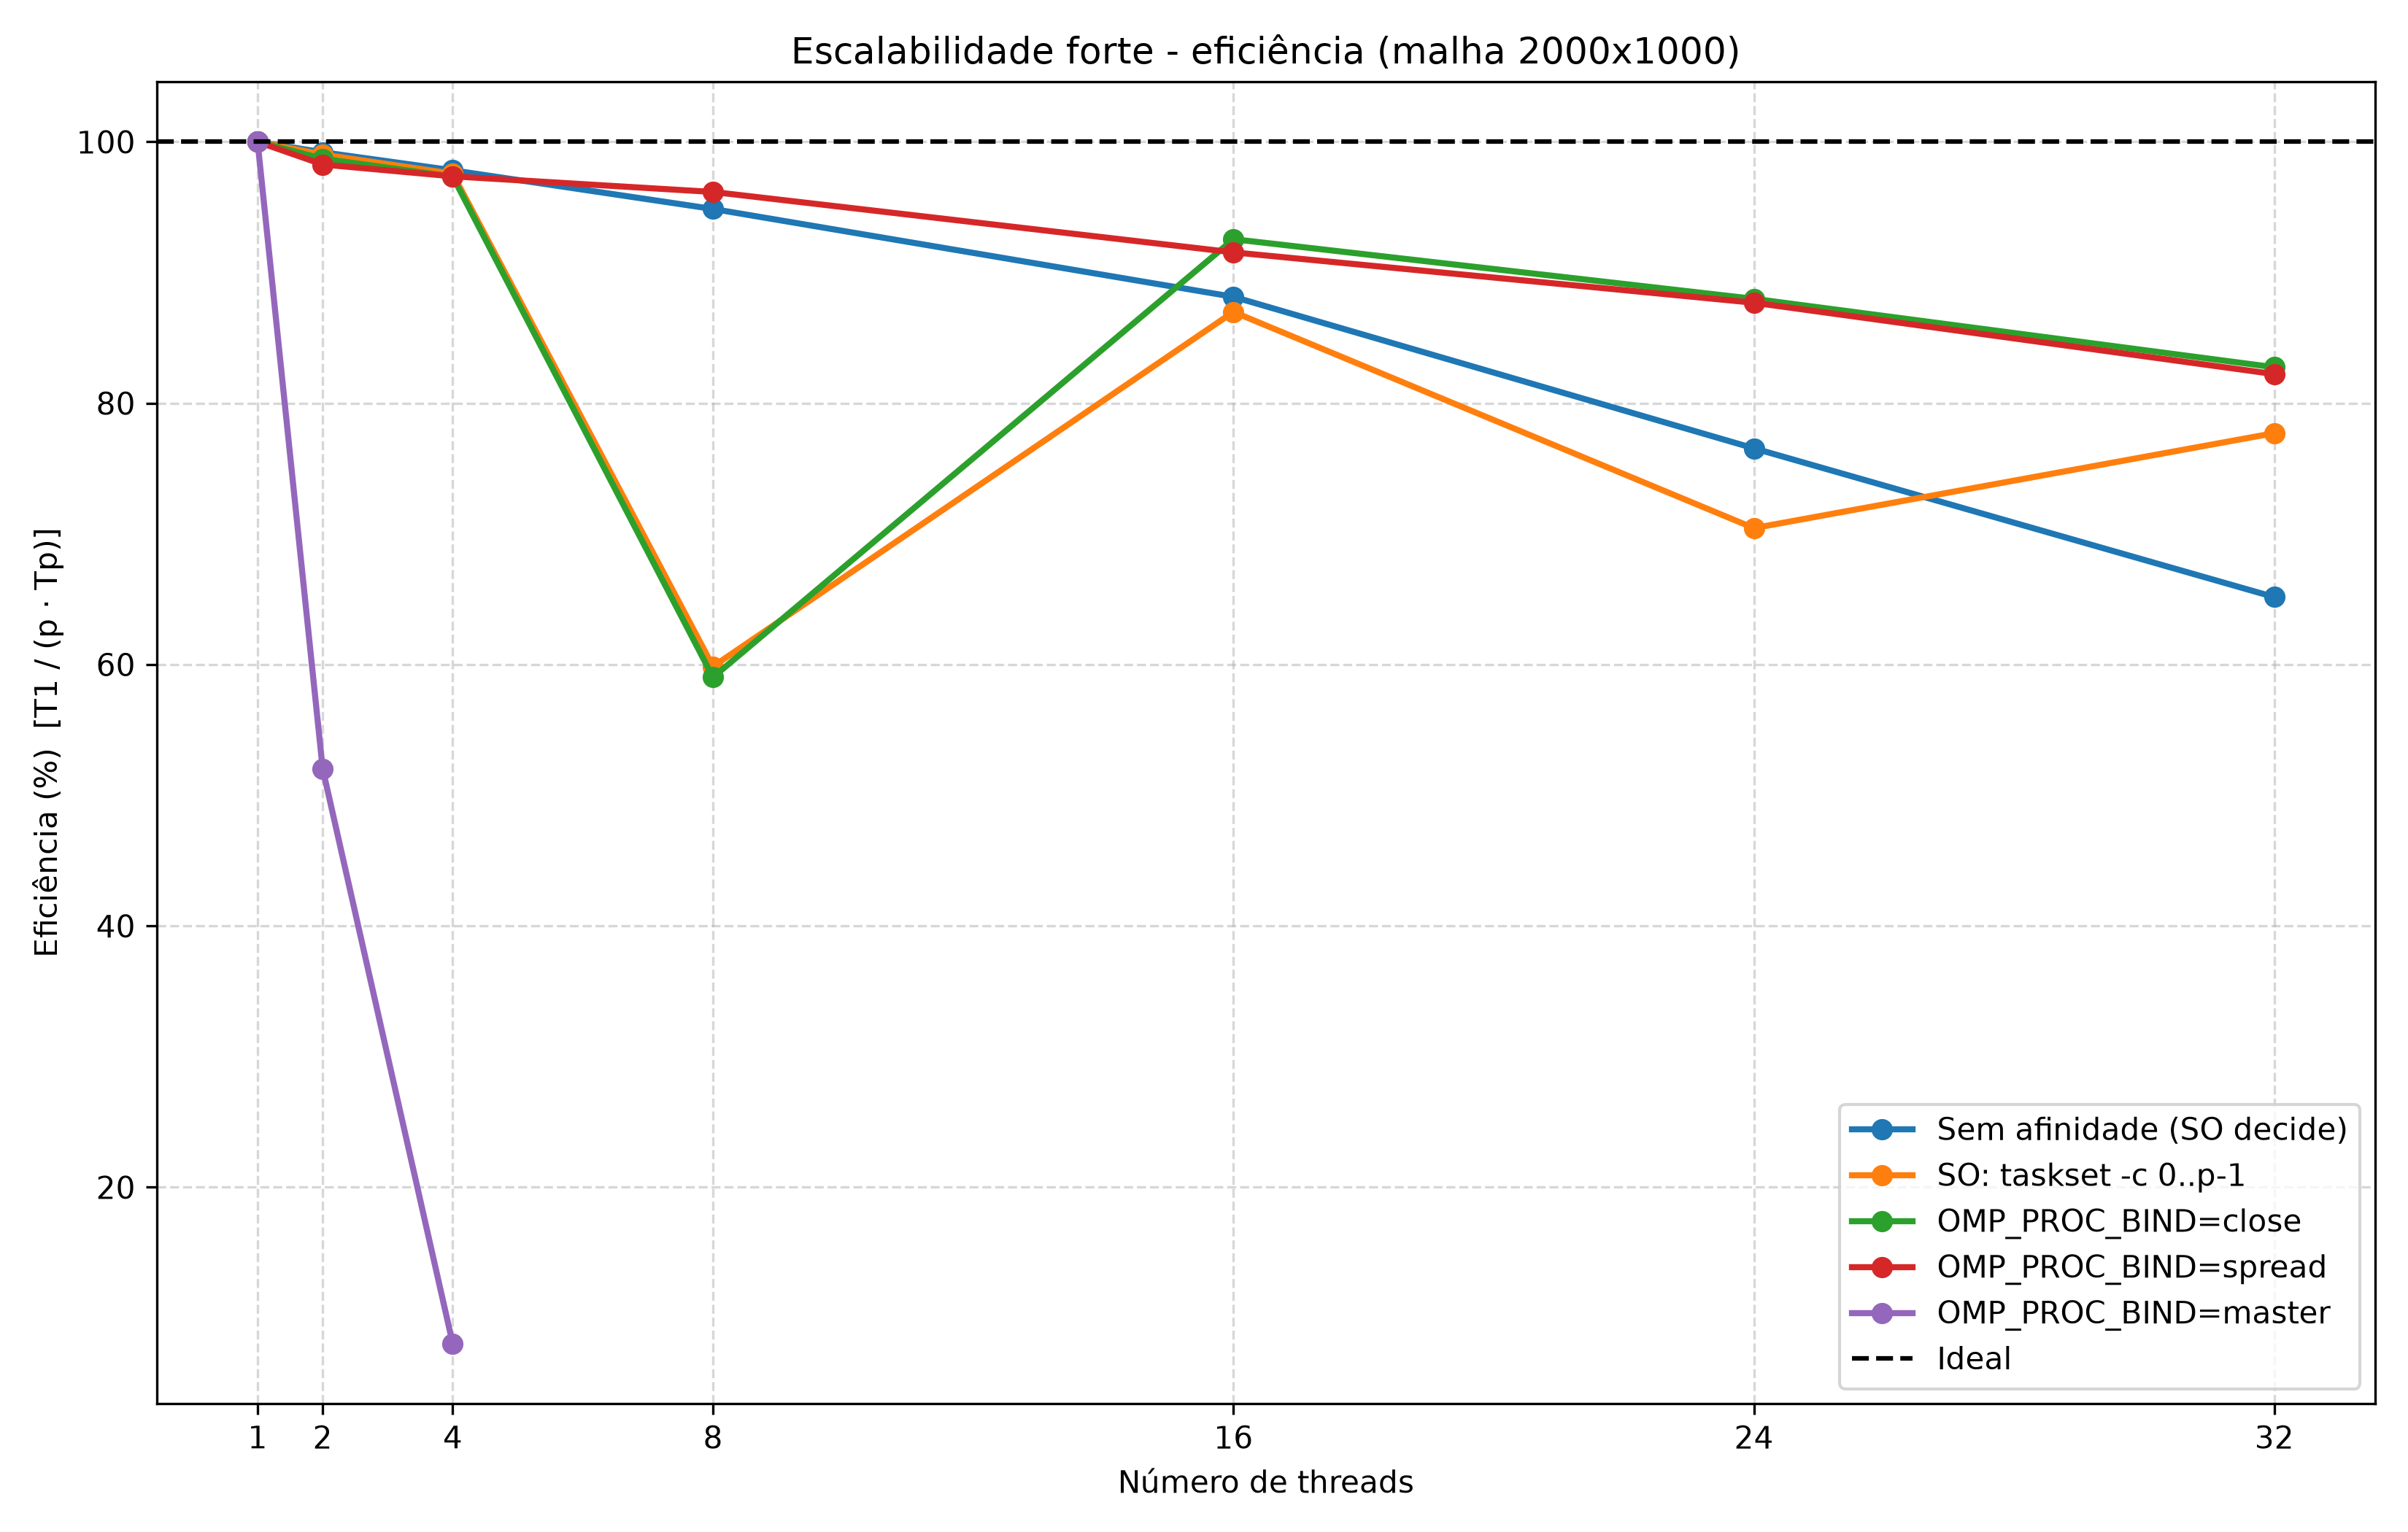
\includegraphics[width=\linewidth]{Tarefa12/tarefa12_eficiencia.png}
			\caption{Tarefa 12 -- Escalabilidade forte: eficiência paralela ($T_1/(p\,T_p)$) em função do número de threads para cada política de afinidade.}
		\end{figure}
		\begin{figure}
			\centering
			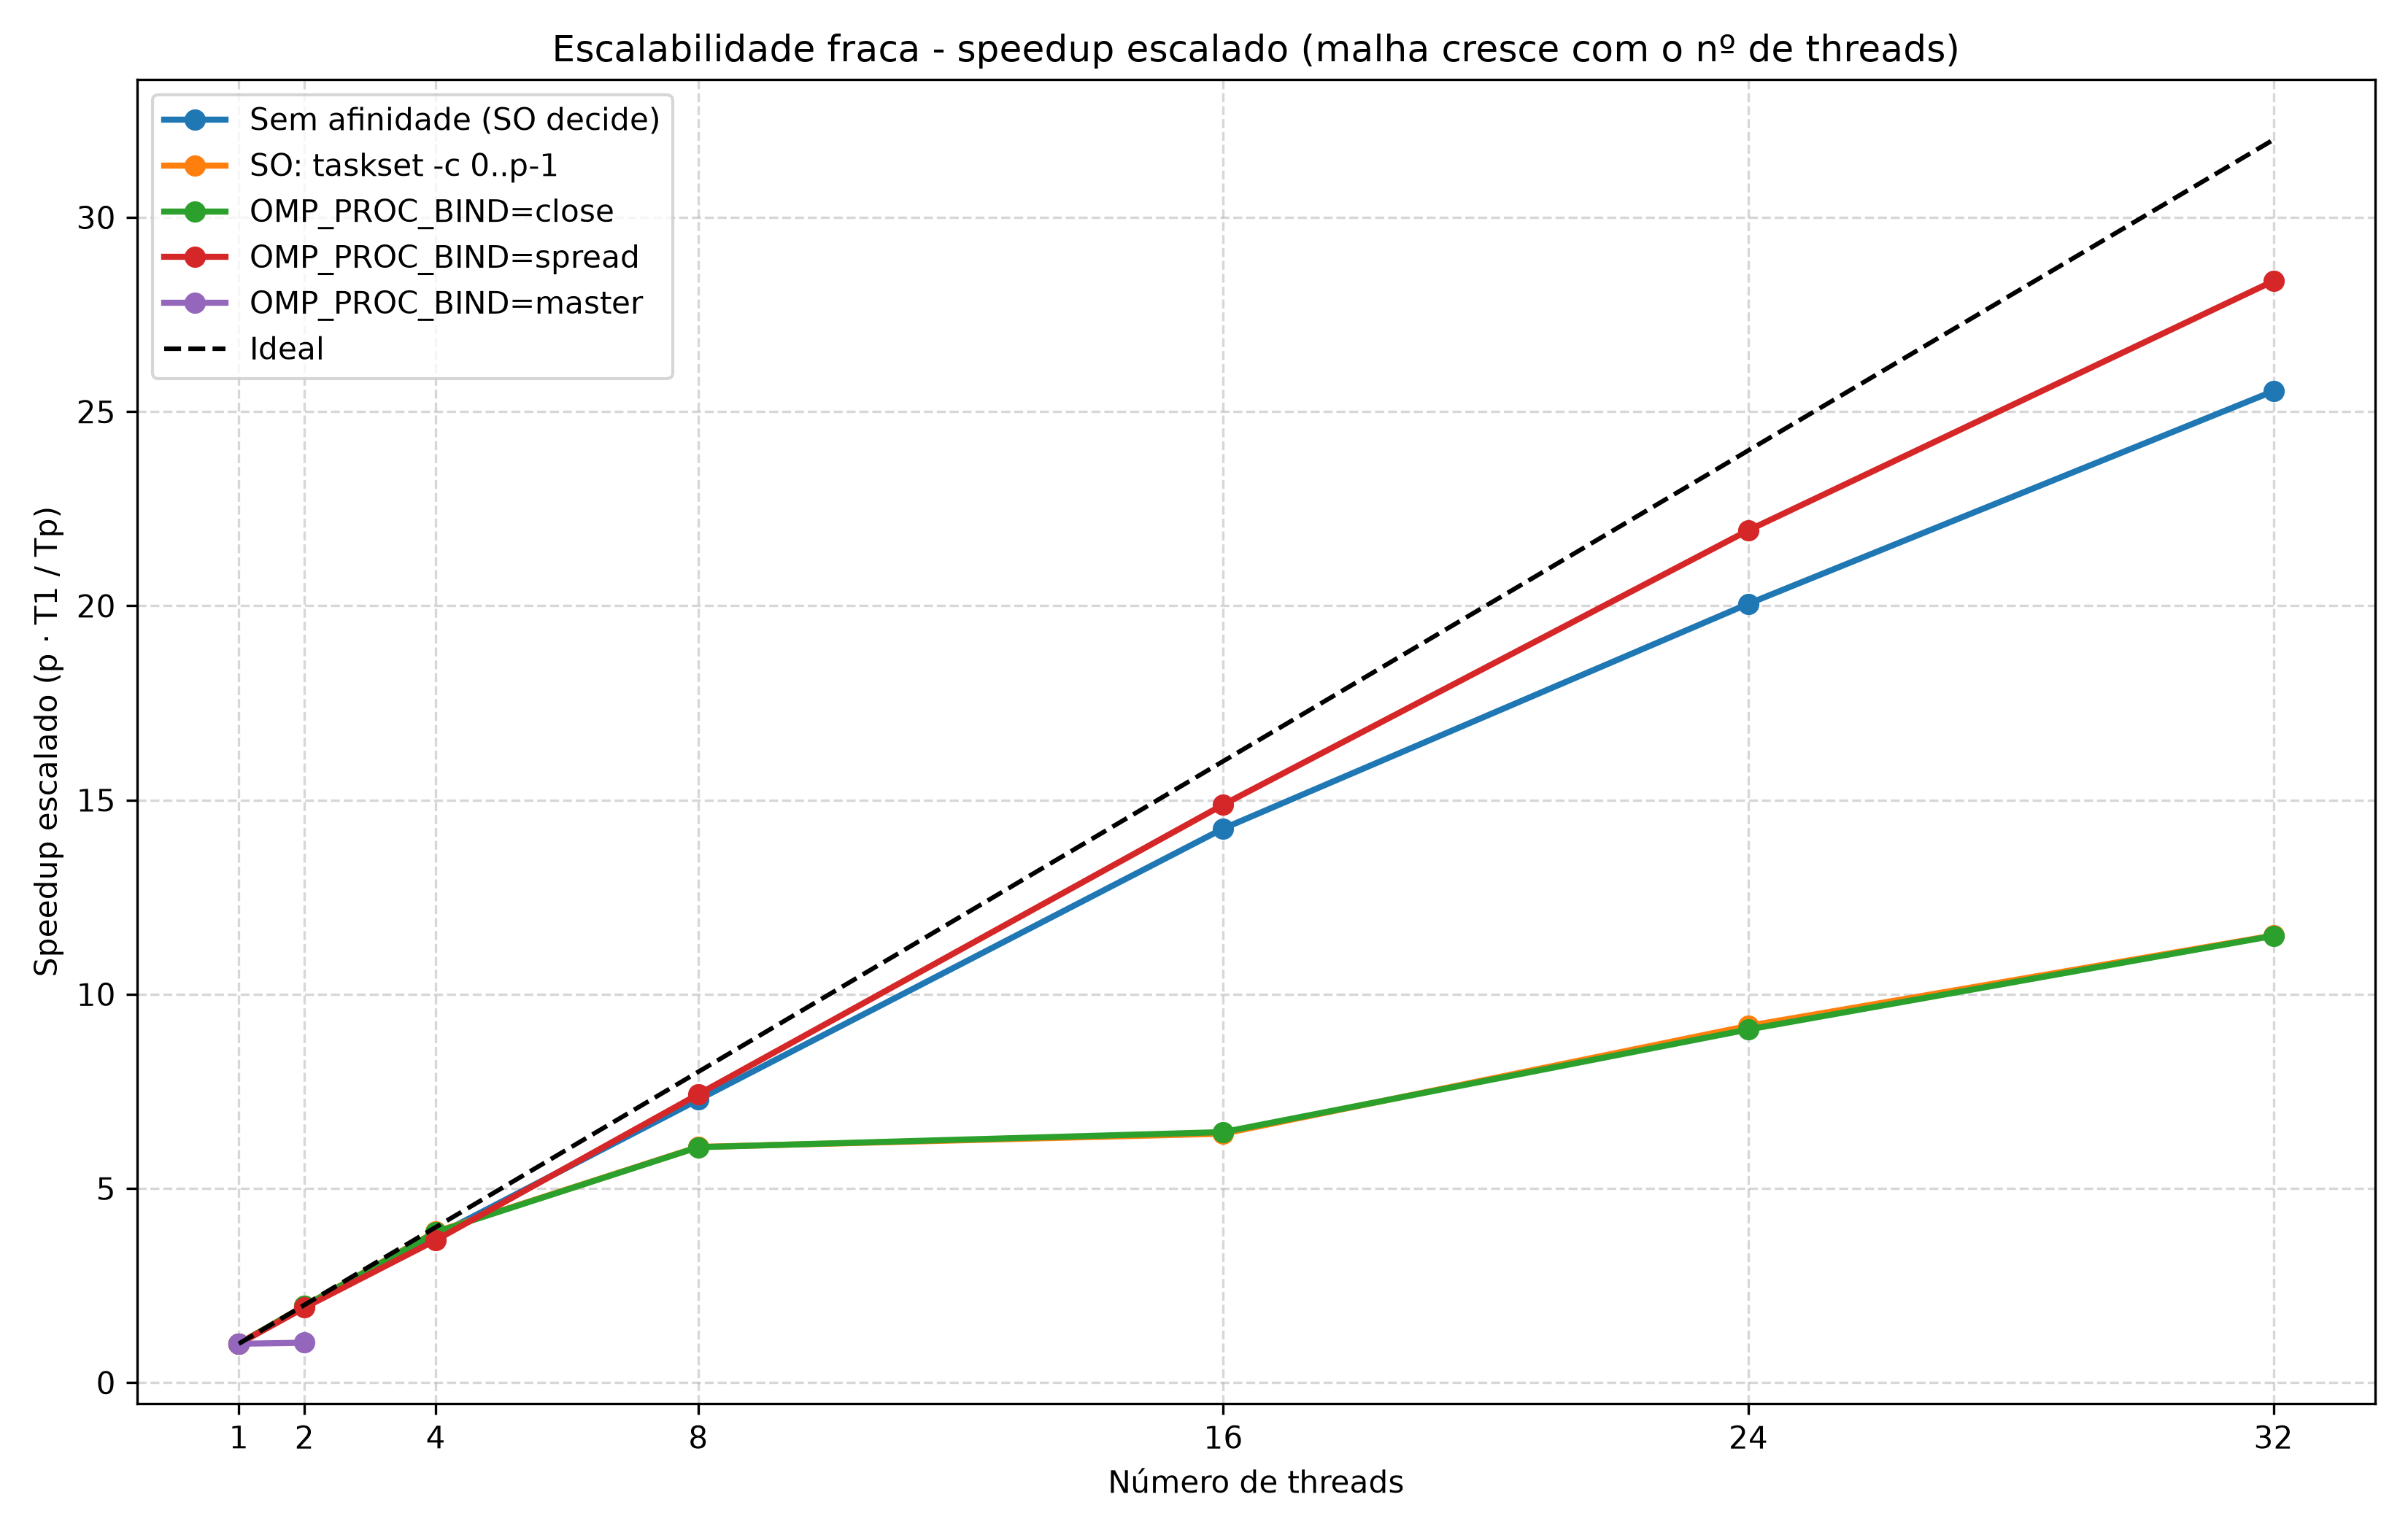
\includegraphics[width=\linewidth]{Tarefa12/tarefa12_speedup_fraca.png}
		\end{figure}
		\begin{figure}[H]
			\centering
			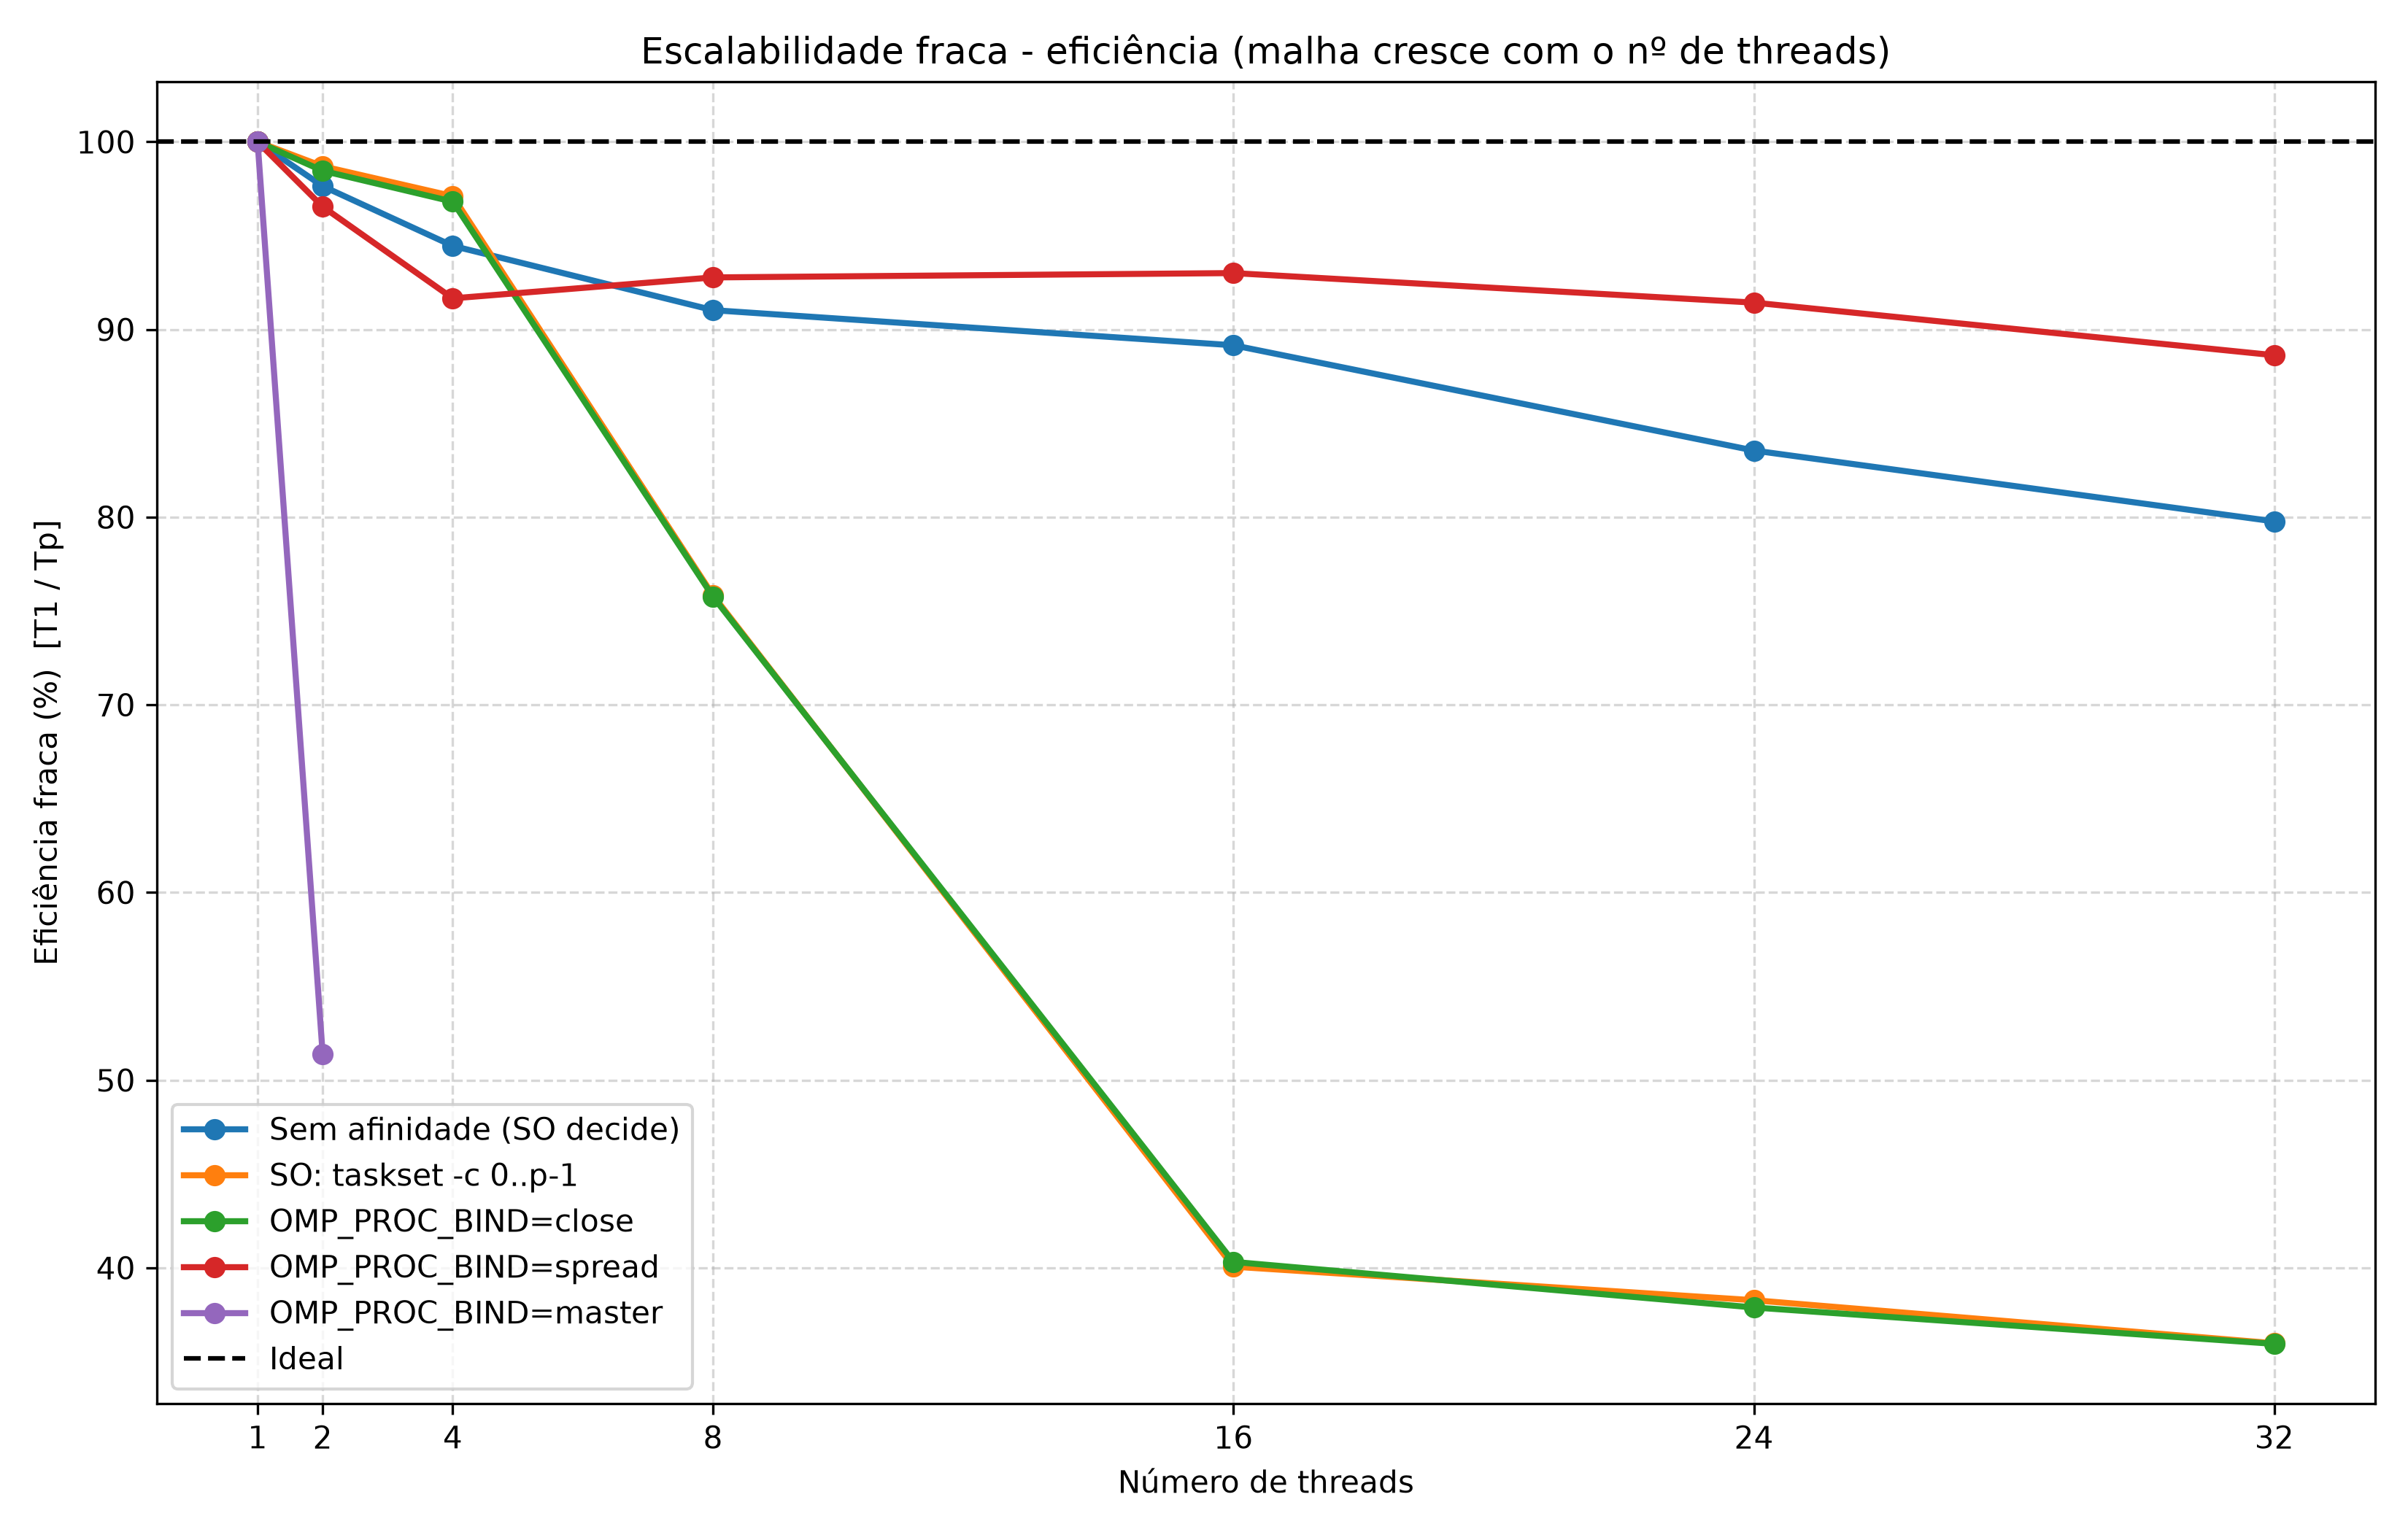
\includegraphics[width=\linewidth]{Tarefa12/tarefa12_fraca.png}
			\caption{Tarefa 12 -- Escalabilidade fraca: eficiência ($T_1/T_p$) com a malha crescendo proporcionalmente ao número de threads (mesma quantidade de trabalho por thread).}
		\end{figure}
		\begin{figure}[H]
			\centering
			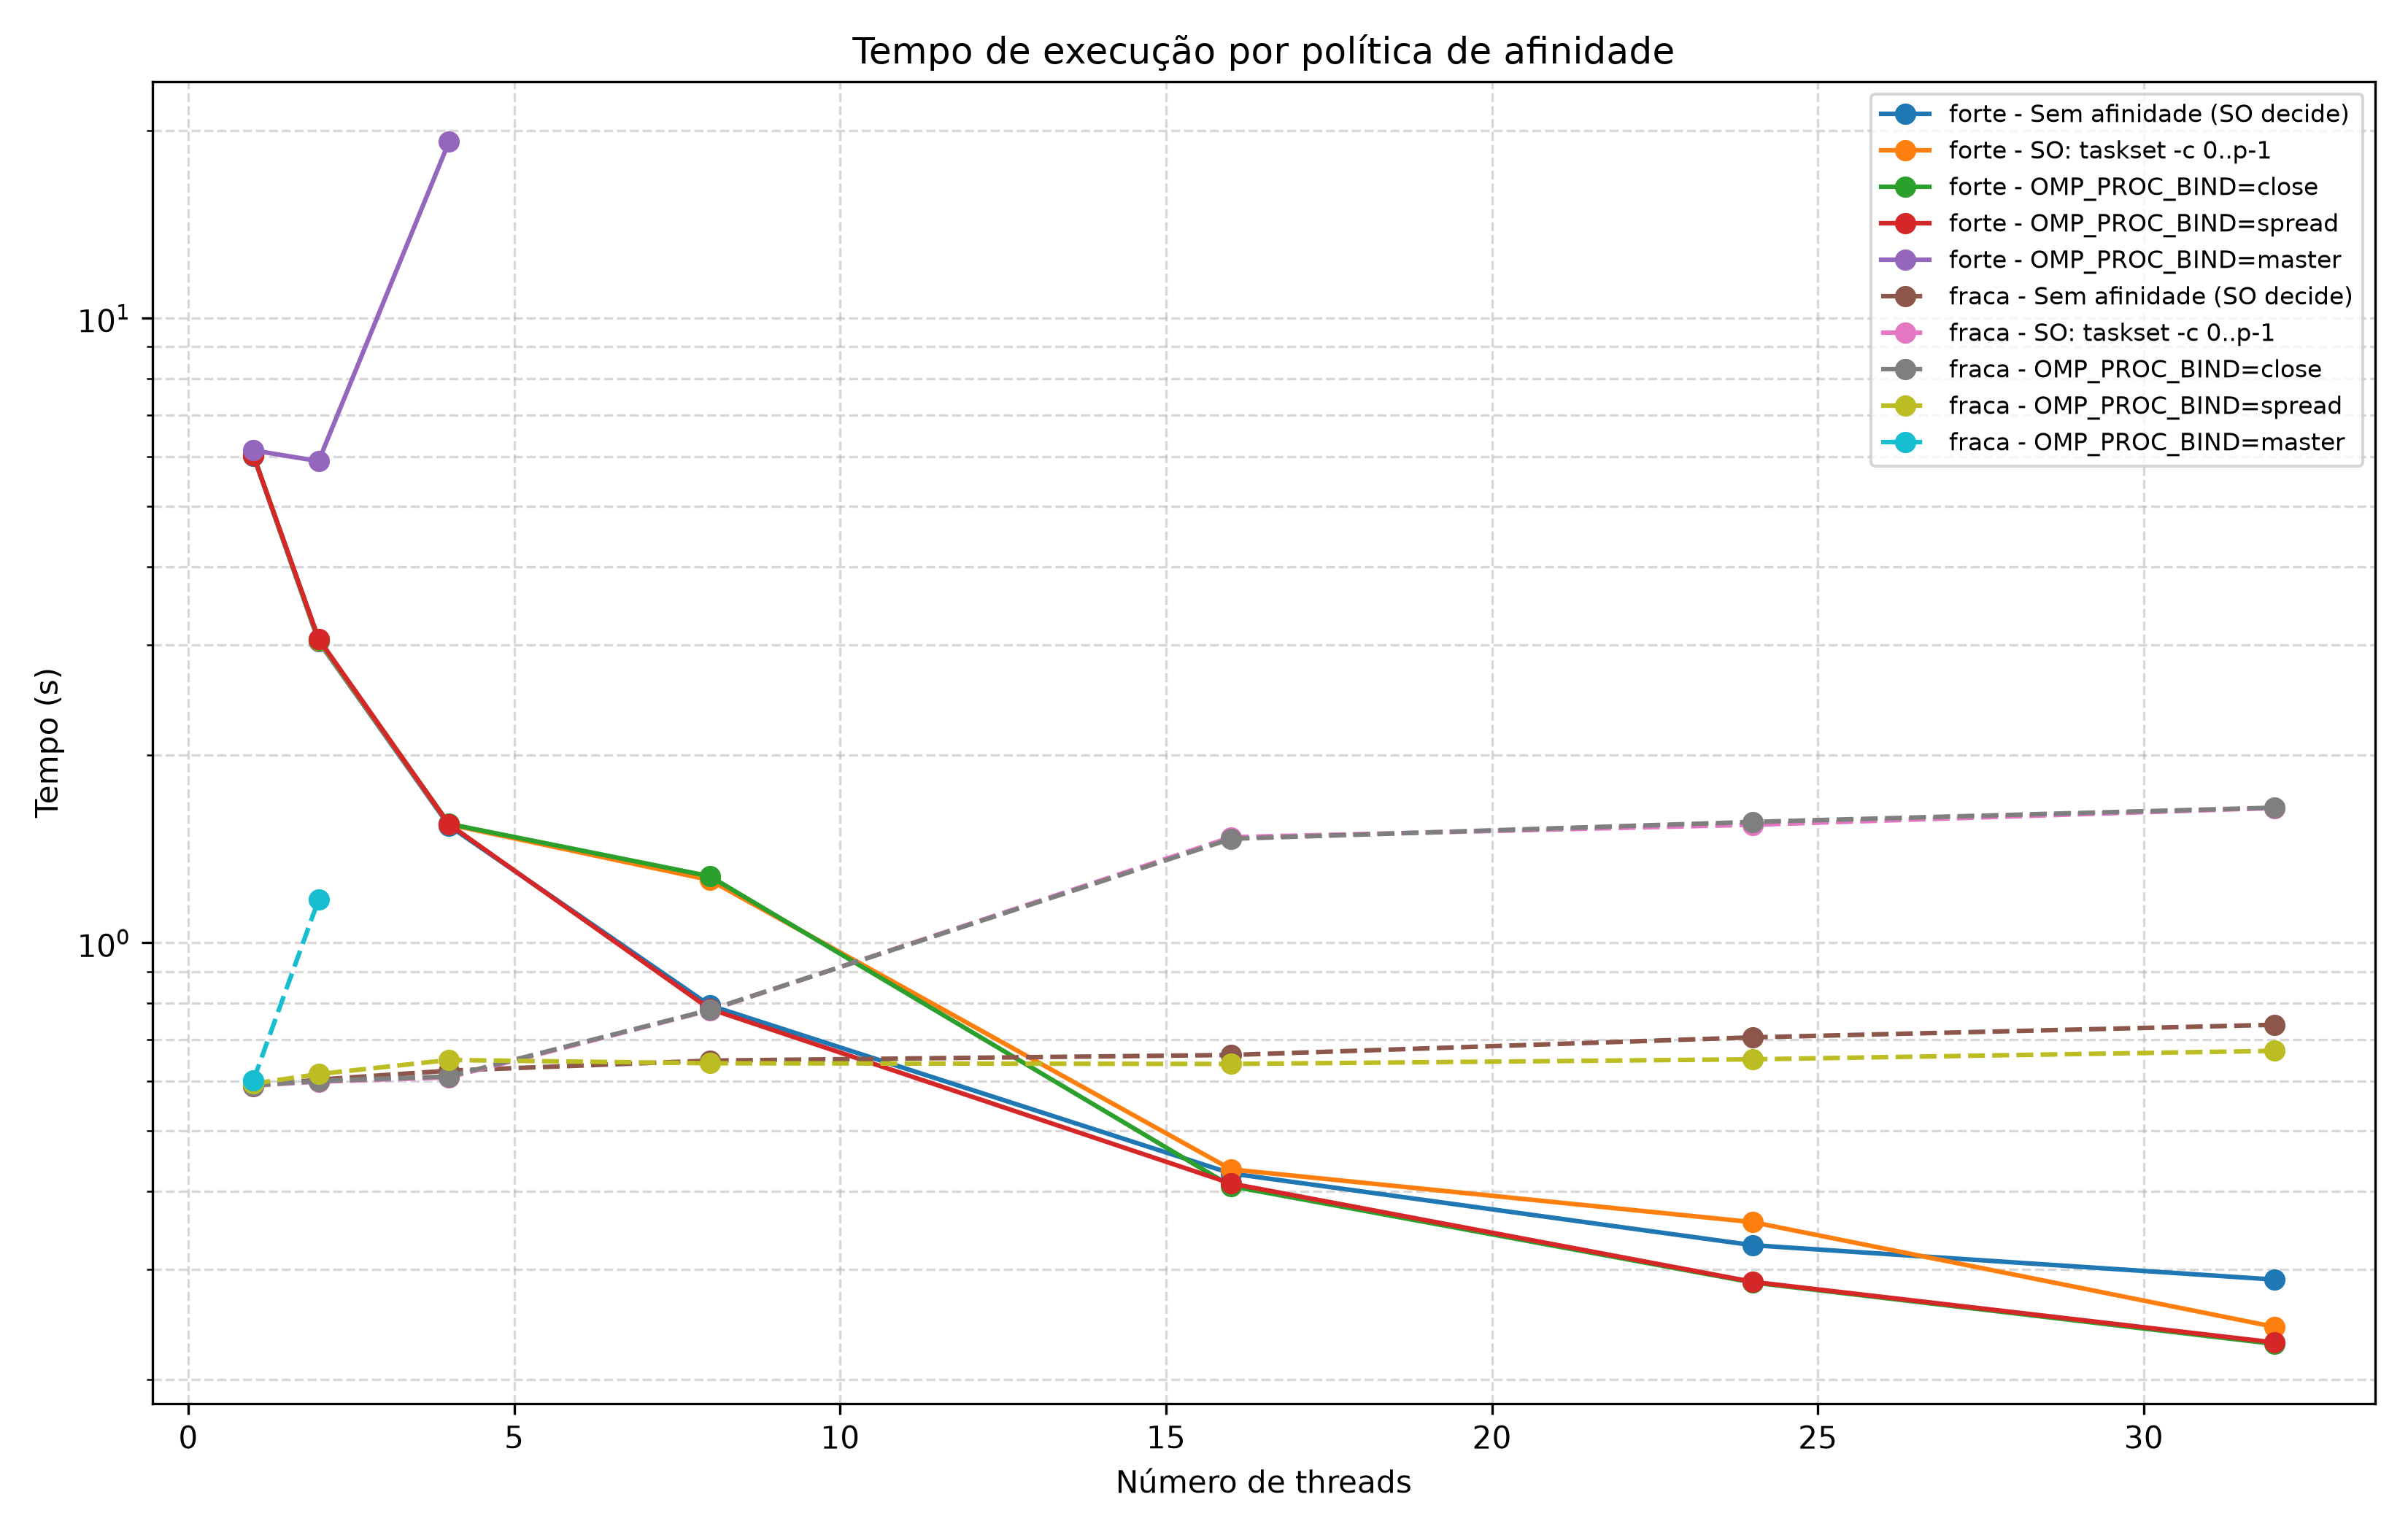
\includegraphics[width=\linewidth]{Tarefa12/tarefa12_tempos.png}
			\caption{Tarefa 12 -- Tempos de execução absolutos dos experimentos de escalabilidade forte (linha contínua) e fraca (linha tracejada) para cada política de afinidade.}
		\end{figure}
		\par{
				Analisando os dados e gráficos gerados, podemos notar alguns pontos importantes. 
			
			O primeiro é que a política master teve performance consideravelmente pior do que as outras, chegando a um fator de speedup nulo. Além disso, seus fatores de escalabilidade e tempo de execução mostram que, para esse tipo de problema, não é uma opção viável.
			
			A opção sem escolha de afinidade se mostra mais próxima aos outros resultados, mas ainda inferior às outras opções, exceto quando se tratando de escalabilidade fraca, em que  perde somente para a afinidade spread. O contrário ocorre com a política close, que se mostra em par com a spread para os casos de escalabilidade forte, mas perde performance para escalabilidade fraca.
			
			Portanto, a melhor escolha para esse tipo de algorítmo é a política de afinidade spread, que apresenta os melhores números de desempenho em todos os casos analisados quando comparado às suas alternativas.
			}
		\subsection{\subtTres}
		\begin{lstlisting}[language=c]
		\end{lstlisting}
		
	\newpage
		\onehalfspacing
		\section{TAREFA 13}
		\subsection{\subtUm}
		\par{Texto}
		\subsection{\subtDois}
		
		\begin{figure}[H]
			\centering
			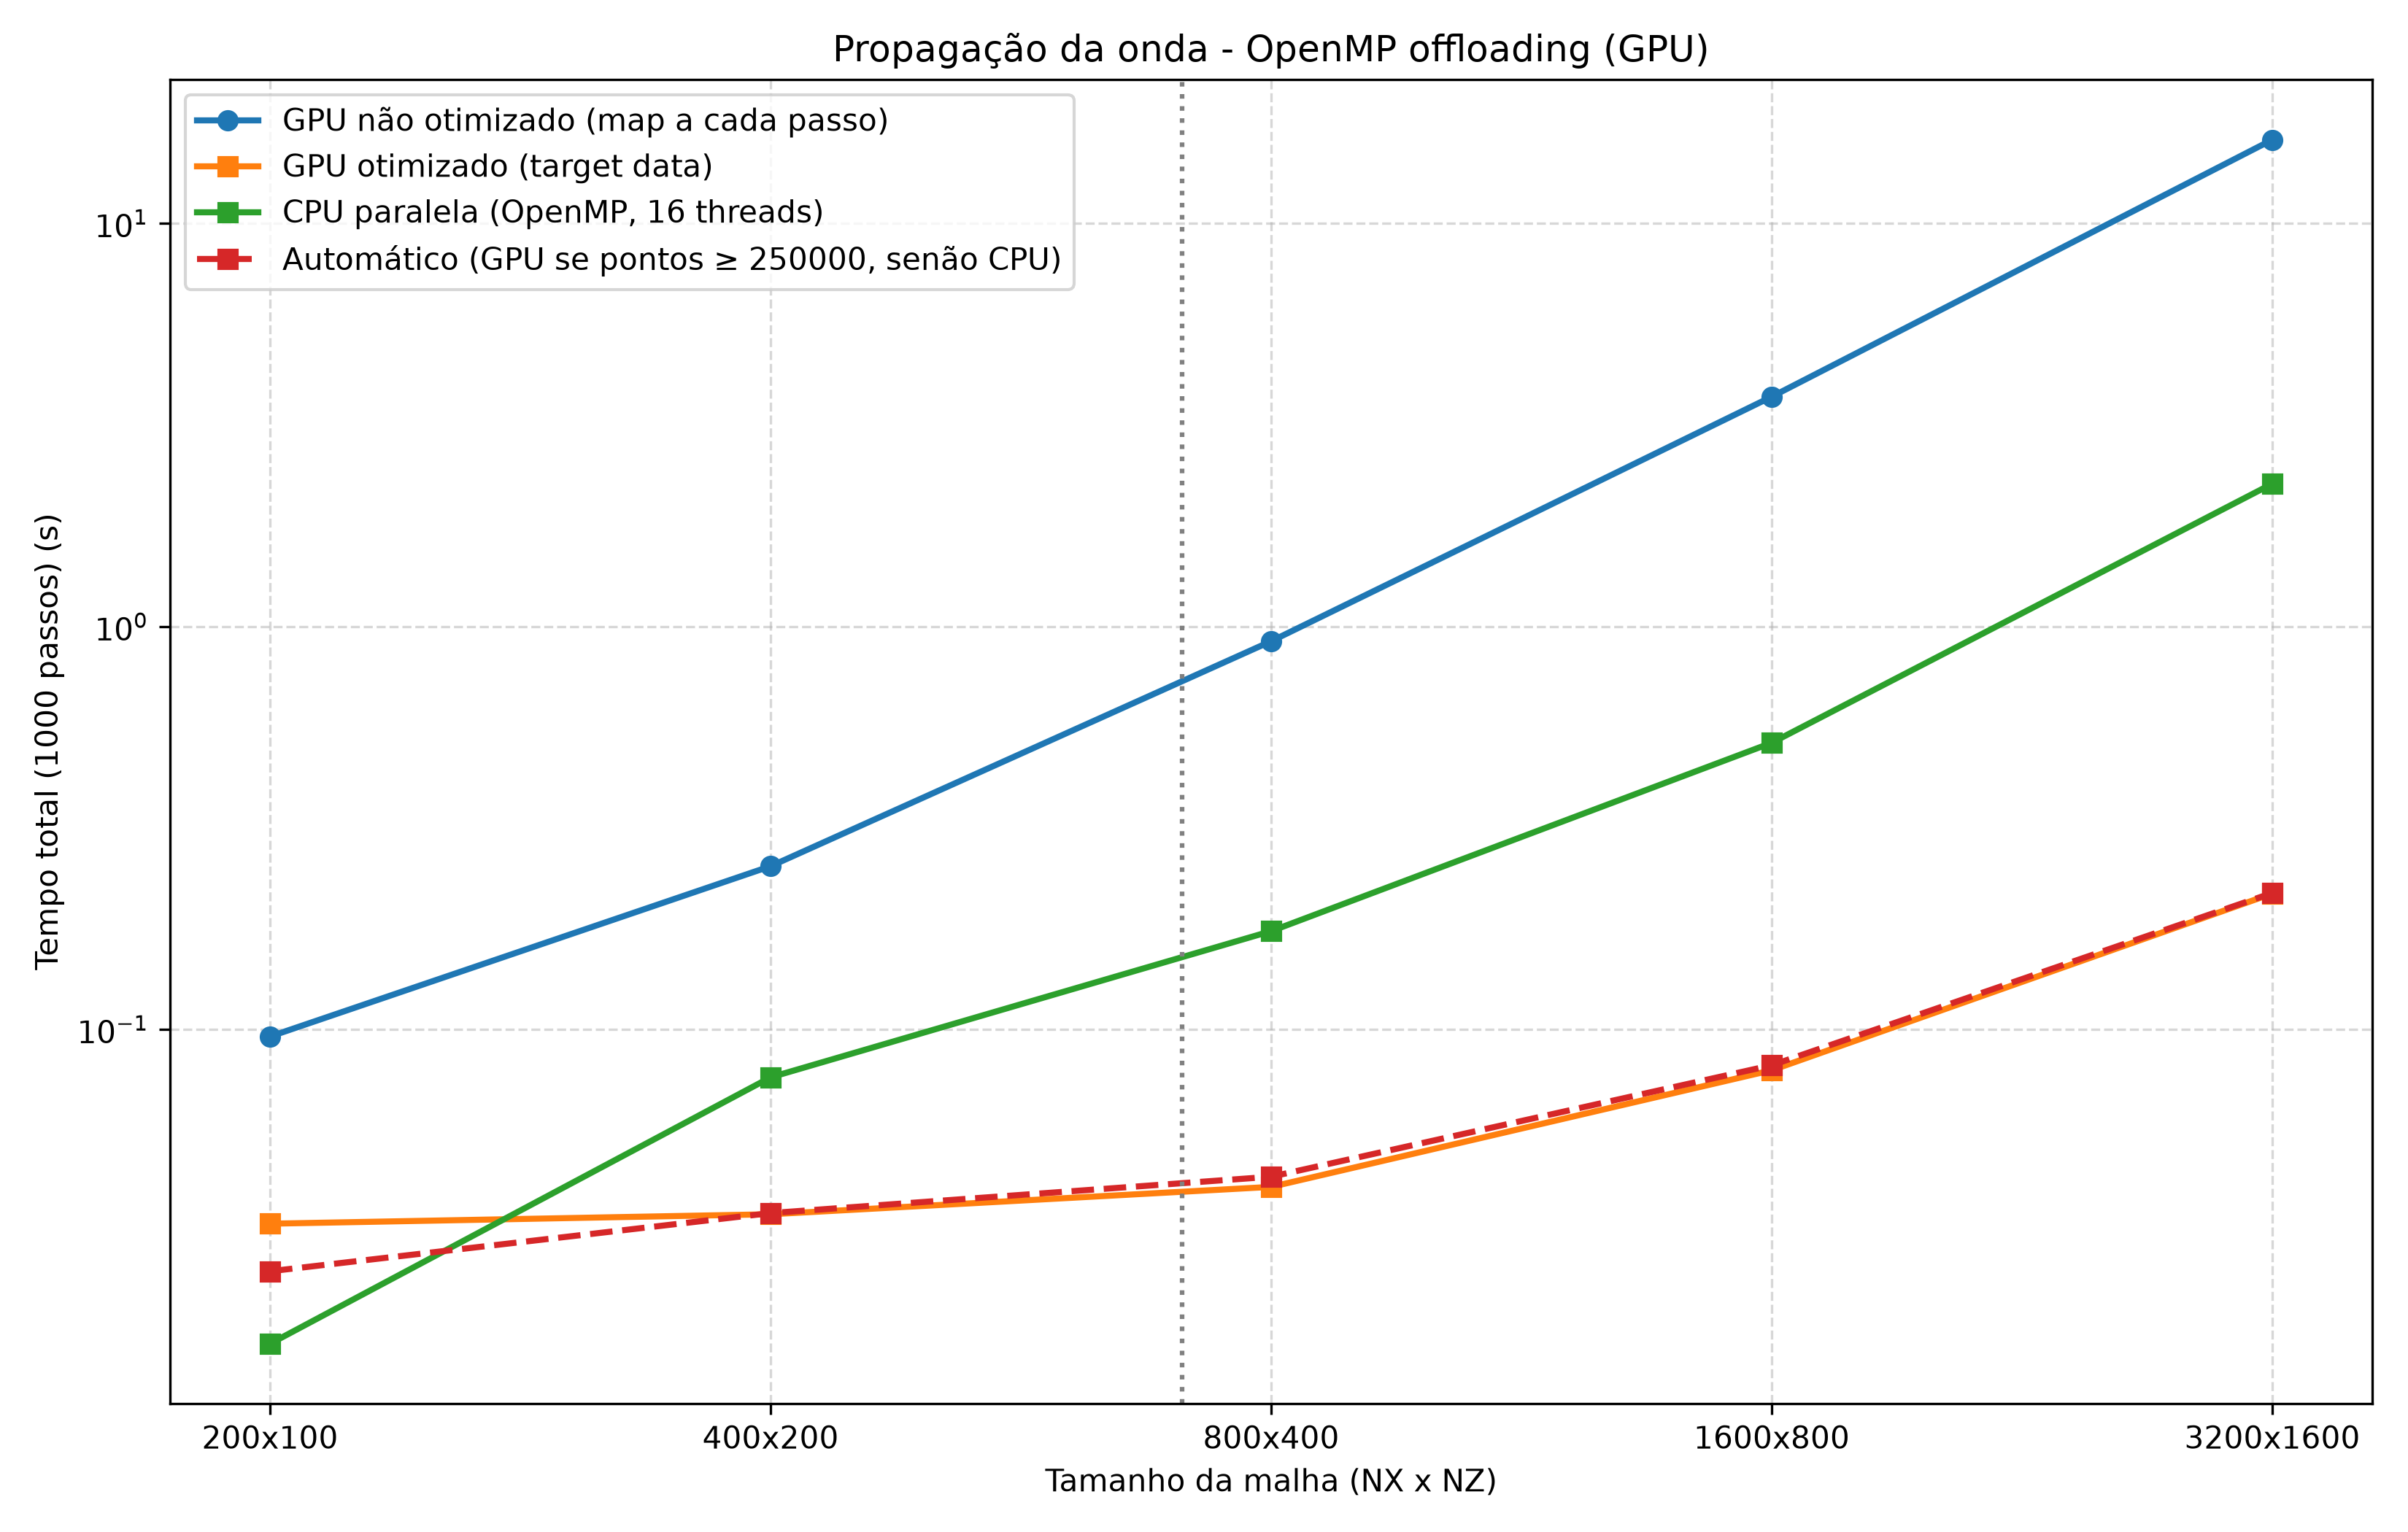
\includegraphics[width=\linewidth]{Tarefa13/tarefa13_tempos.png}
			\caption{Tarefa 13 -- Tempo total da propagação da onda (1000 passos) em função do tamanho da malha: versão não otimizada (\texttt{map} a cada passo), versão otimizada com \texttt{target data} sempre na GPU, sempre na CPU e com decisão automática pelo tamanho do problema (cláusula \texttt{if}).}
		\end{figure}
		\begin{figure}[H]
			\centering
			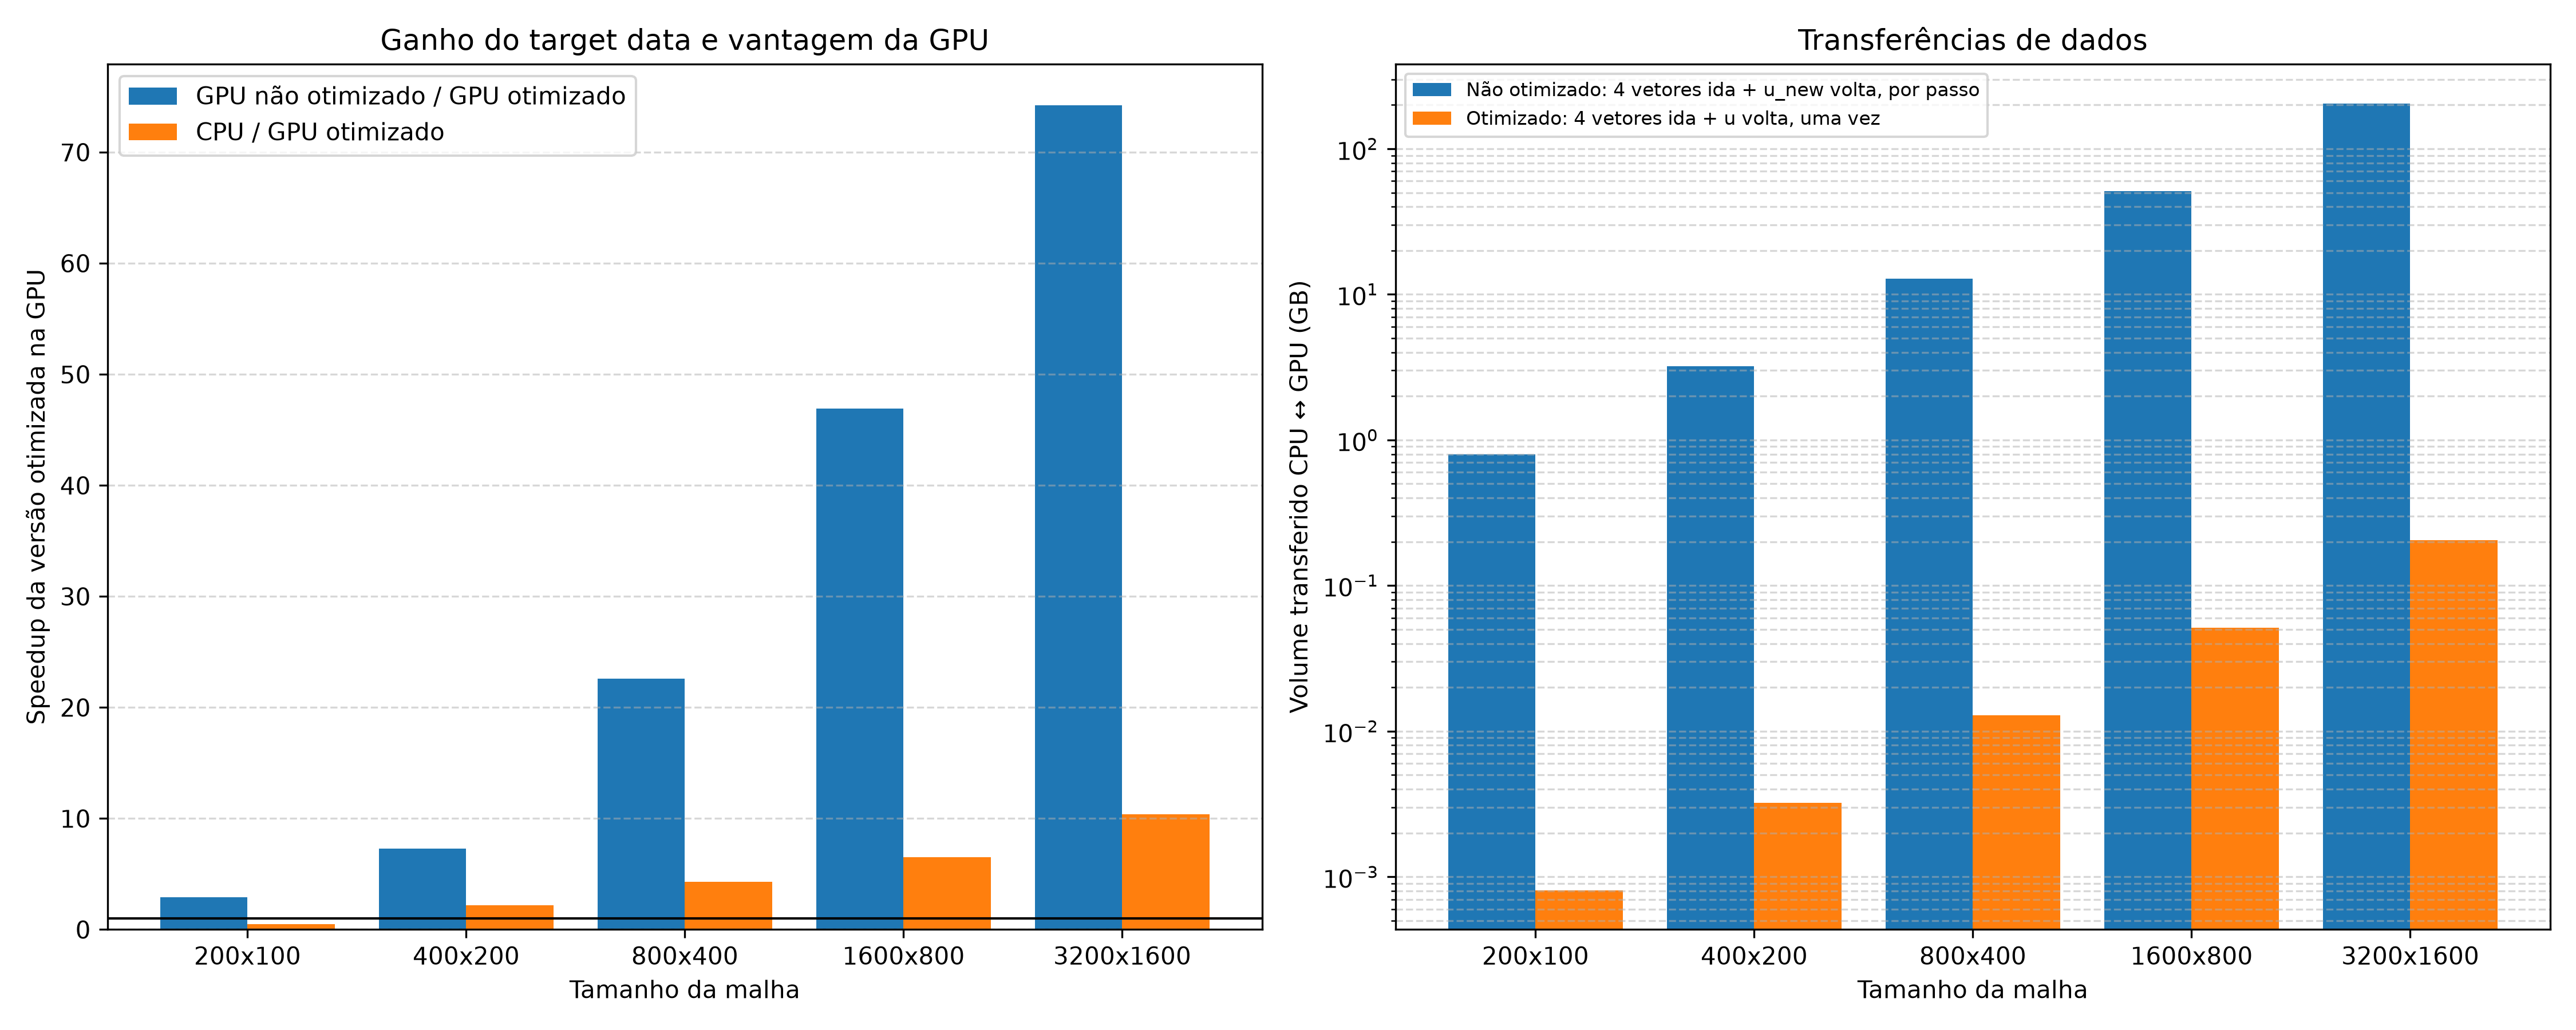
\includegraphics[width=\linewidth]{Tarefa13/tarefa13_otimizacao.png}
			\caption{Tarefa 13 -- À esquerda, \textit{speedup} da versão otimizada na GPU sobre a não otimizada e sobre a execução na CPU; à direita, volume de dados transferido entre CPU e GPU em cada versão.}
		\end{figure}
		\begin{figure}[H]
			\centering
			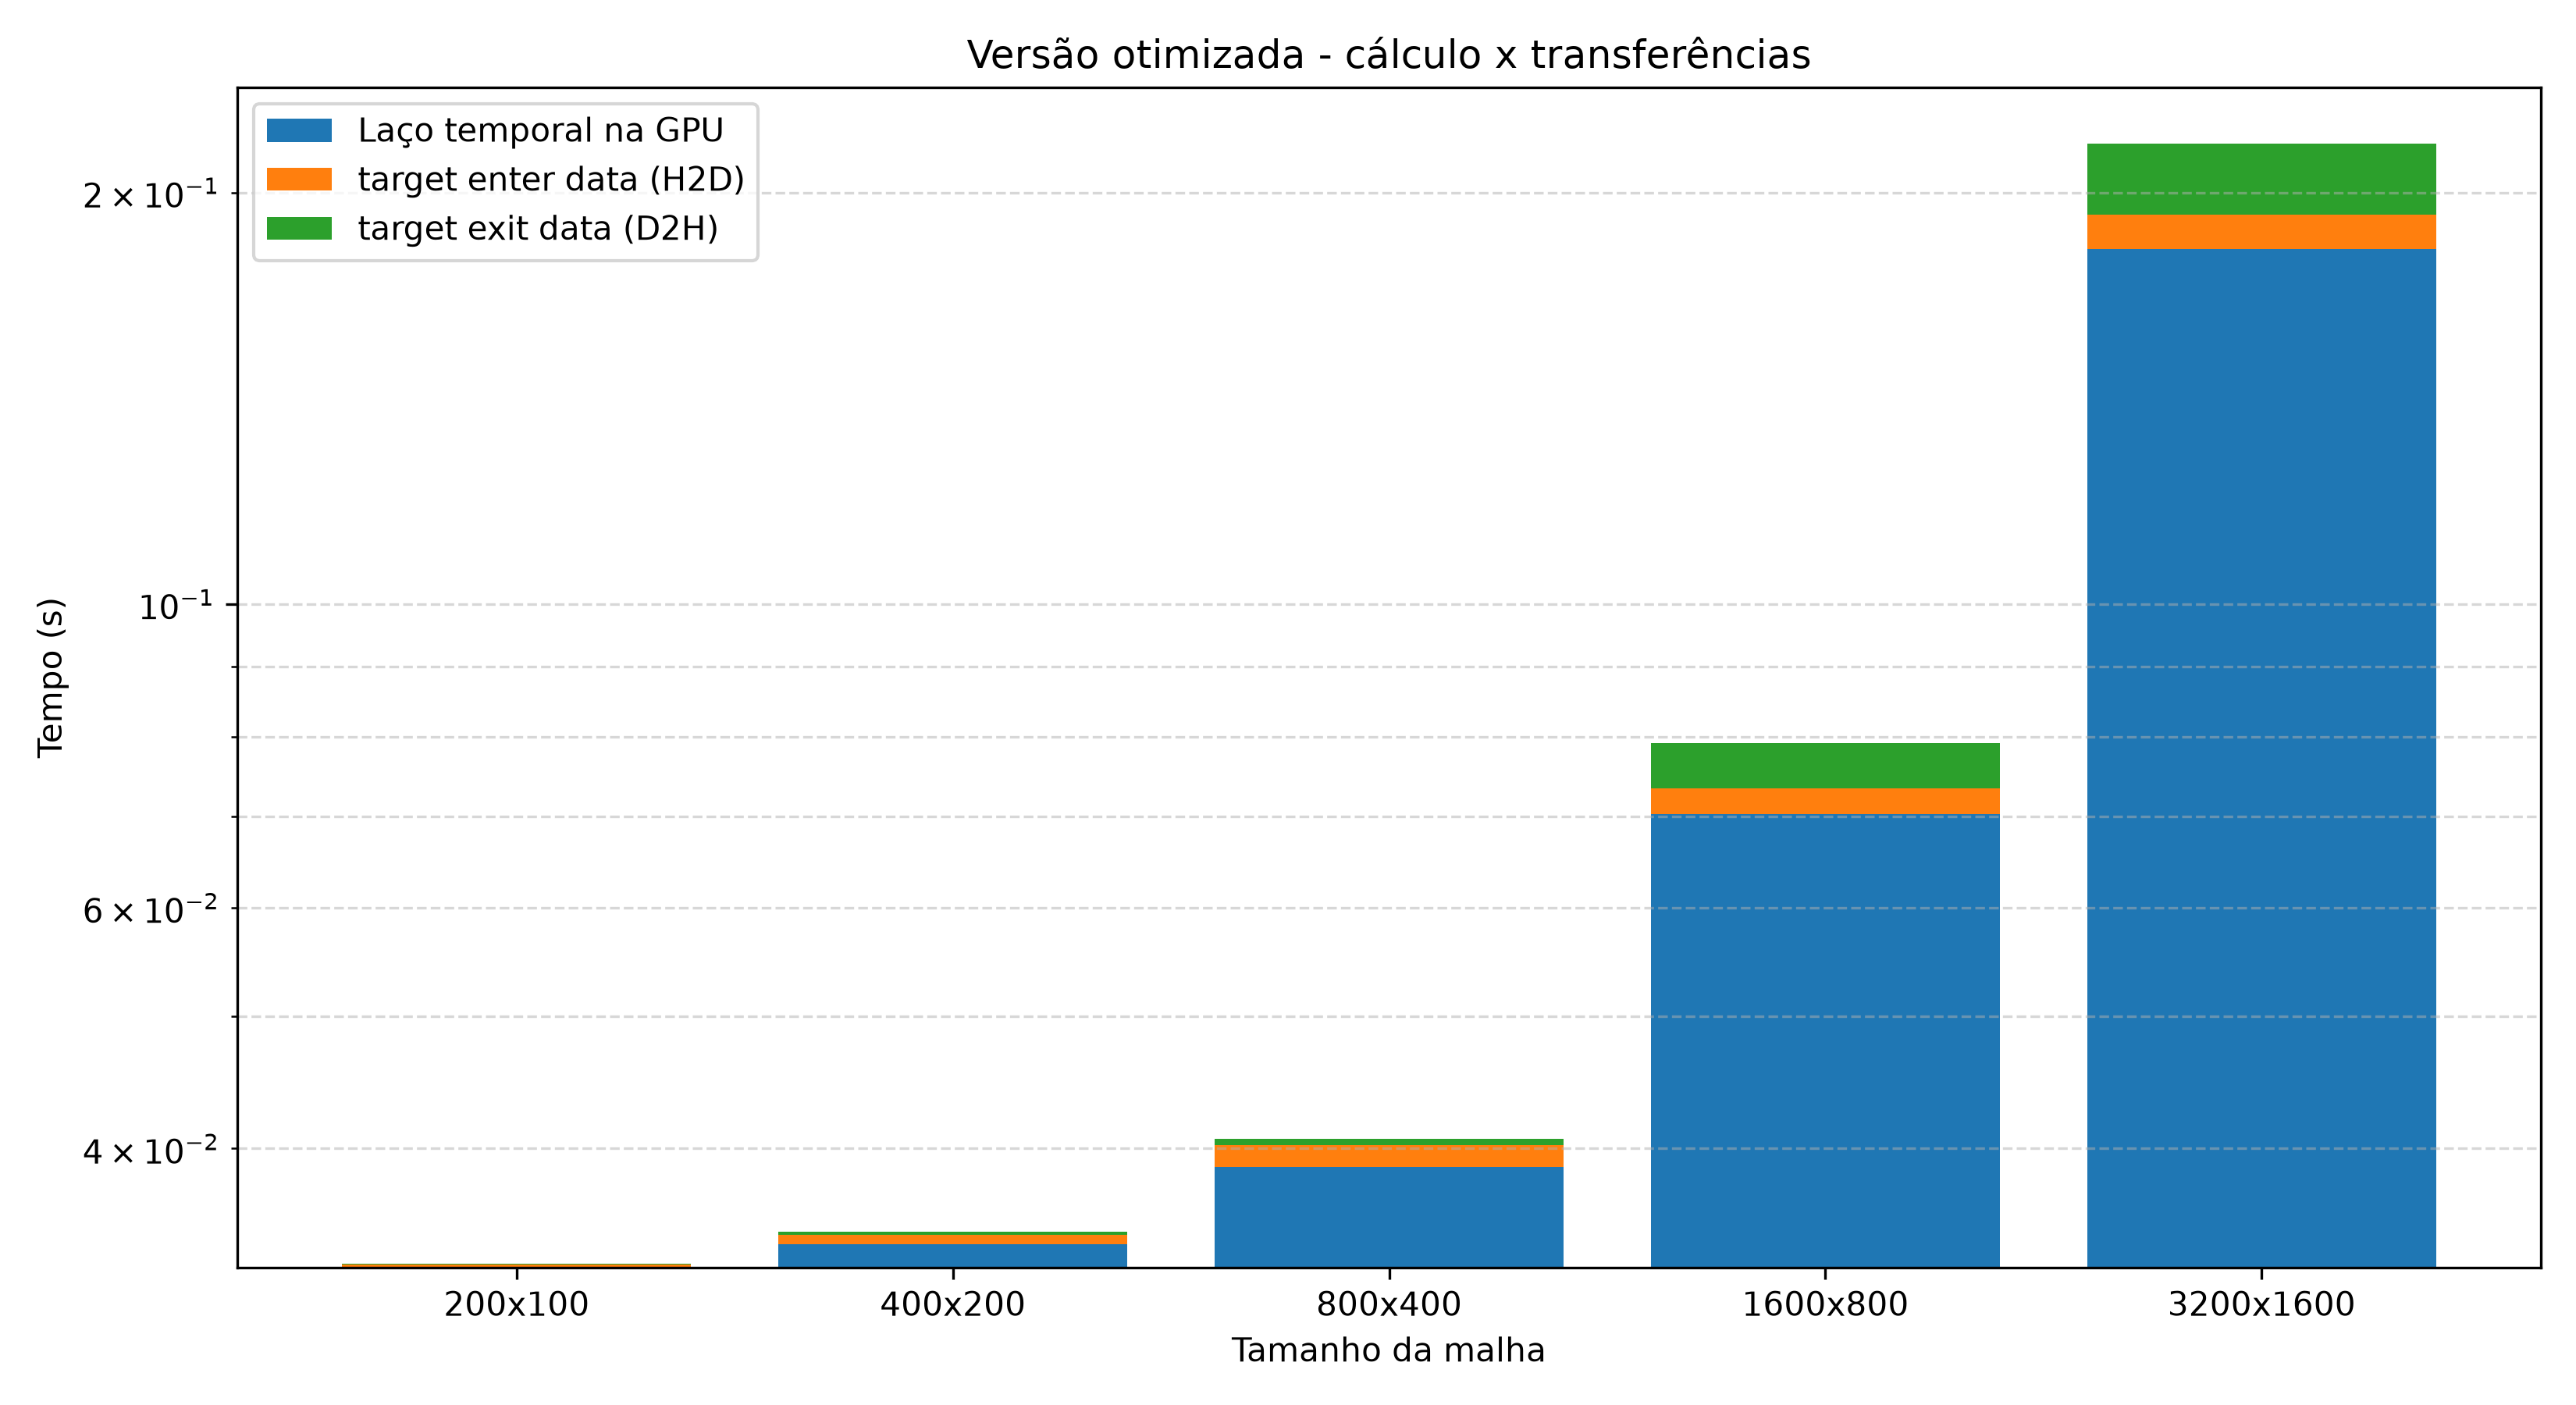
\includegraphics[width=\linewidth]{Tarefa13/tarefa13_transferencias.png}
			\caption{Tarefa 13 -- Versão otimizada: divisão do tempo entre o laço temporal na GPU, a transferência inicial (\texttt{target enter data}) e a final (\texttt{target exit data}).}
		\end{figure}
		\par{
			Analisando os resultados, vemos que a versão não otimizada (azul) possui desempenho um pouco melhor comparado à versão com CPU (verde), porém ainda pior do que todas as alternativas para todos os números estudados.
			
			A versão otimizada demonstra ser muito mais performática do que a não otimizada, pois descarta o maior desafio de performance encontrado nesse problema: a comunicação constante entre o Host e Dispositivo. A versão não otimizada precisa receber, calcular e enviar os dados a cada passo, resultando num crescimento proporcional aos números utilizados. Utilizando otimização com target data, recebimento e envio são feitos apenas uma vez, no início e fim do cálculo, permitindo foco dos recursos na tarefa em si.
			
			A versão otimizada com target data se mostra a melhor para números maiores, porém em malhas pequenas performa pior do que a versão em CPU com paralelização por OpenMP, o que se dá devido ao overhead de inicialização. Como todos os dados são enviados para a GPU logo de início (um custo que varia de acordo com a taxa de transferência do meio e tamanho dos dados a serem enviados), para malhas pequenas como 200x100, esse custo é quase o mesmo tempo do cálculo na GPU, o que torna esse método inefetivo em otimizar o problema.
			
			Portanto, podemos optar por usar um modo híbrido, que utiliza a paralelização em CPU para números pequenos, optando pela versão otimizada em GPU a partir do ponto em que o overhead passa a ser descartável.
		}
		\subsection{\subtTres}
		\begin{lstlisting}[language=c]
		\end{lstlisting}
		
	\newpage
		\onehalfspacing
		\section{TAREFA 14}
		\subsection{\subtUm}
		\par{Texto}
		\subsection{\subtDois}
		
		\begin{figure}[H]
			\centering
			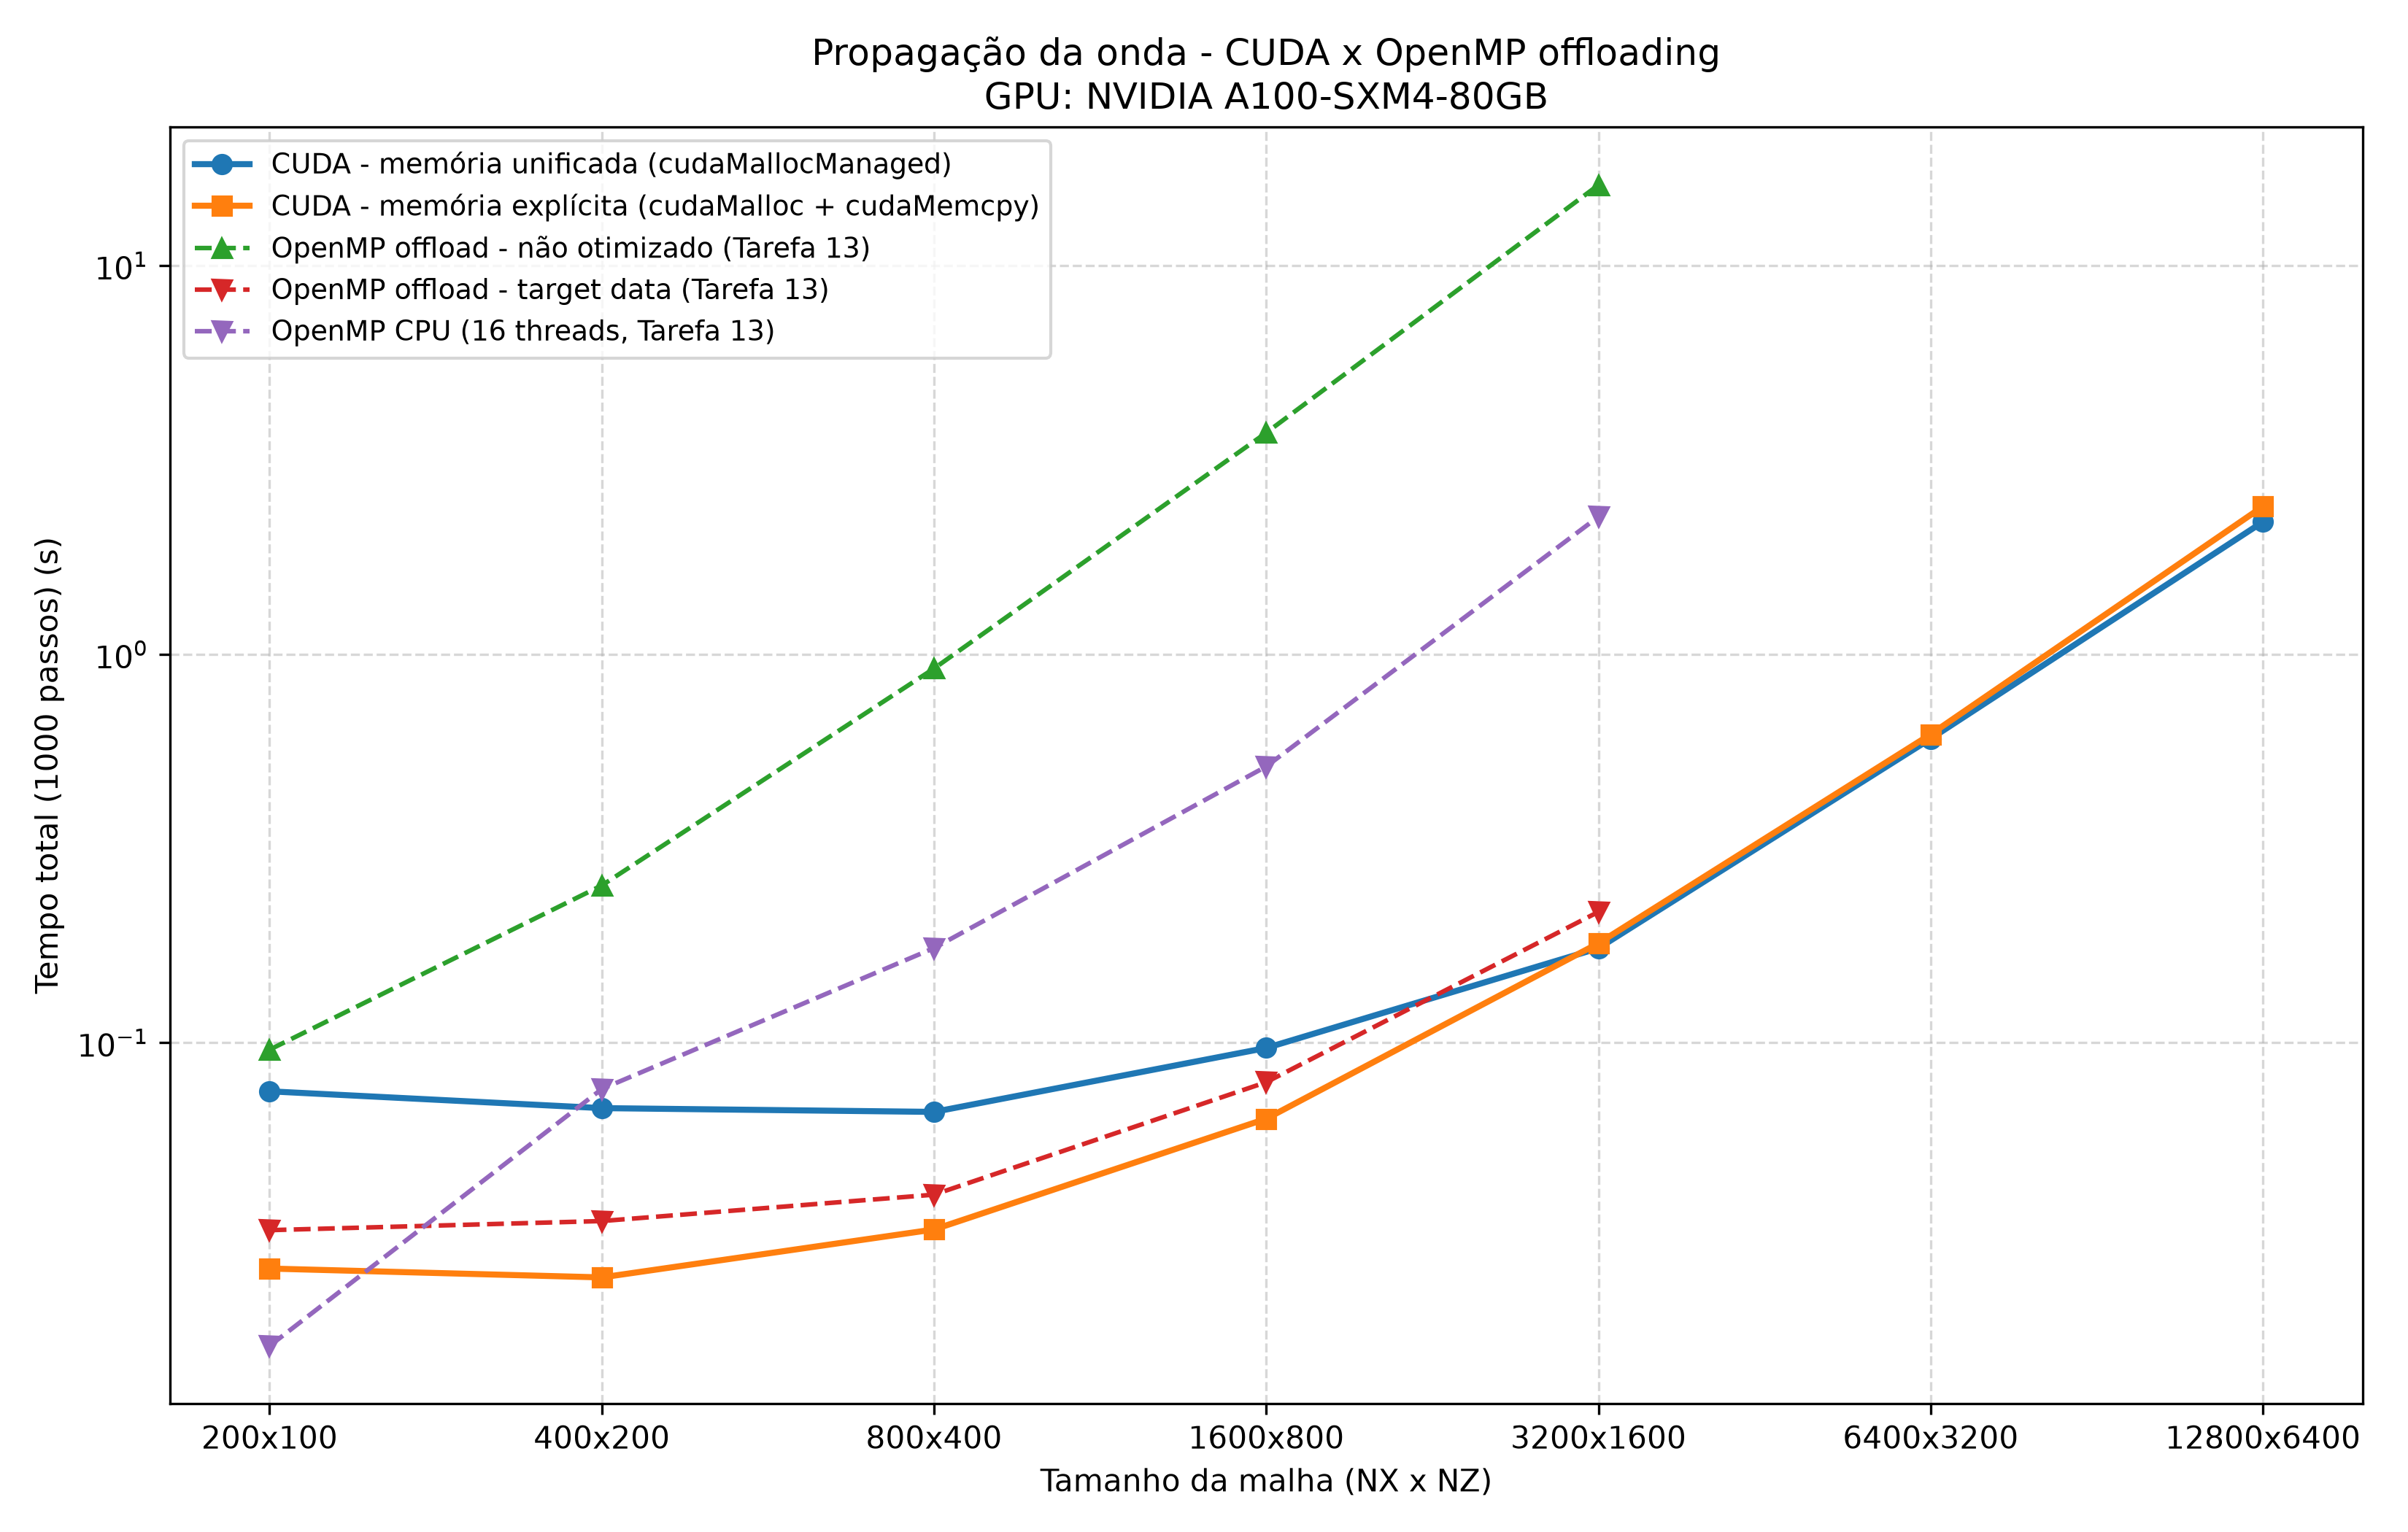
\includegraphics[width=\linewidth]{Tarefa14/tarefa14_tempos.png}
		\end{figure}
		\begin{figure}[H]
			\centering
			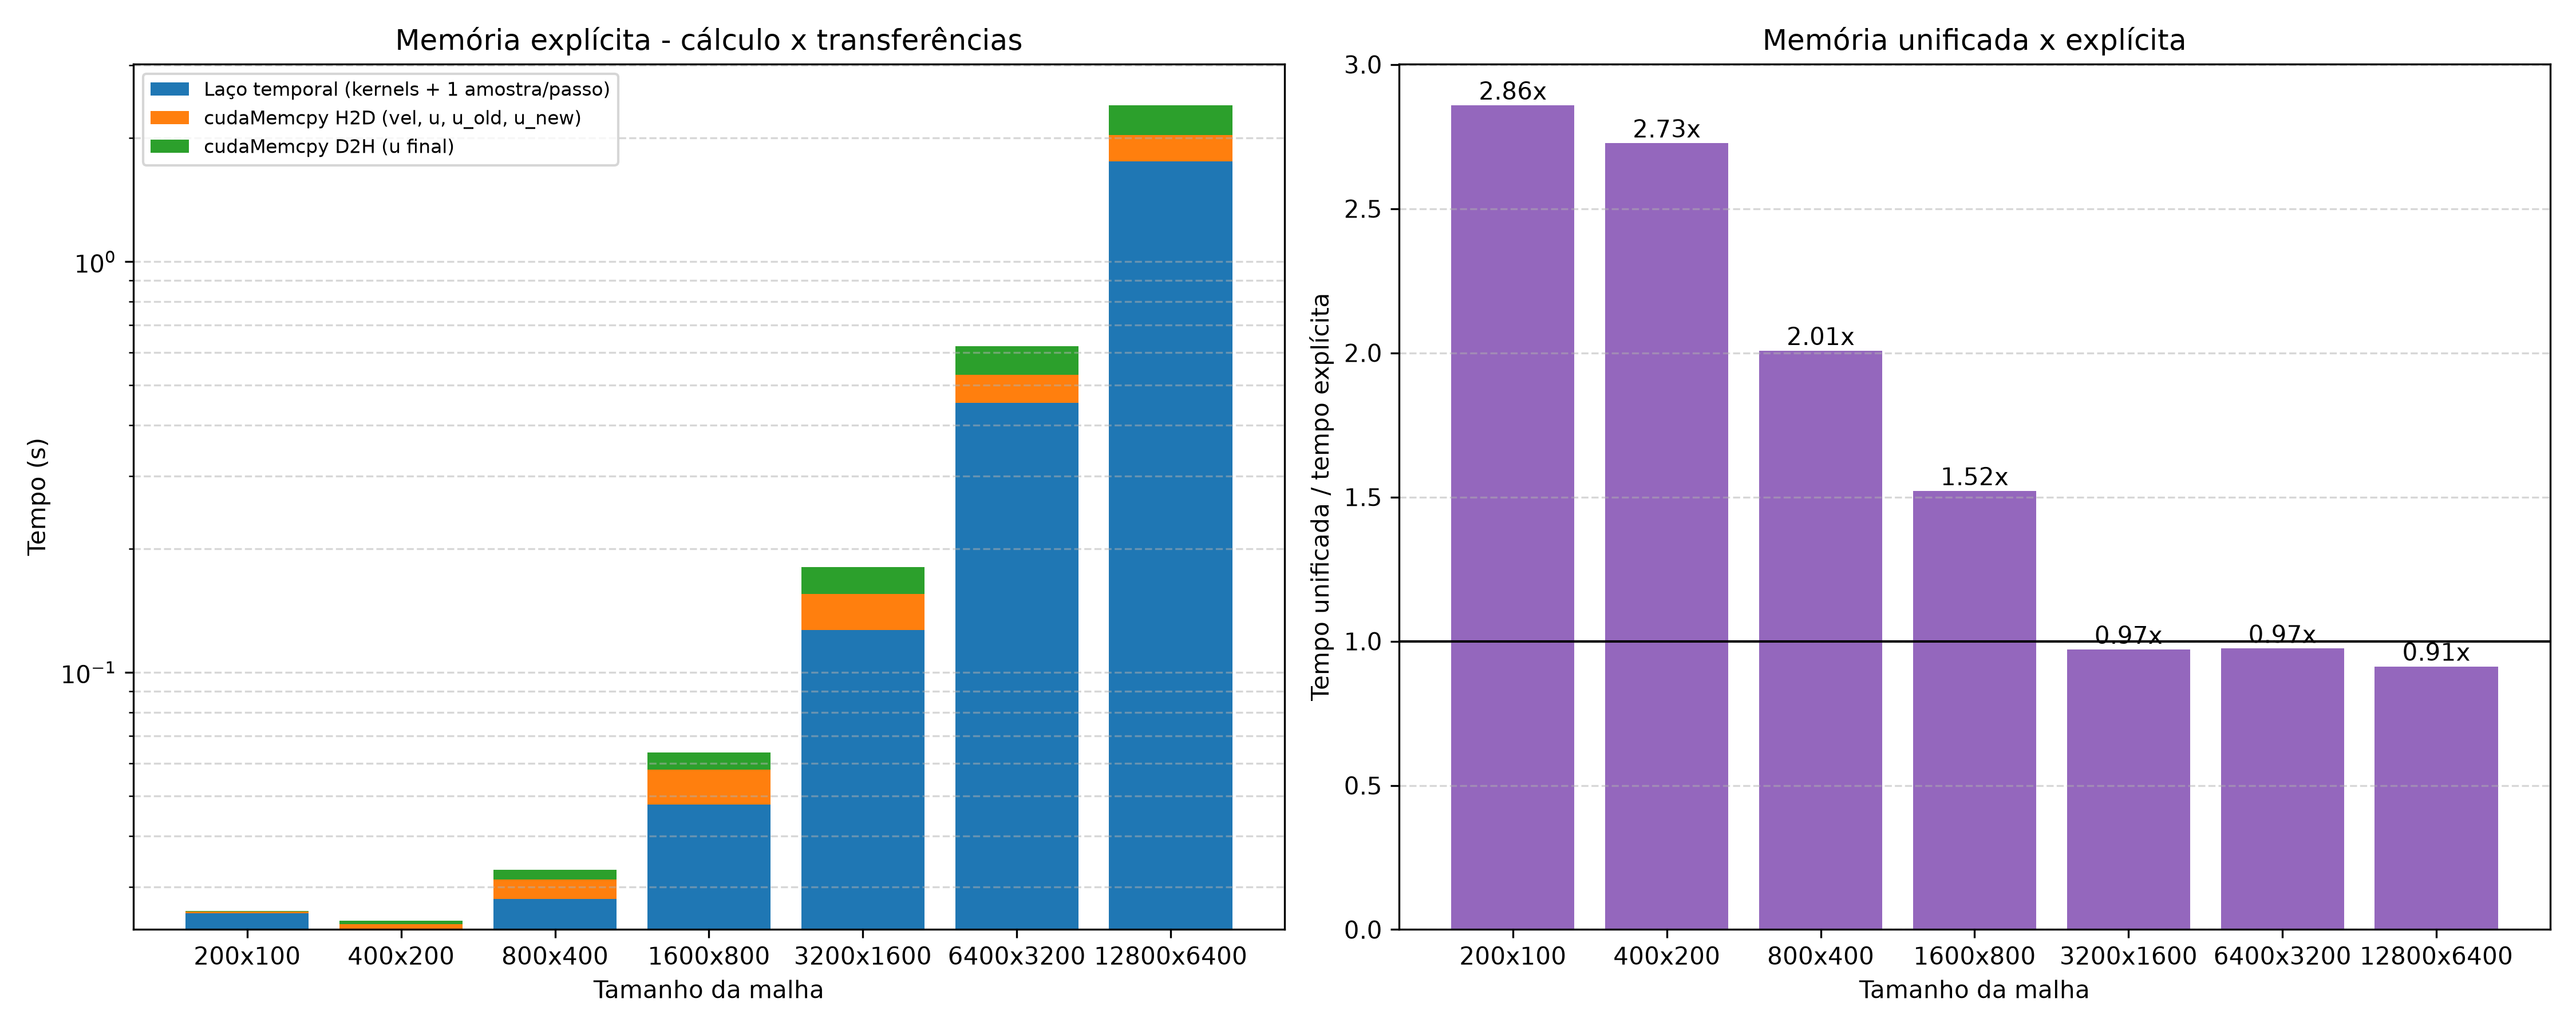
\includegraphics[width=\linewidth]{Tarefa14/tarefa14_memoria.png}
		\end{figure}
		\par{
			Analisando o gráfico de comparações entre os códigos em CUDA com memória unificada, explicita, offload em OPENMP com e sem otimização e paralelização em CPU, feito a partir do supercomputador NPAD, podemos verificar que ambas as versões com cuda se mostram mais performáticas do que todas as alternativas a partir de malhas 3200x1600.
			
			É possível notar, também, que a opção por memória unificada, apesar de iniciar mais lenta do que a opção por memória explicita, ao longo do tempo diminui a diferença entre eles, chegando a ultrapassar em performance a partir de malhas 12800x6400. Isso se dá pois a versão explícita copia mais dados do que a unificada, aumentando de acordo com o tamanho da malha, enquanto o custo extra da unificada é fixo
			
			Portanto, identificamos que as versões em CUDA são mais vantajosas quando lidando com problemas de grande escala, sendo ideal para tarefas de inteligência artificial, por exemplo.
		}
		\subsection{\subtTres}
		\begin{lstlisting}[language=c]
		\end{lstlisting}
			
	\newpage
		\onehalfspacing
		\section{TAREFA 15}
		\subsection{\subtUm}
		\par{Texto}
		\subsection{\subtDois}
		\par{Texto}
		\begin{figure}[H]
			\centering
			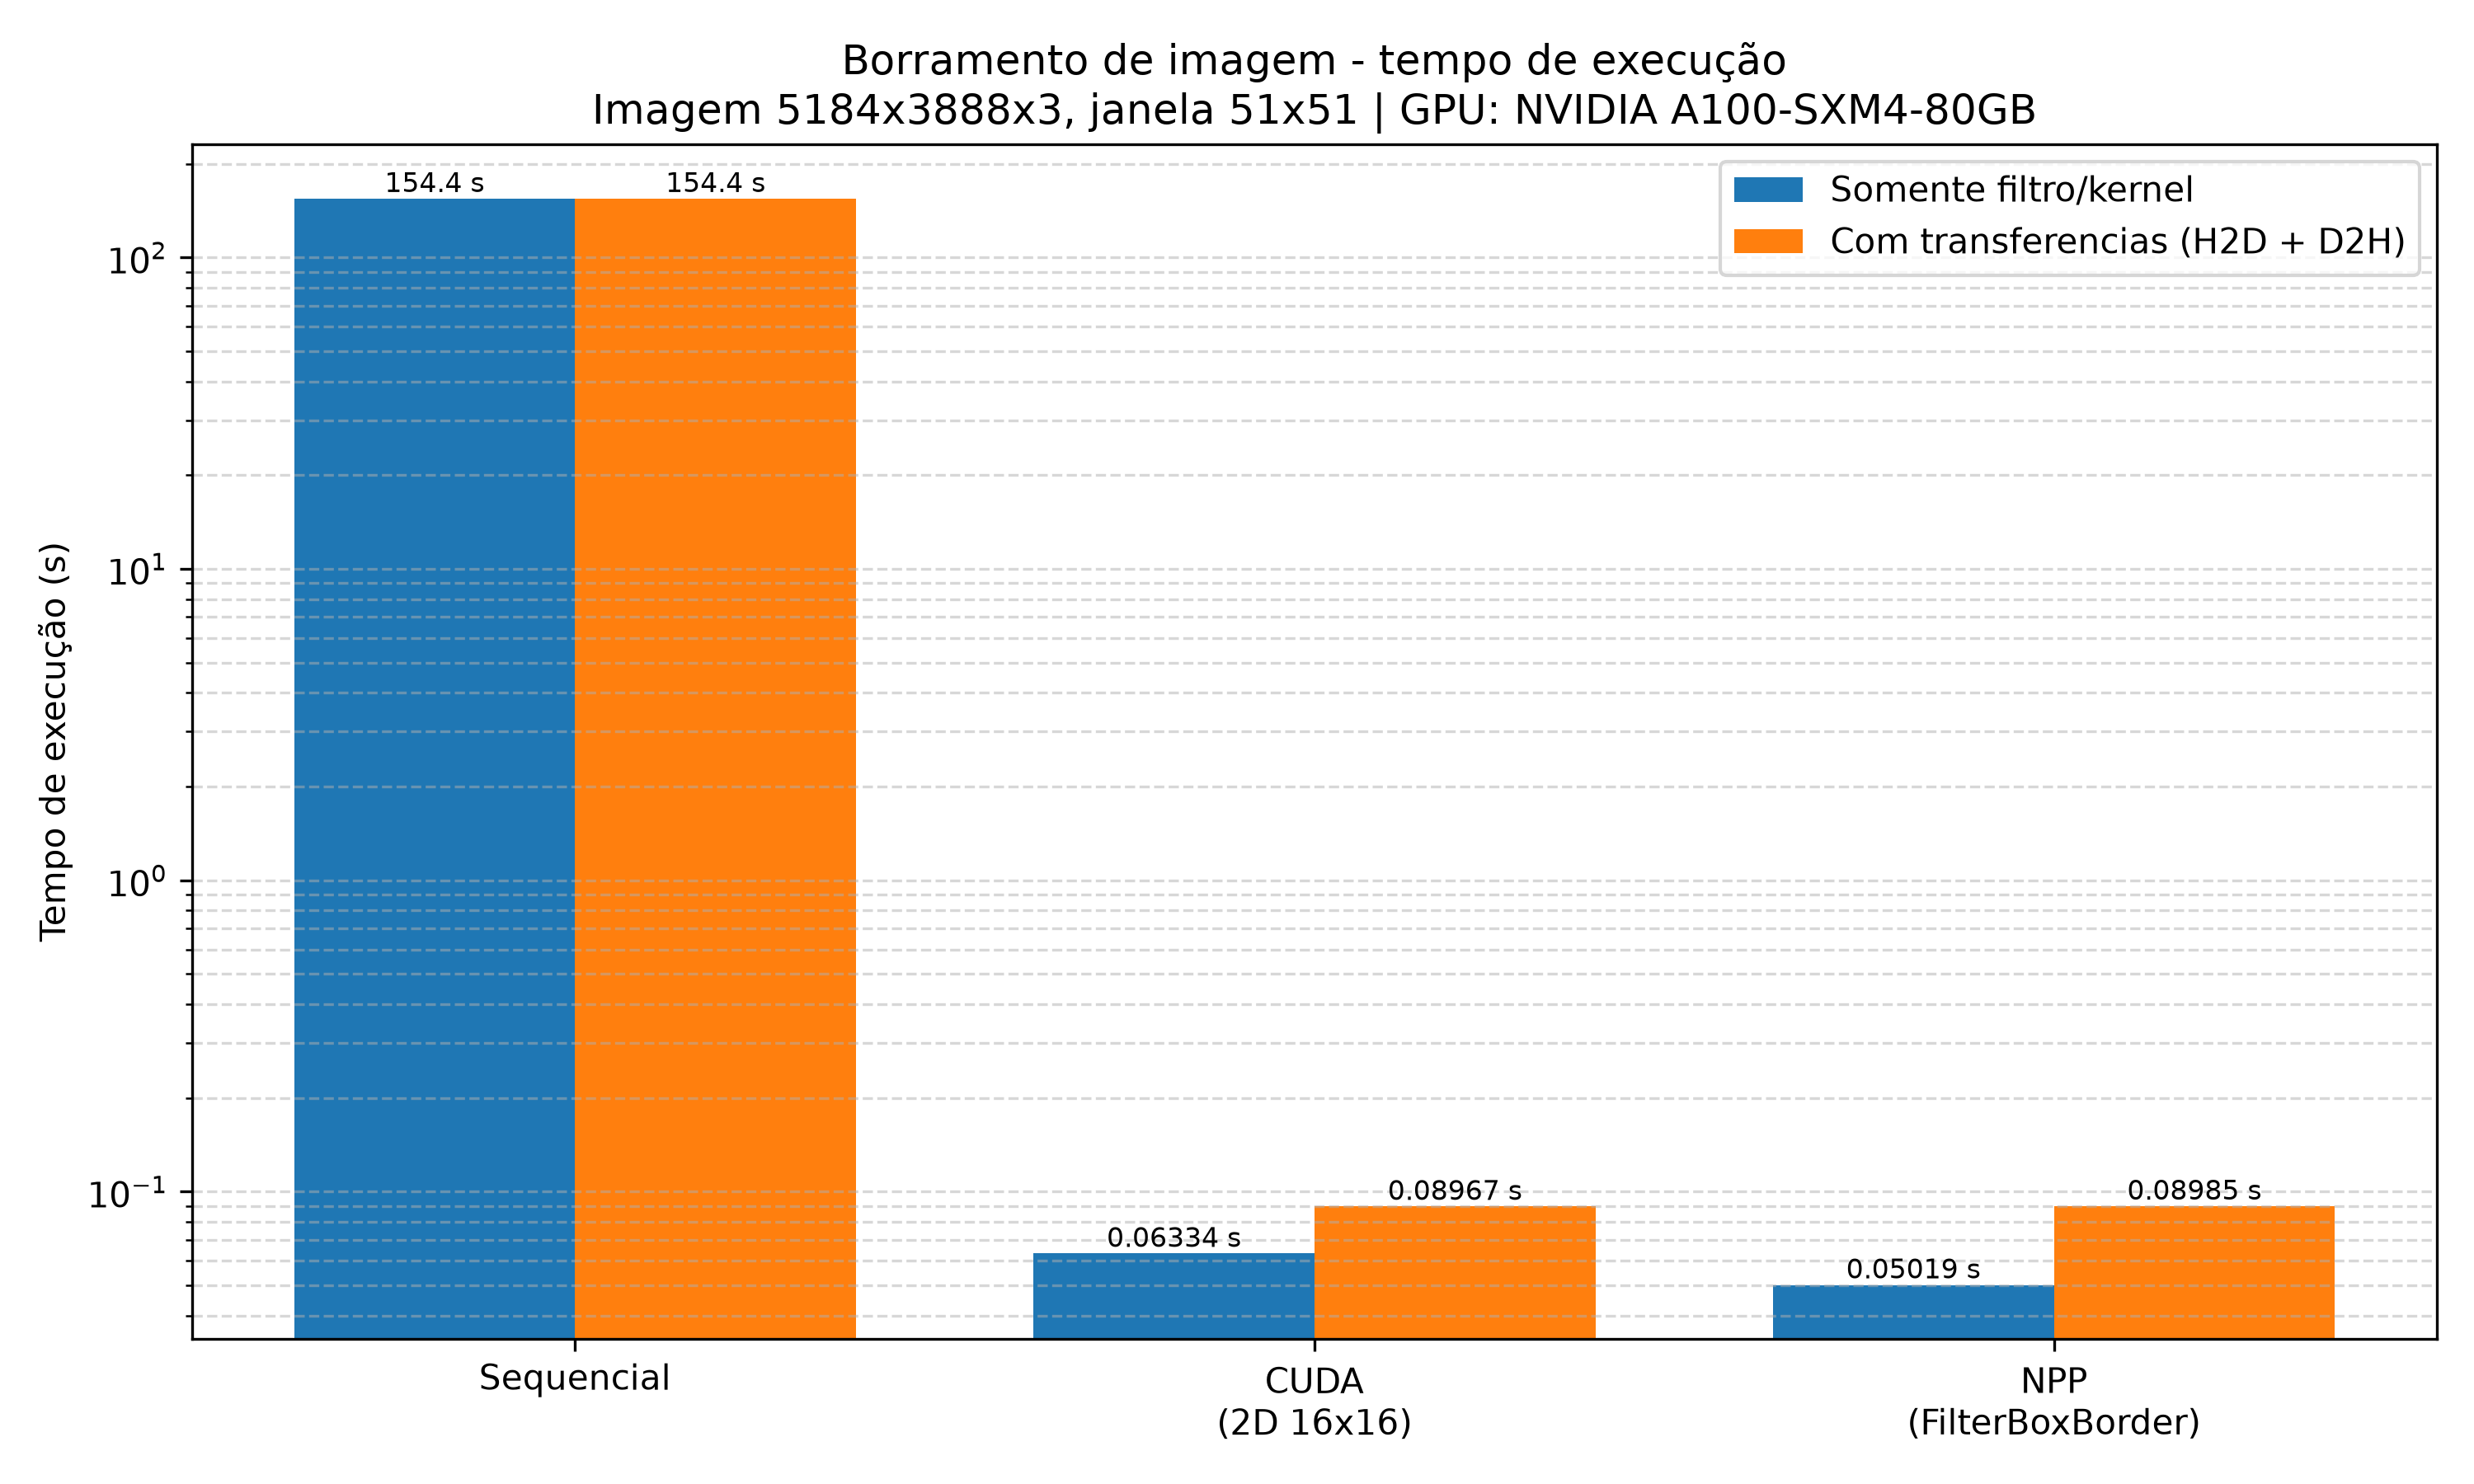
\includegraphics[width=\linewidth]{Tarefa15/tarefa15_tempos.png}
		\end{figure}
		\begin{figure}[H]
			\centering
			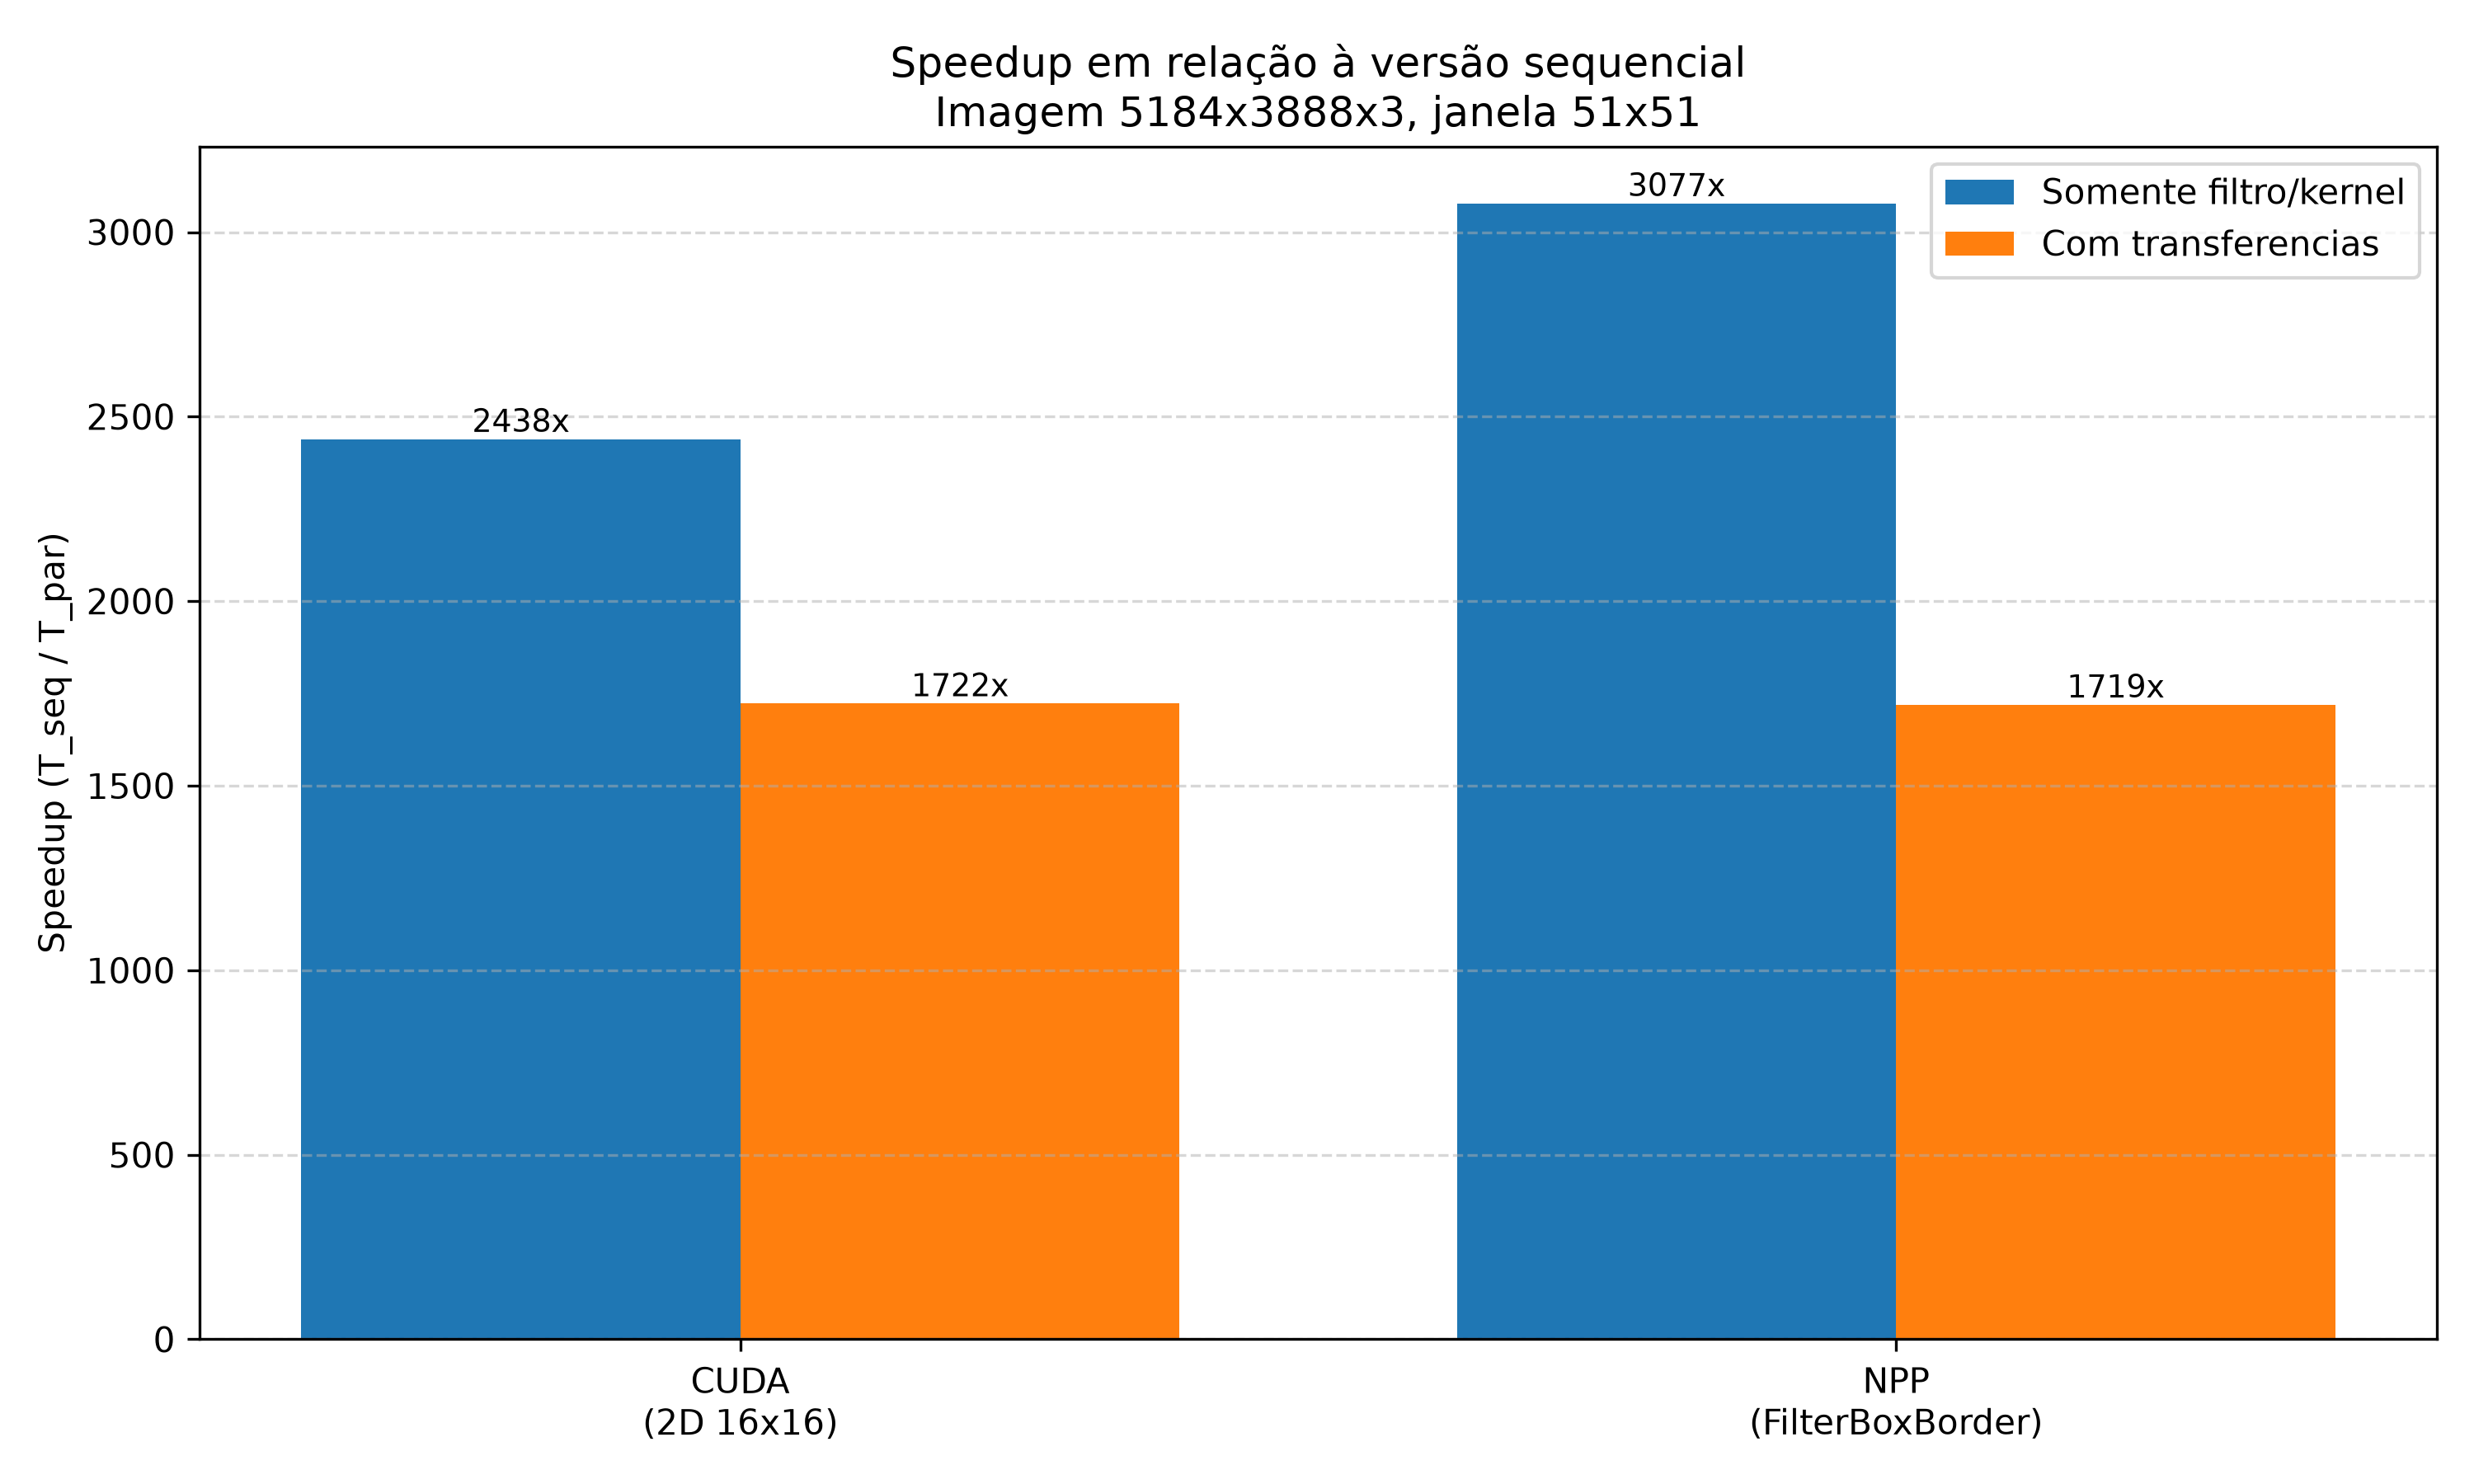
\includegraphics[width=\linewidth]{Tarefa15/tarefa15_speedup.png}
		\end{figure}
		\begin{figure}[H]
			\centering
			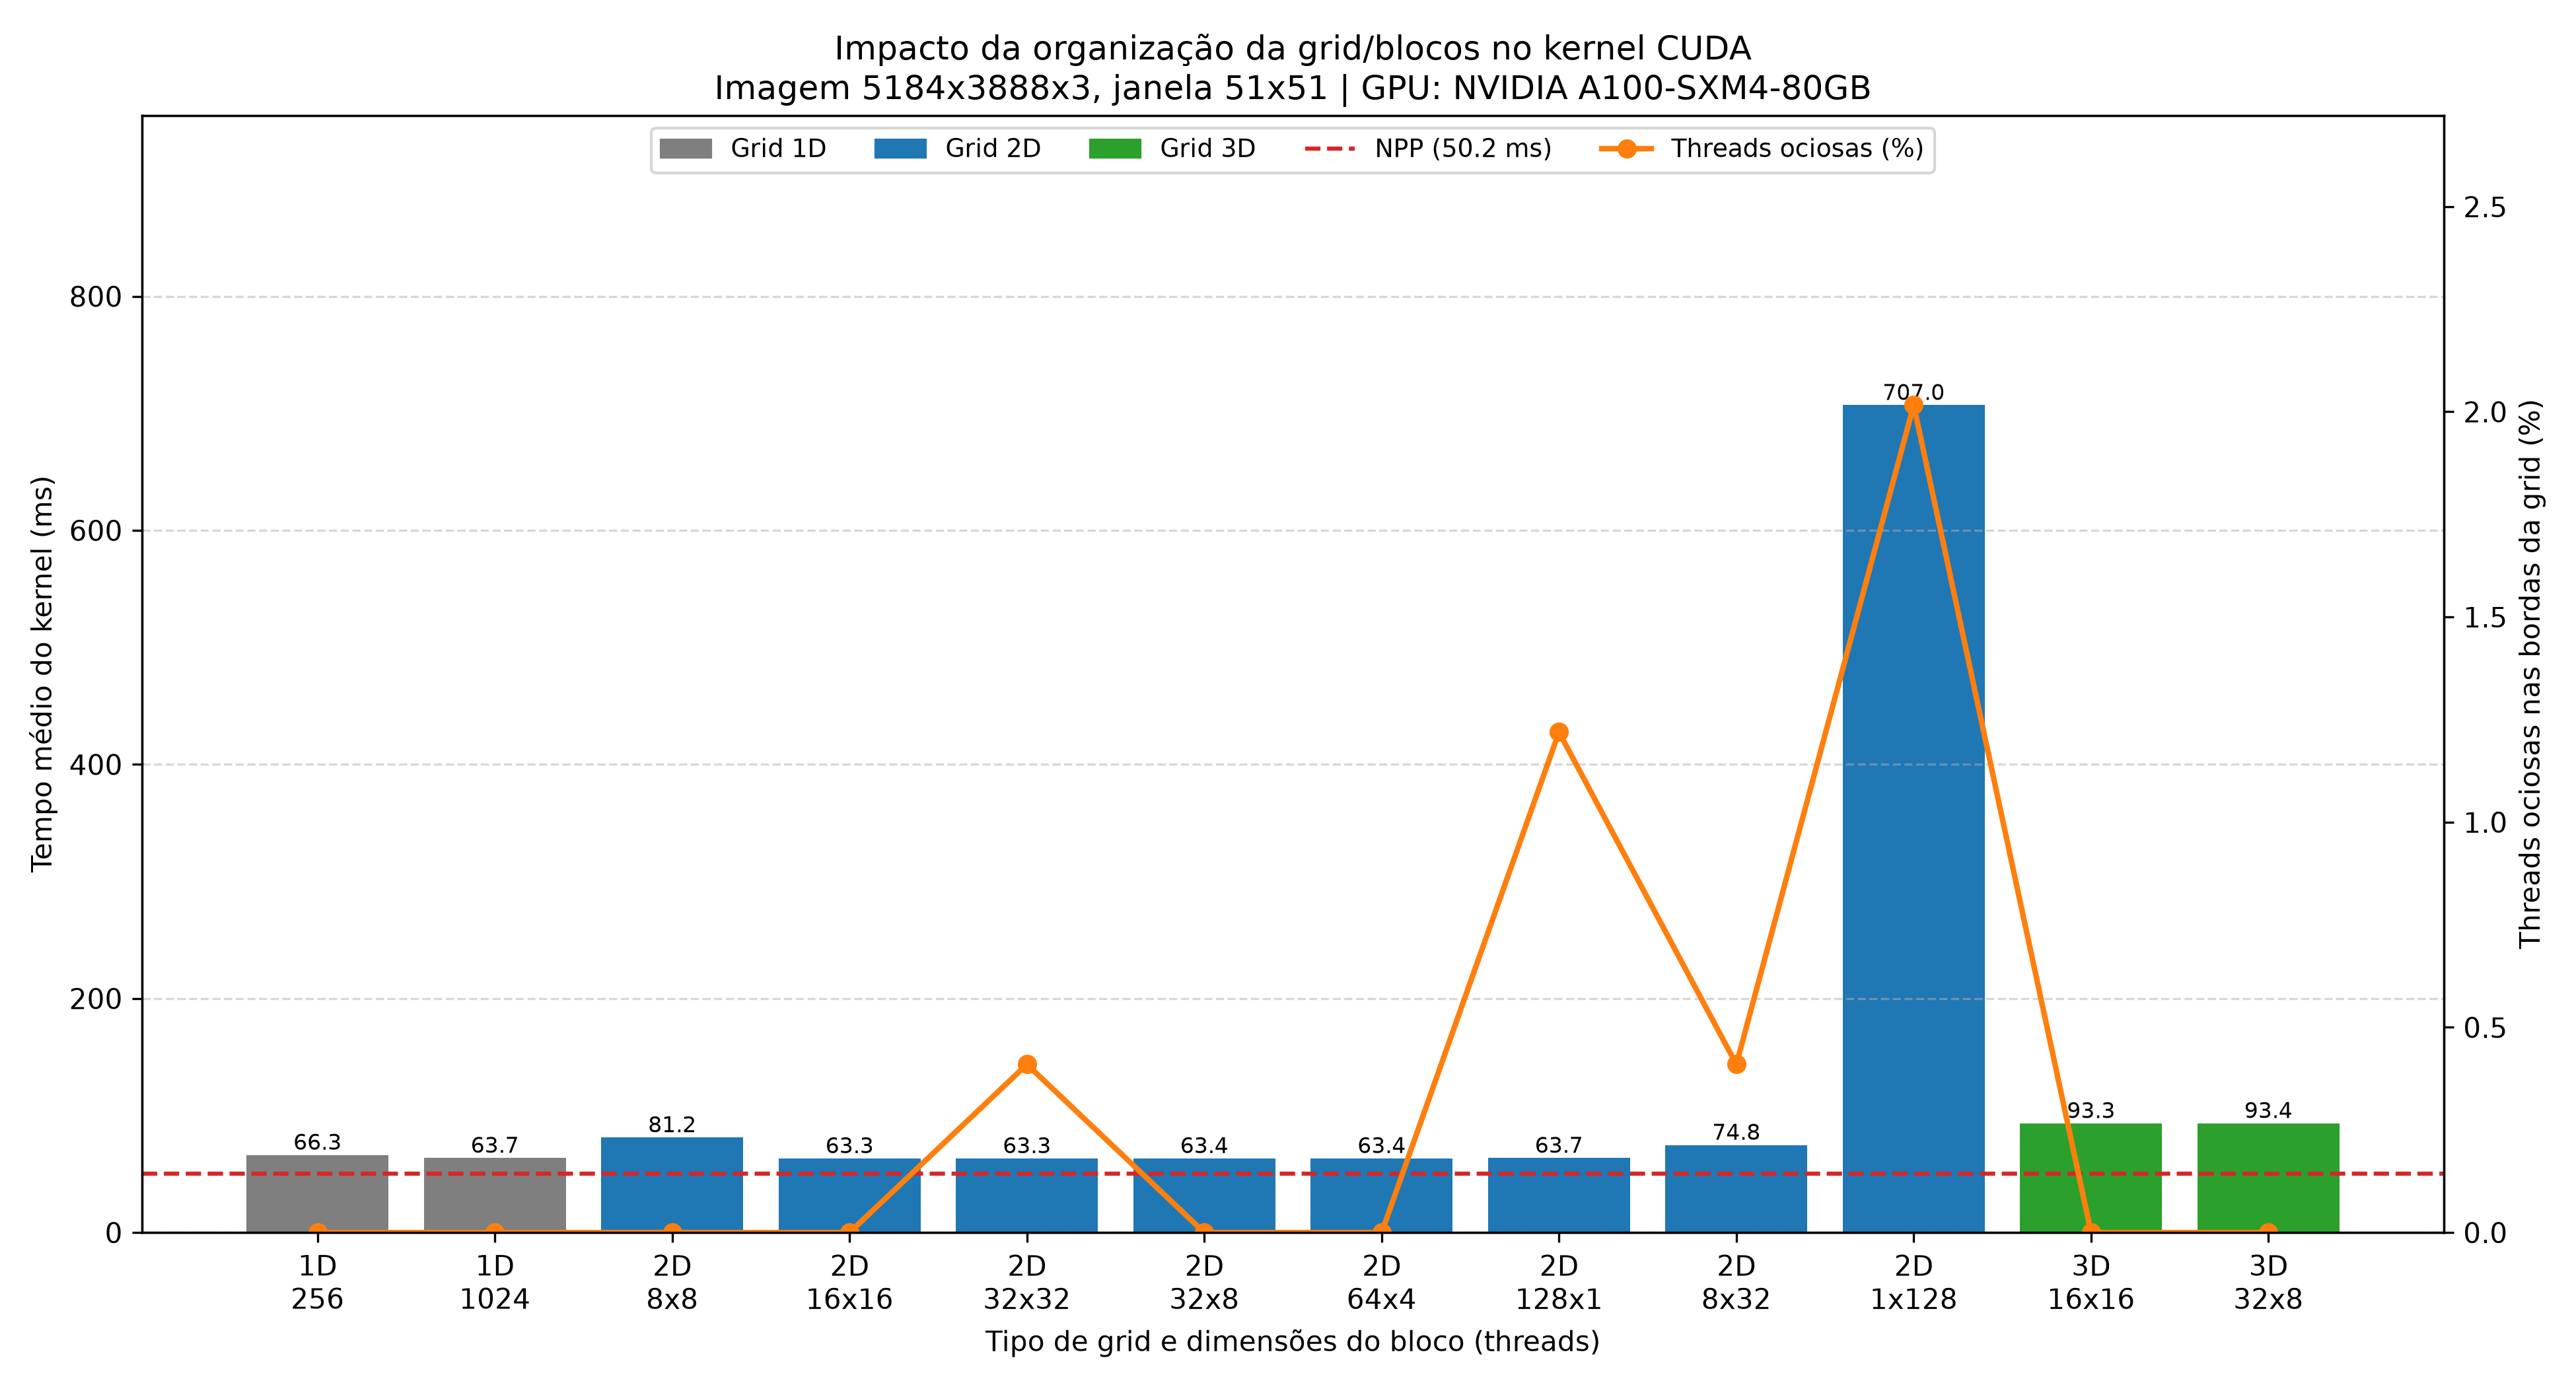
\includegraphics[width=\linewidth]{Tarefa15/tarefa15_grid.png}
			\caption{Tarefa 15 -- Tempo médio do kernel para cada organização de grid (1D, 2D e 3D) e dimensão de bloco, com o percentual de threads ociosas nas bordas da grid; a linha tracejada indica o tempo do filtro do NPP.}
		\end{figure}
		\subsection{\subtTres}
		\begin{lstlisting}[language=c]
		\end{lstlisting}
		
	\newpage
		\onehalfspacing
		\section{TAREFA 16}
		\subsection{\subtUm}
		\par{Texto}
		\subsection{\subtDois}
		\par{Texto}
		\begin{figure}[H]
			\centering
			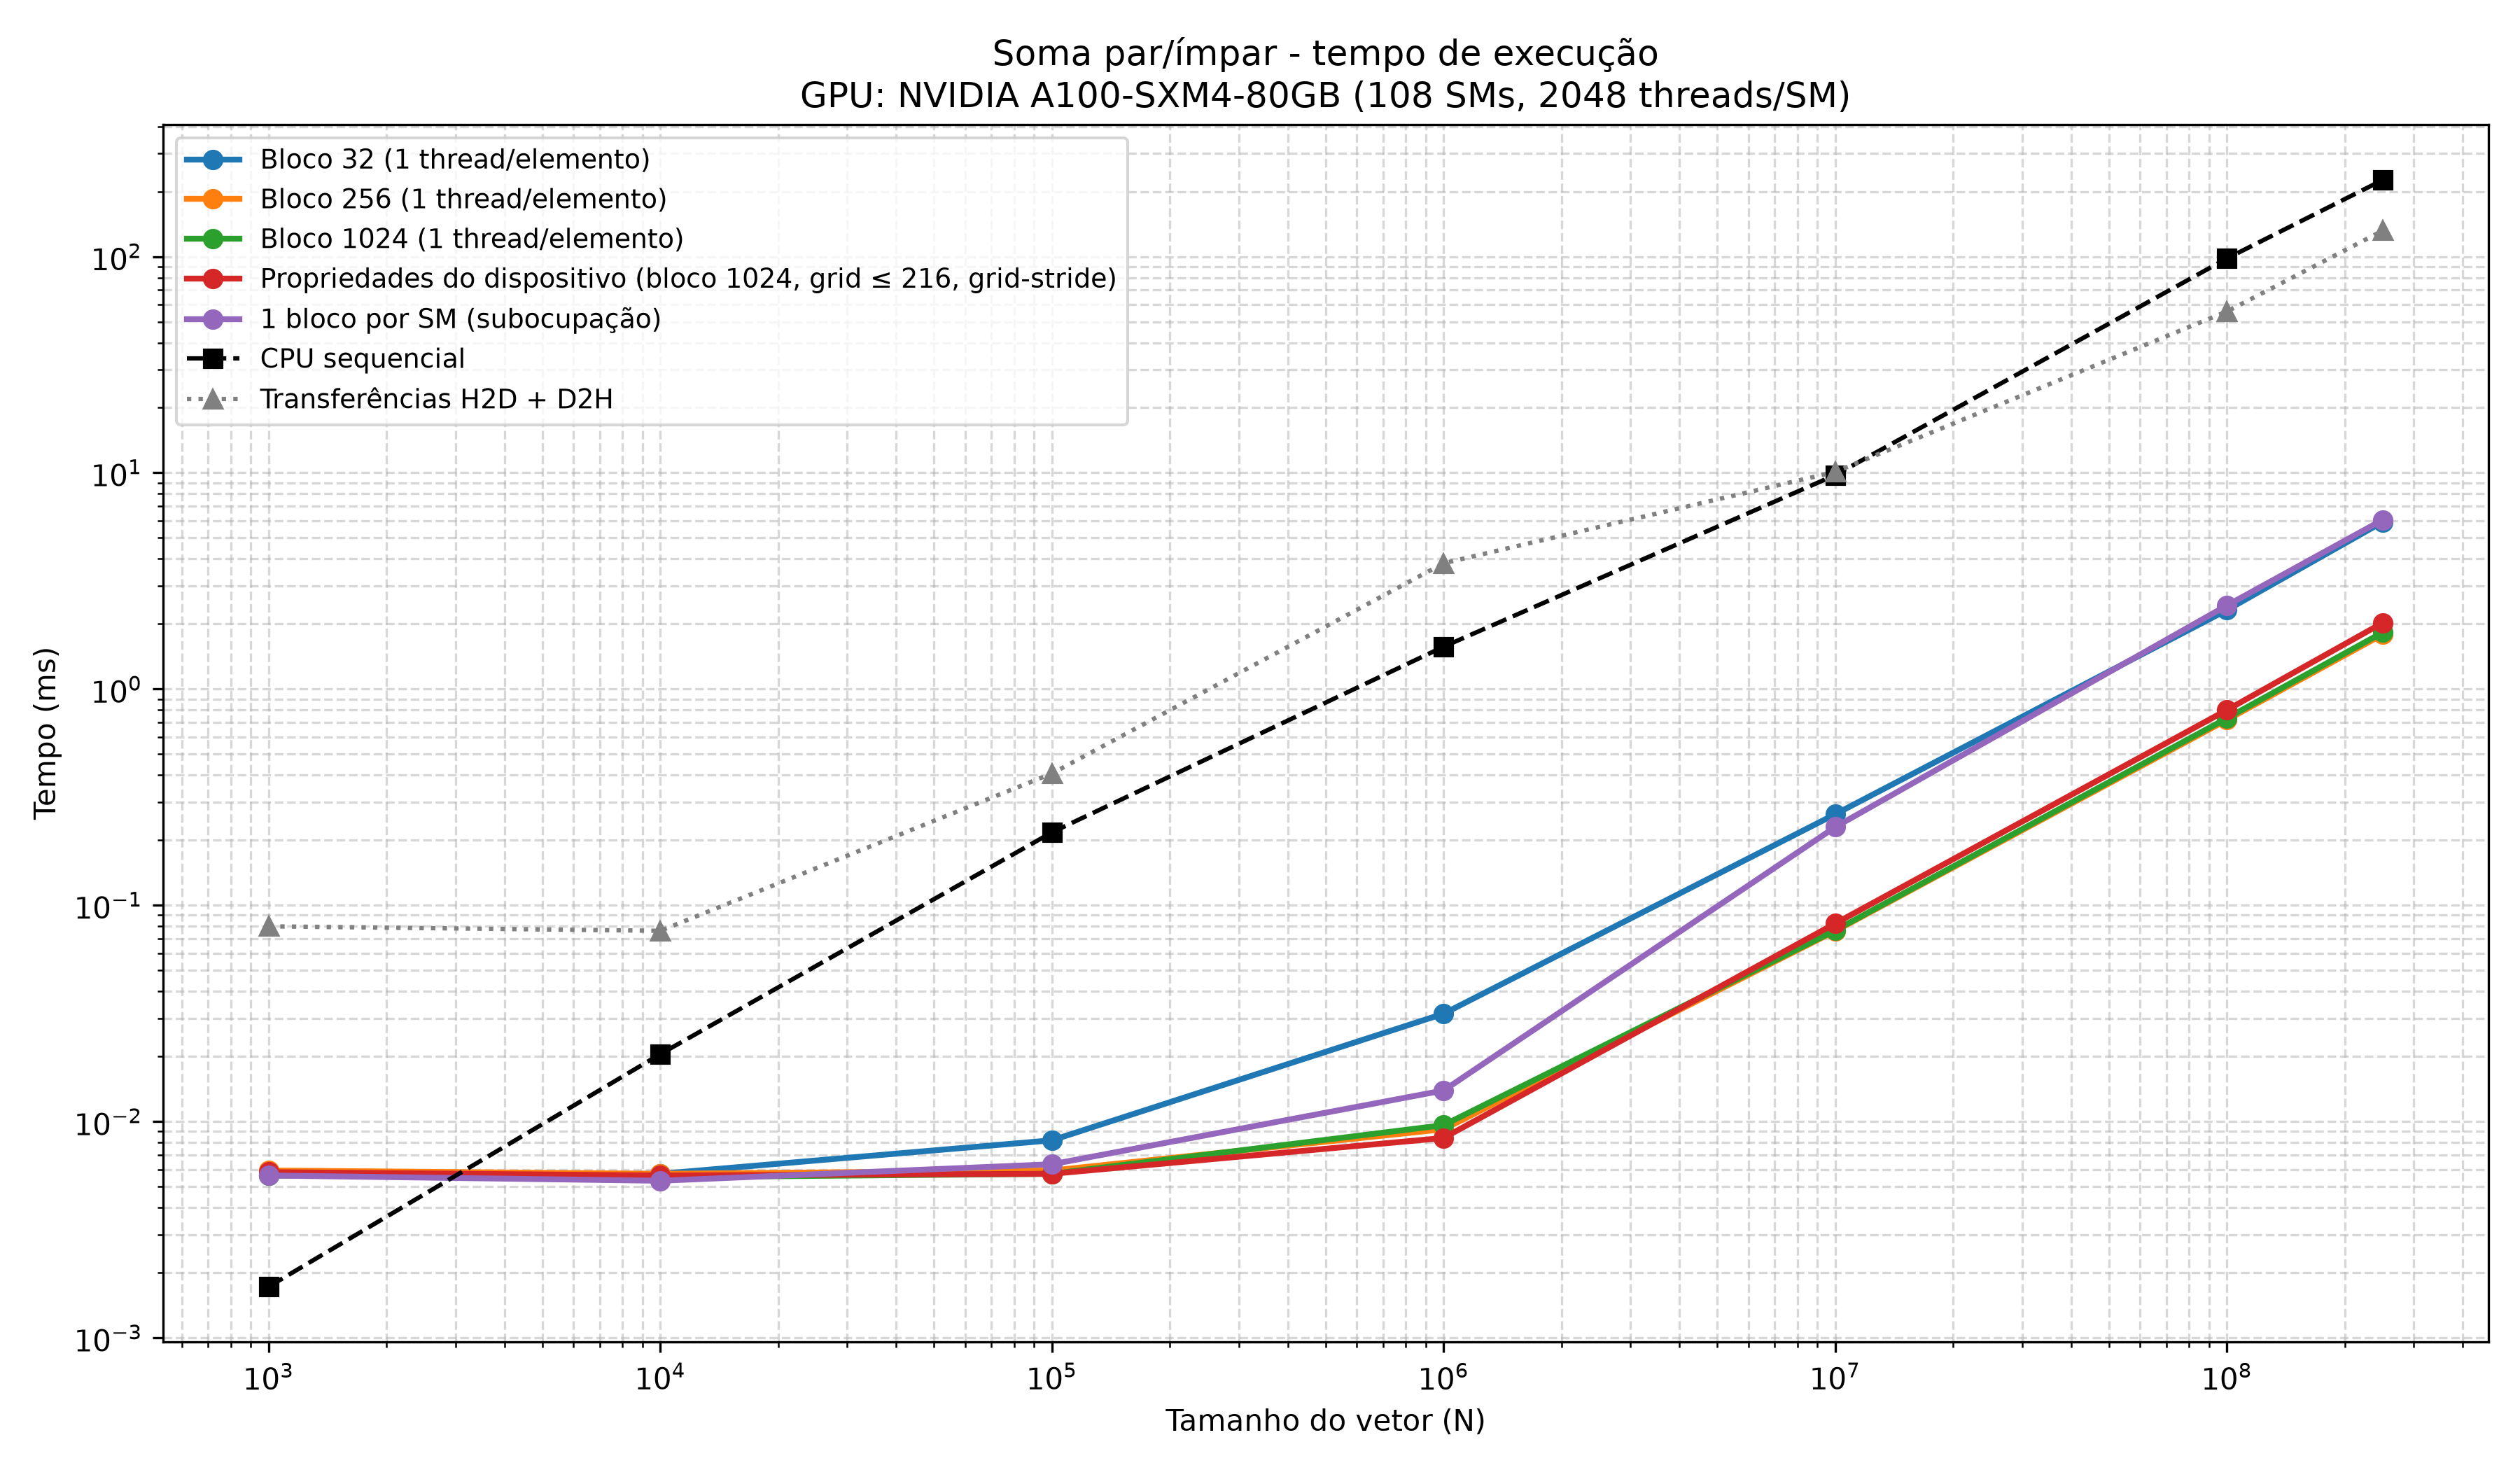
\includegraphics[width=\linewidth]{Tarefa16/tarefa16_tempos.png}
			\caption{Tarefa 16 -- Tempo do kernel de soma par/ímpar em função do tamanho do vetor para diferentes configurações de grid e bloco, comparado à CPU sequencial e ao custo das transferências H2D e D2H.}
		\end{figure}
		\begin{figure}[H]
			\centering
			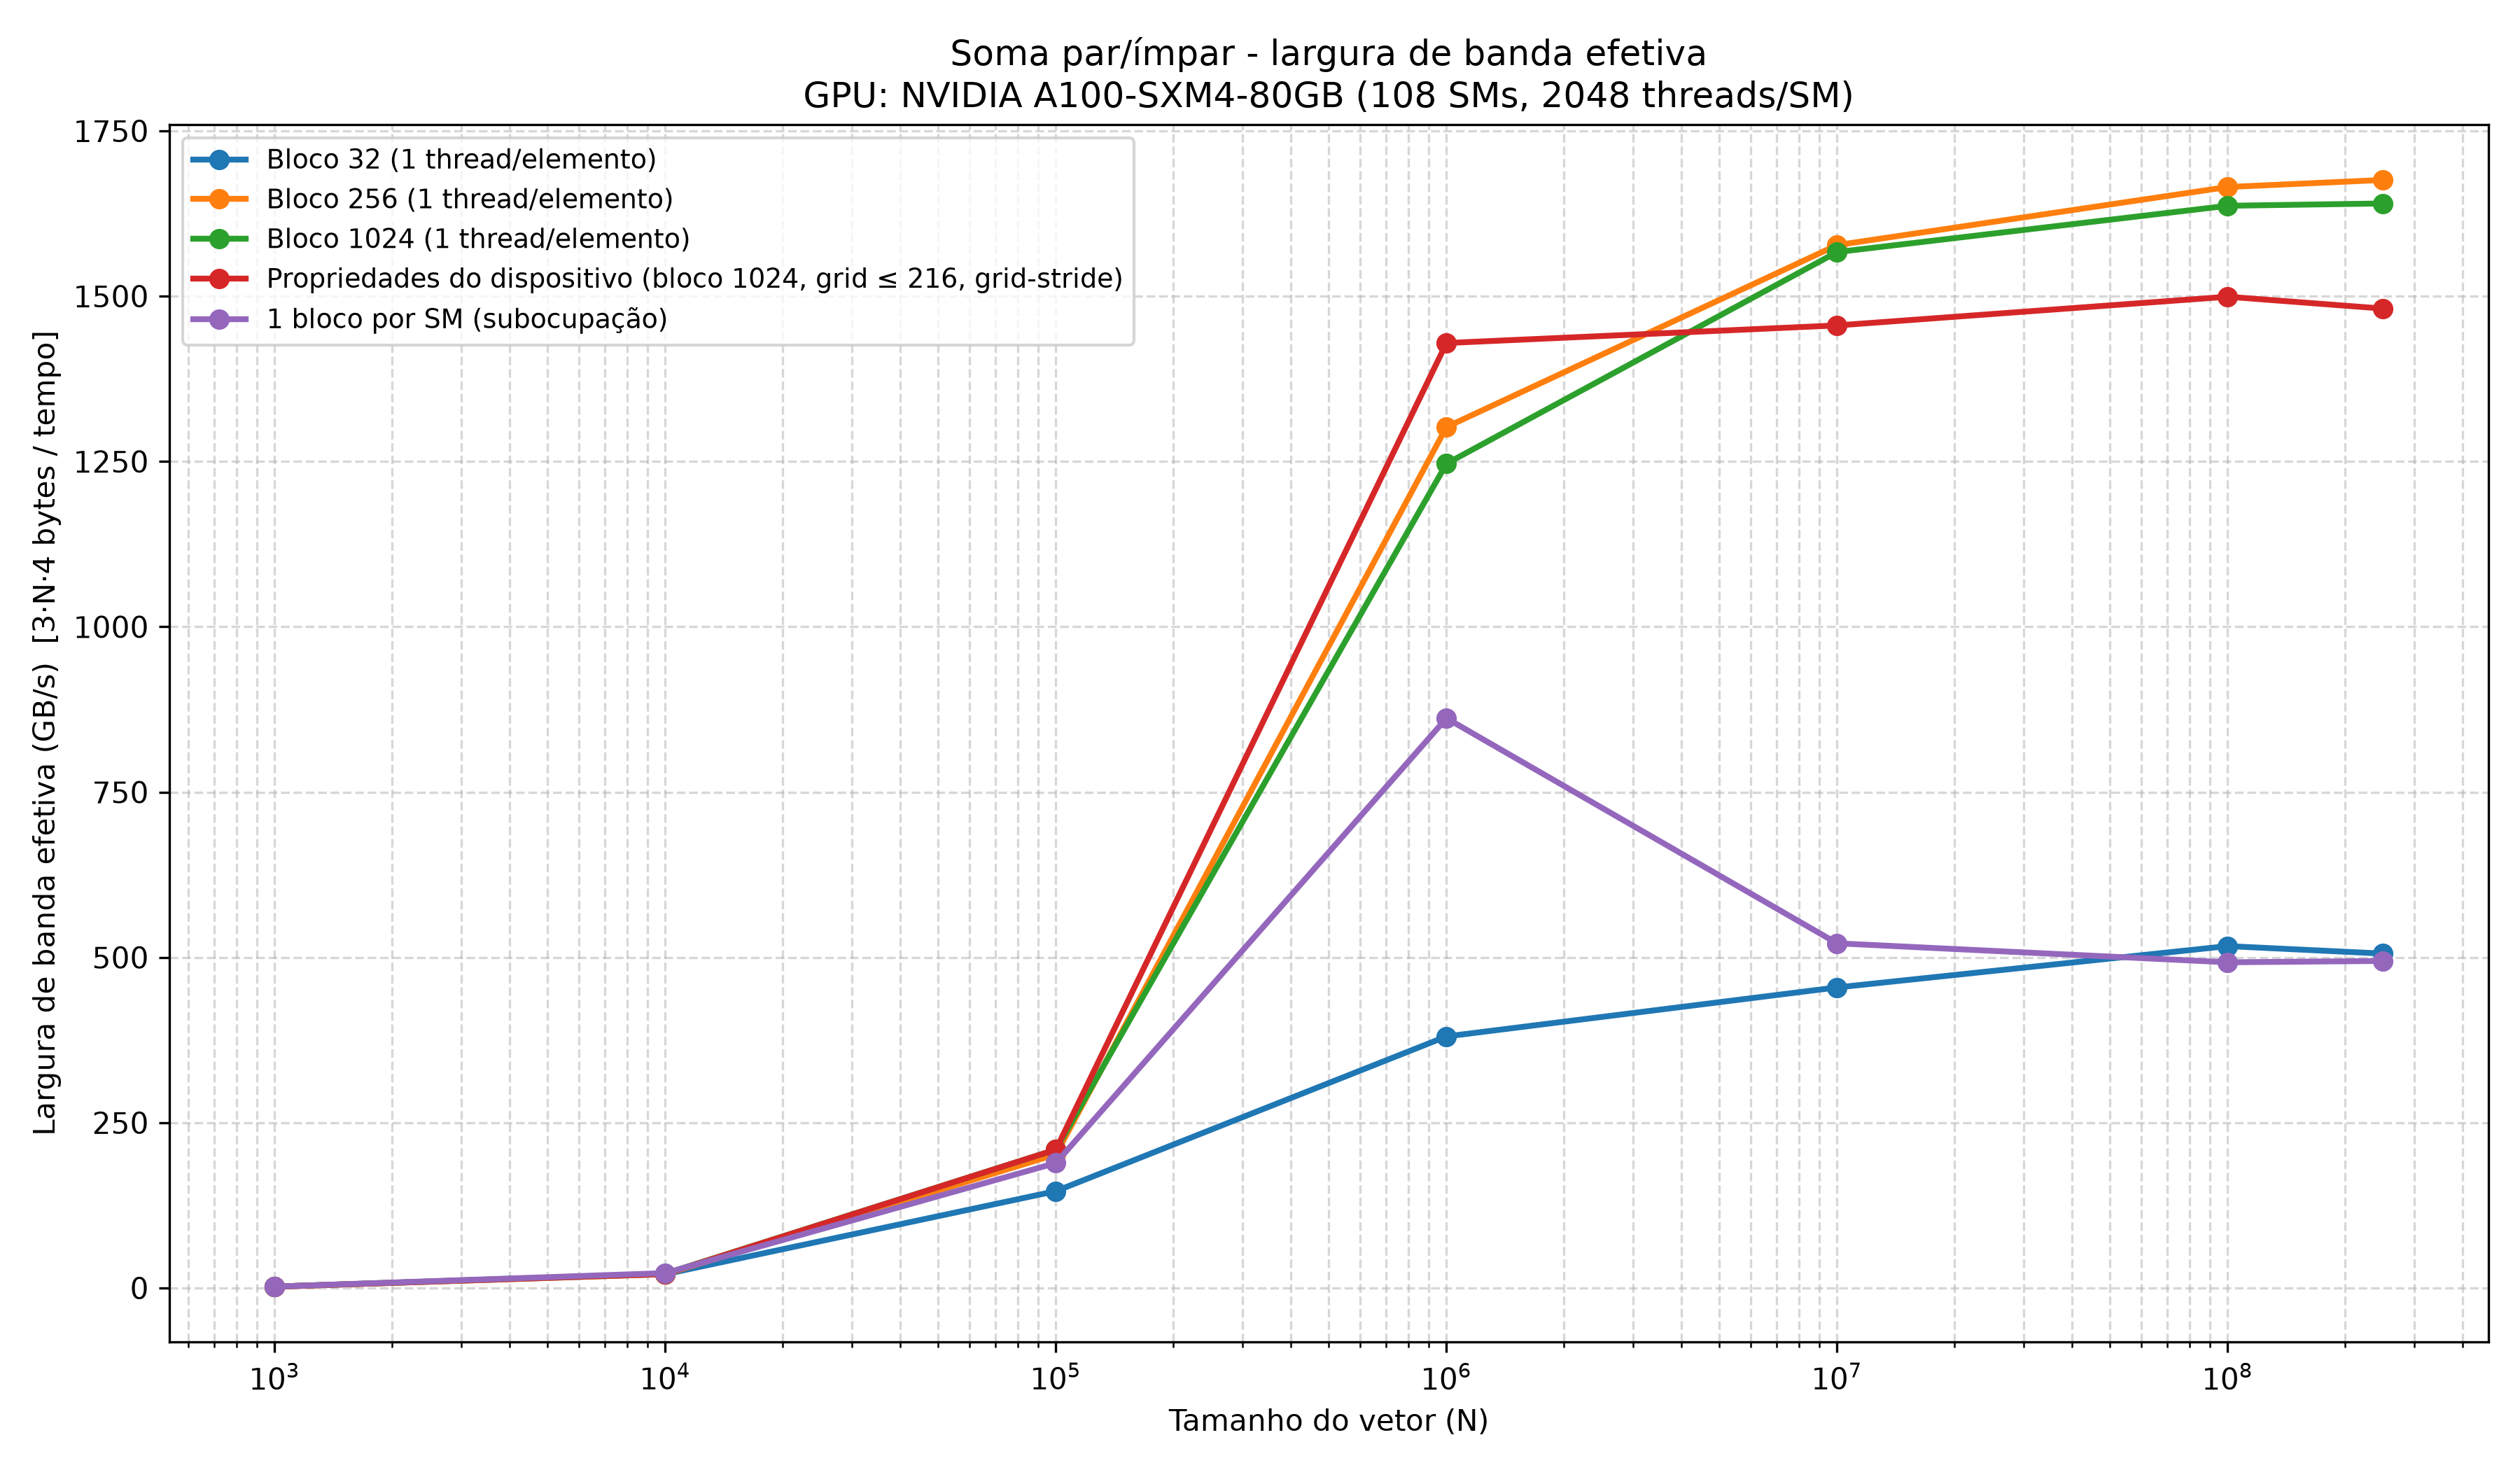
\includegraphics[width=\linewidth]{Tarefa16/tarefa16_banda.png}
			\caption{Tarefa 16 -- Largura de banda efetiva ($3 \cdot N \cdot 4$ bytes / tempo) alcançada por cada configuração em função do tamanho do vetor.}
		\end{figure}
		\begin{figure}[H]
			\centering
			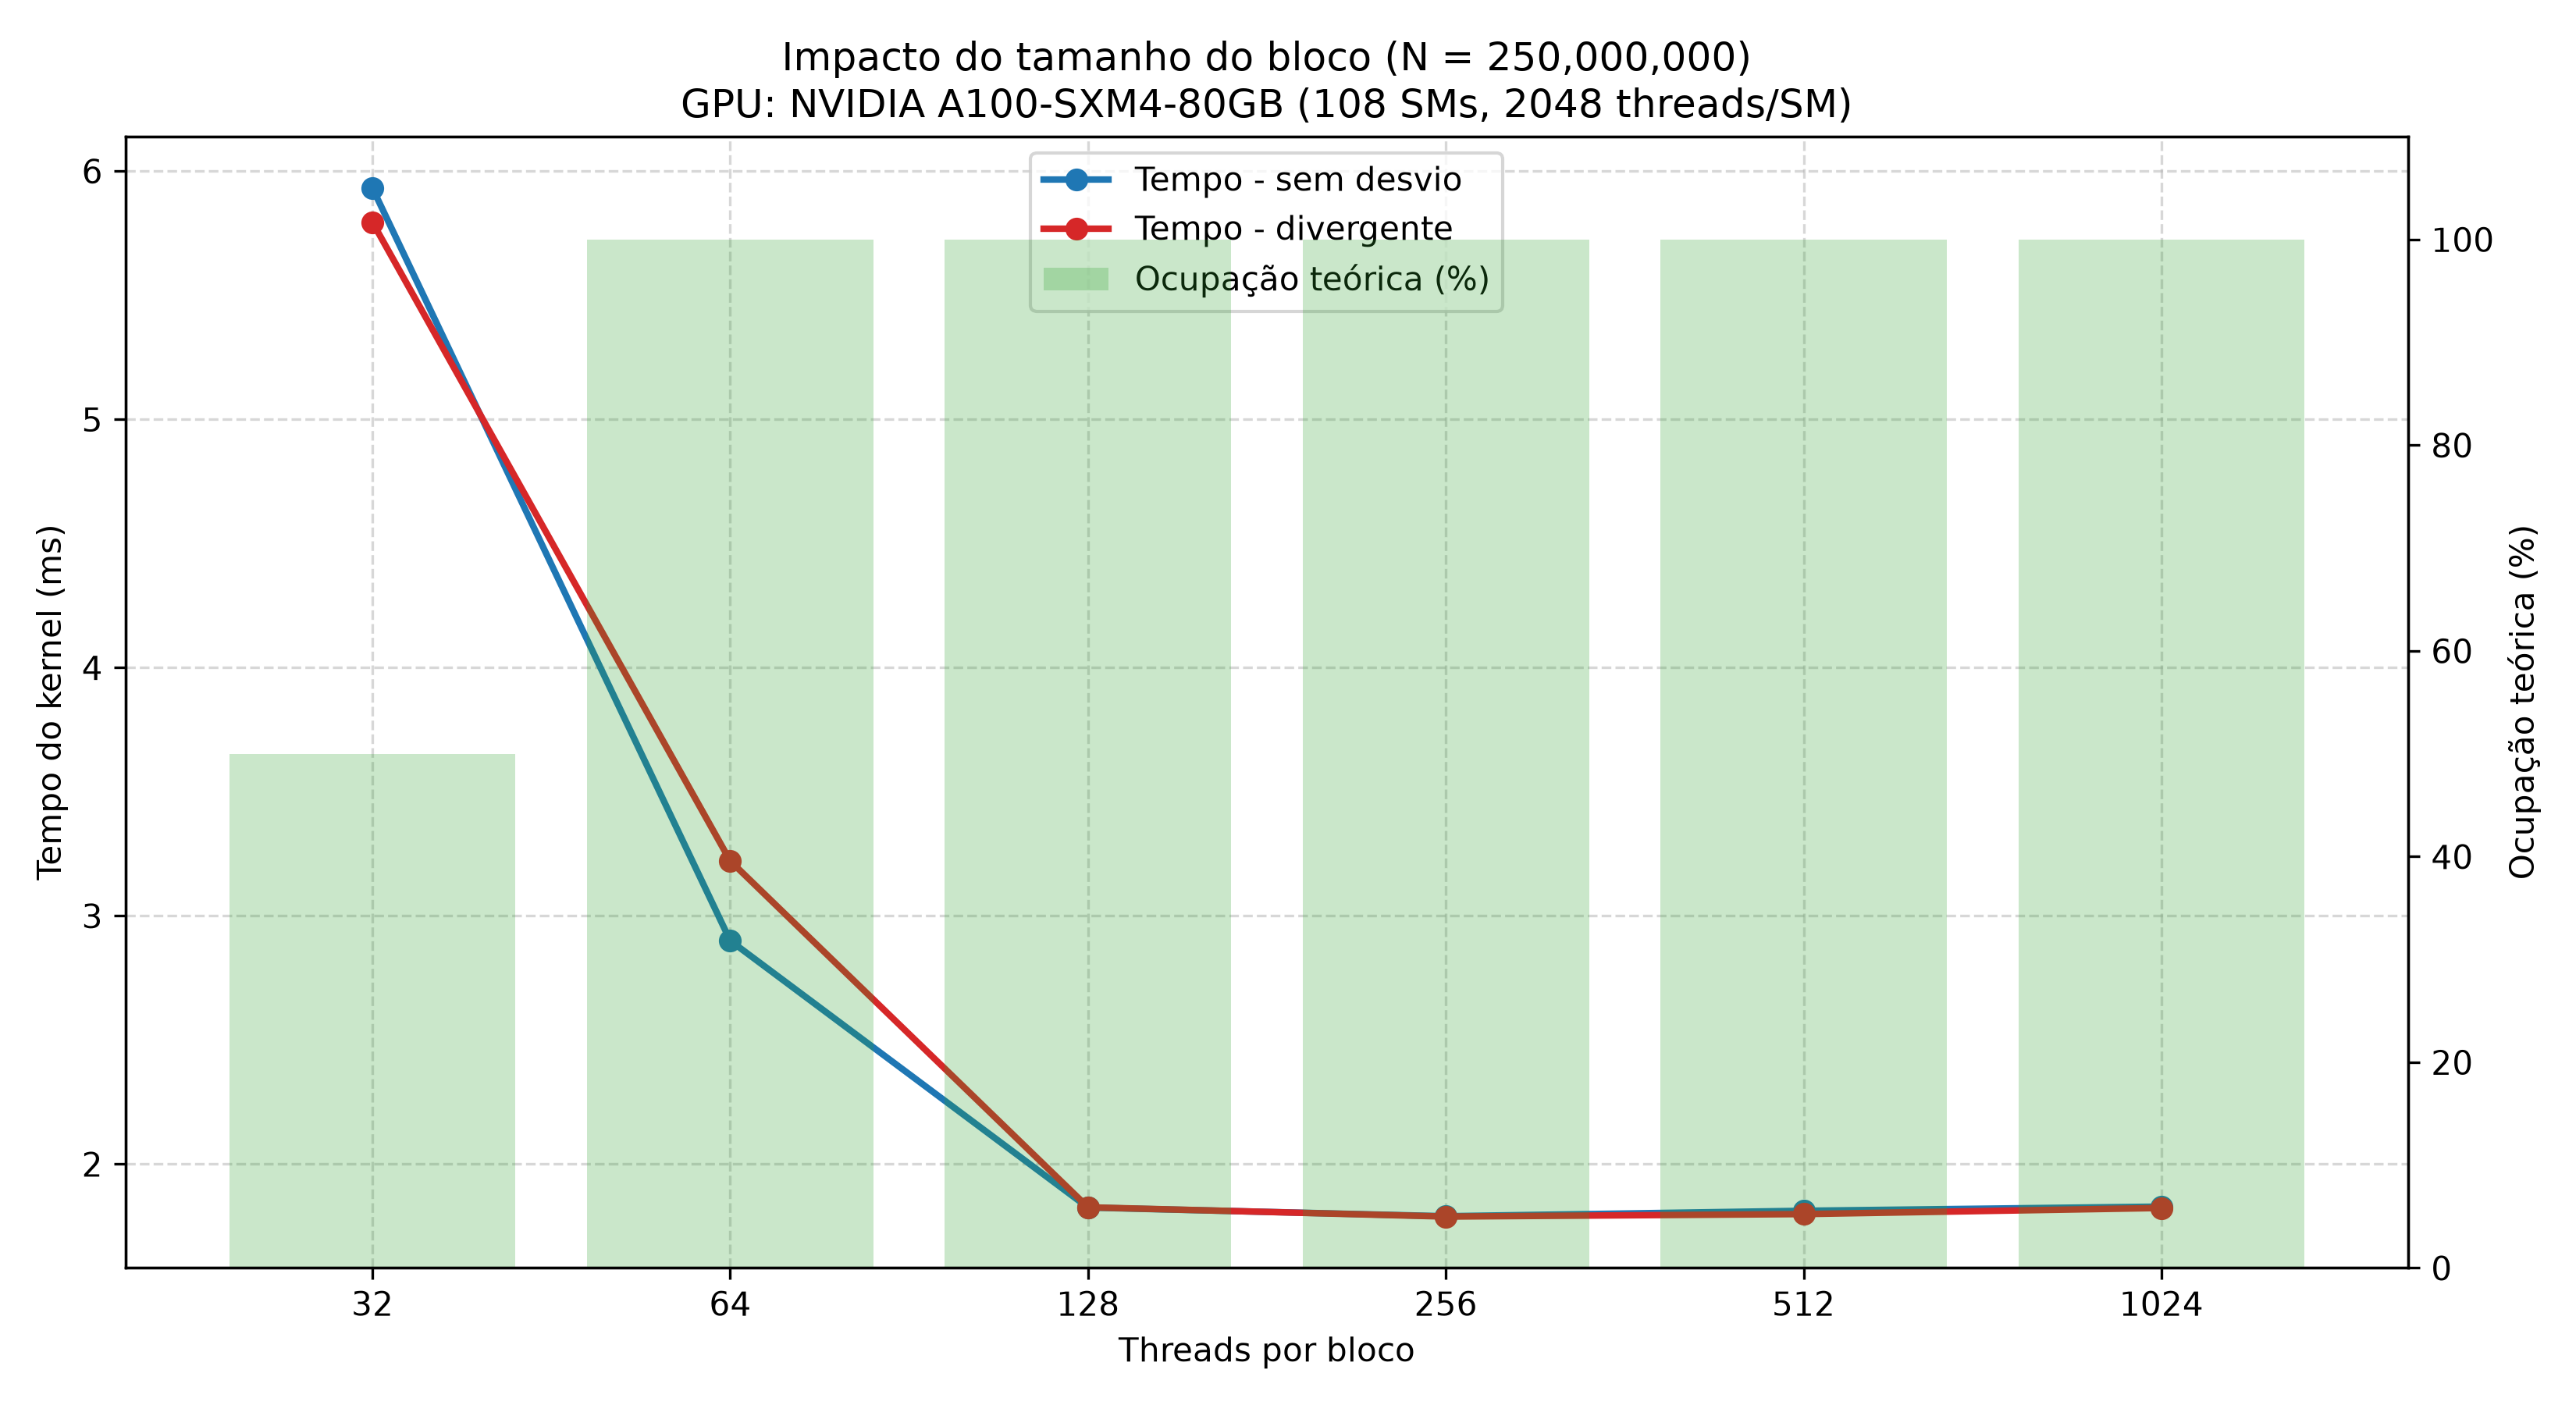
\includegraphics[width=\linewidth]{Tarefa16/tarefa16_blocos.png}
			\caption{Tarefa 16 -- Para o maior vetor: tempo do kernel (com e sem desvio) e ocupação teórica dos SMs em função do número de threads por bloco.}
		\end{figure}
		\begin{figure}[H]
			\centering
			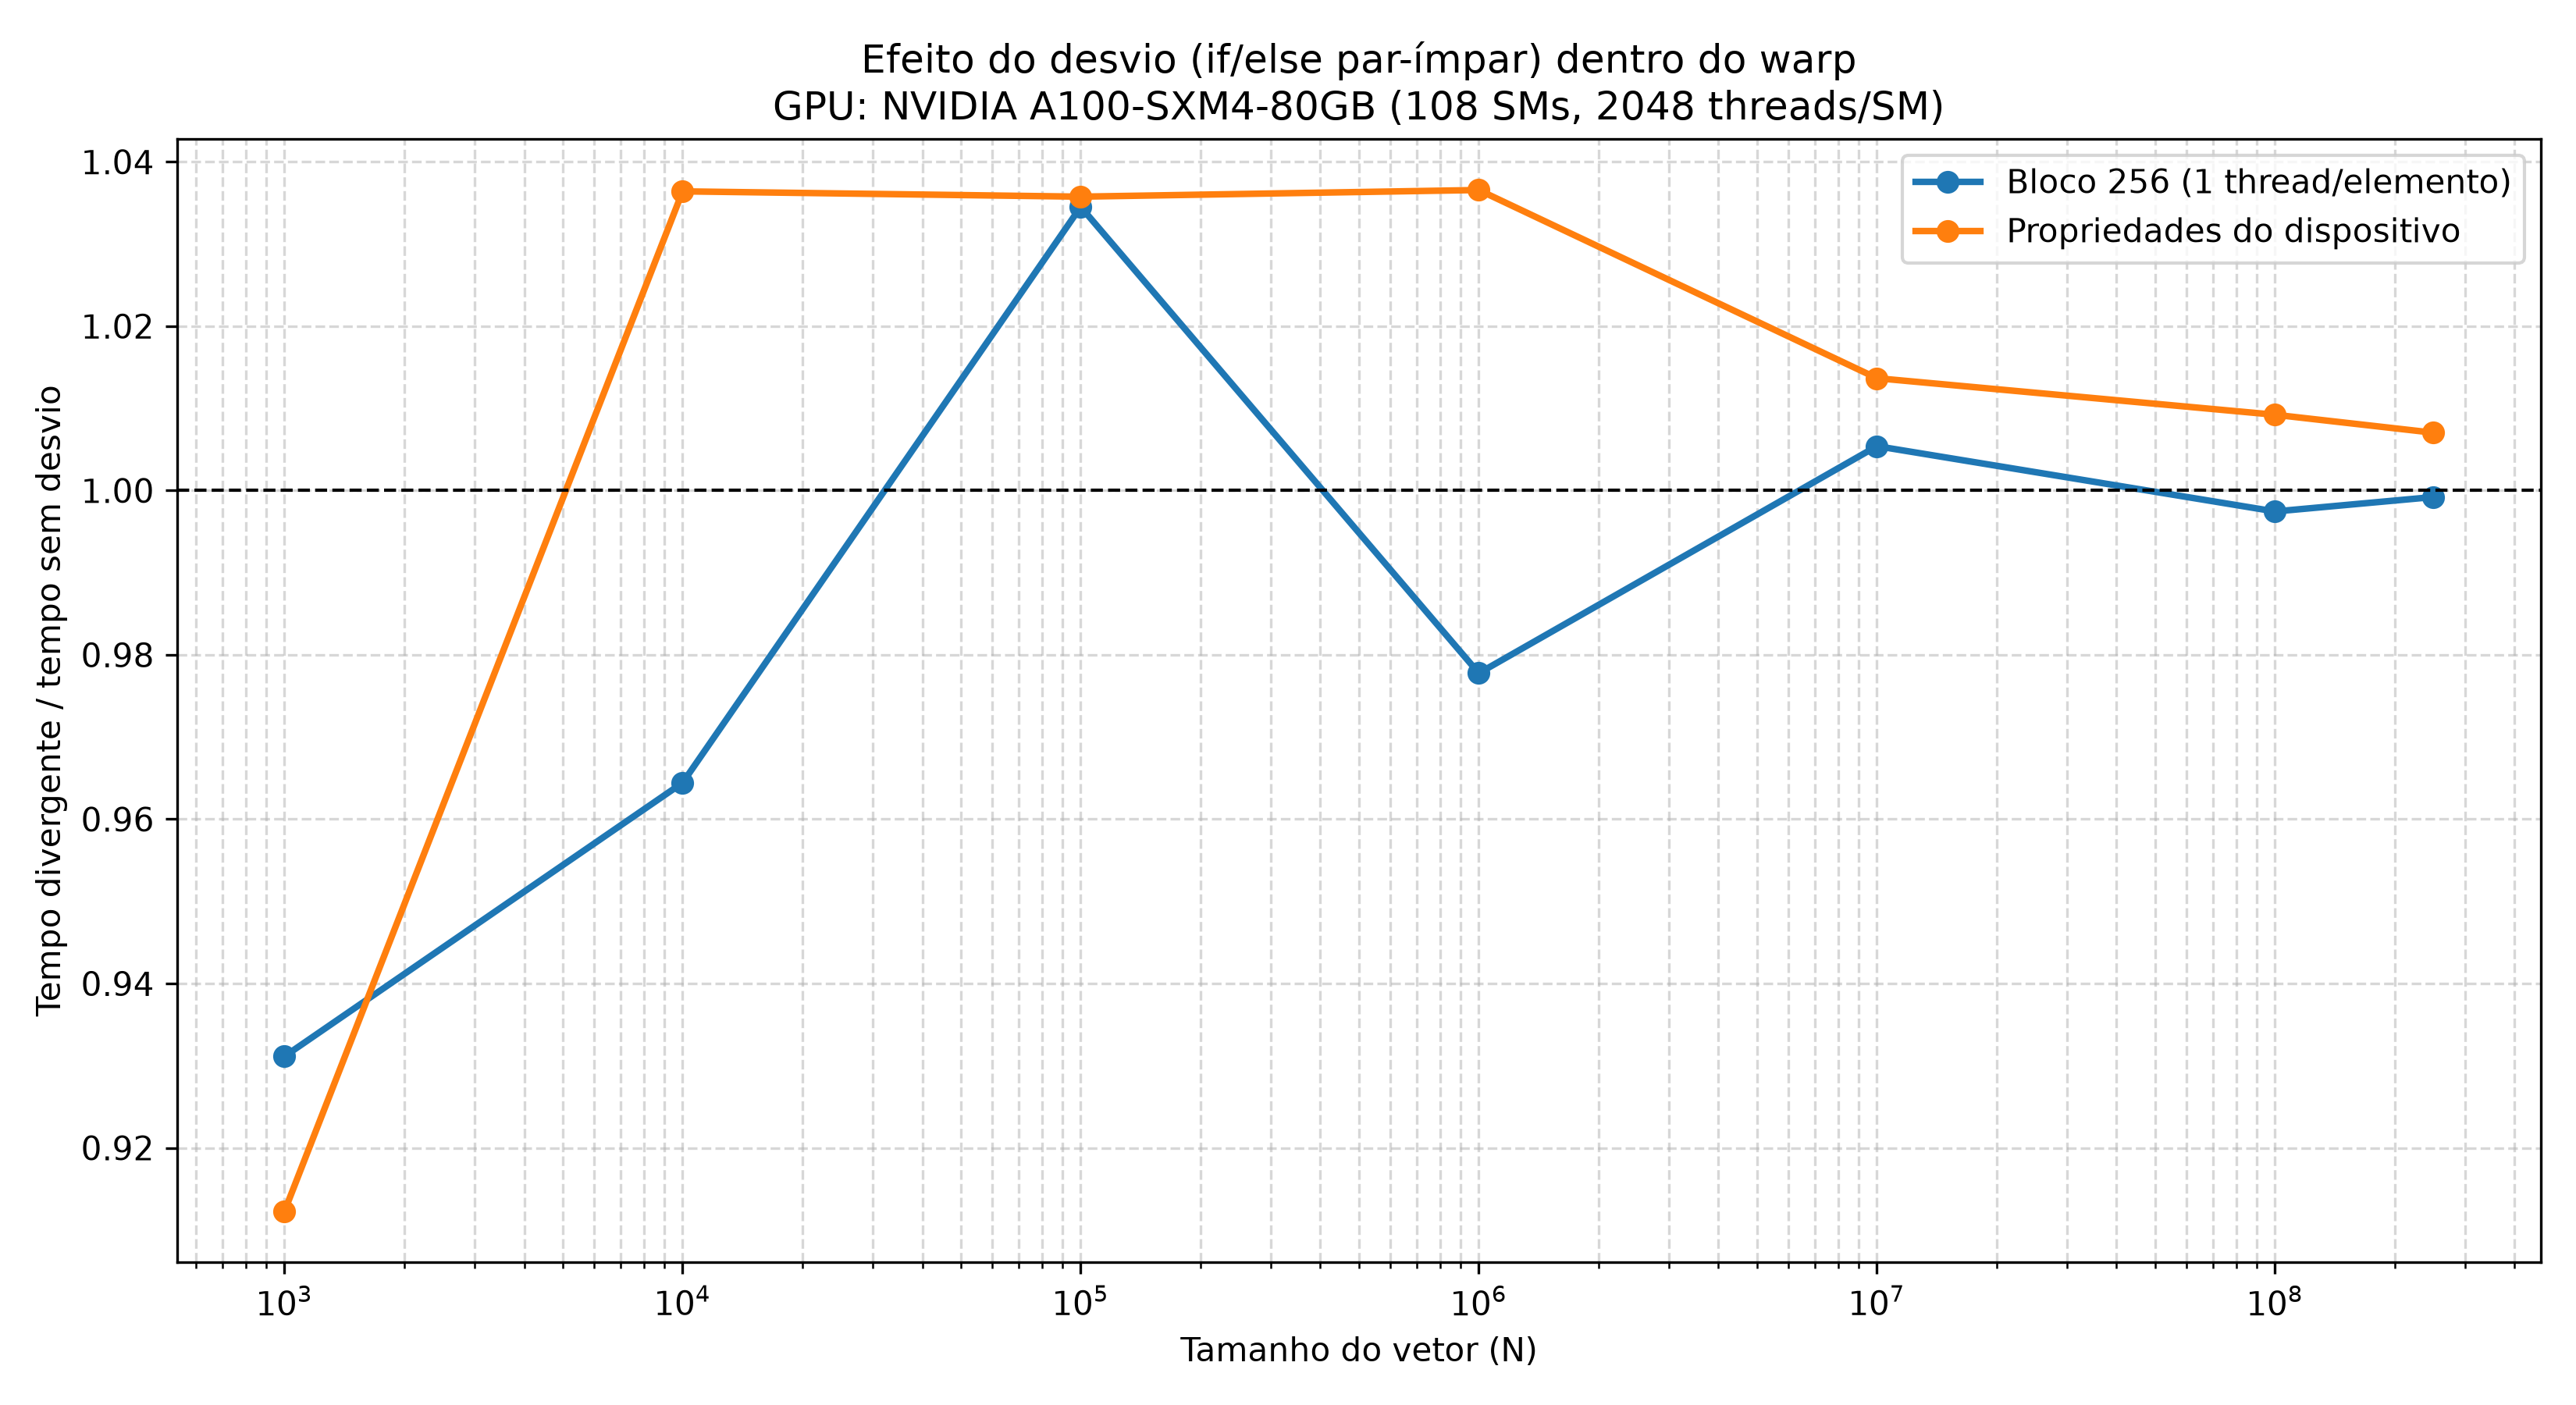
\includegraphics[width=\linewidth]{Tarefa16/tarefa16_divergencia.png}
			\caption{Tarefa 16 -- Razão entre os tempos do kernel com desvio (\texttt{if/else} par/ímpar, divergência no warp) e do kernel sem desvio (\textit{branch-free}).}
		\end{figure}
		\subsection{\subtTres}
		\begin{lstlisting}[language=c]
		\end{lstlisting}
		
	\newpage
		\onehalfspacing
		\section{TAREFA 17}
		\subsection{\subtUm}
		\par{Implementar versões de um programa de envio de mensagens entre processos com MPI, onde o processo 0 envia uma mensagem para o processo 1, que imediatamente responde com o mesmo conteúdo.
		
		Medir o tempo total de execução de múltiplas trocas consecutivas de mensagens, registrando os tempos para diferentes tamanhos de conteúdo.
		
		Analisar com gráficos o comportamento identificado, identificando onde a latência domina e onde a largura de banda se torna o fator principal, explicando cada implementação e função.}
		\subsection{\subtDois}
		\par{Texto}
		\begin{figure}[H]
			\centering
			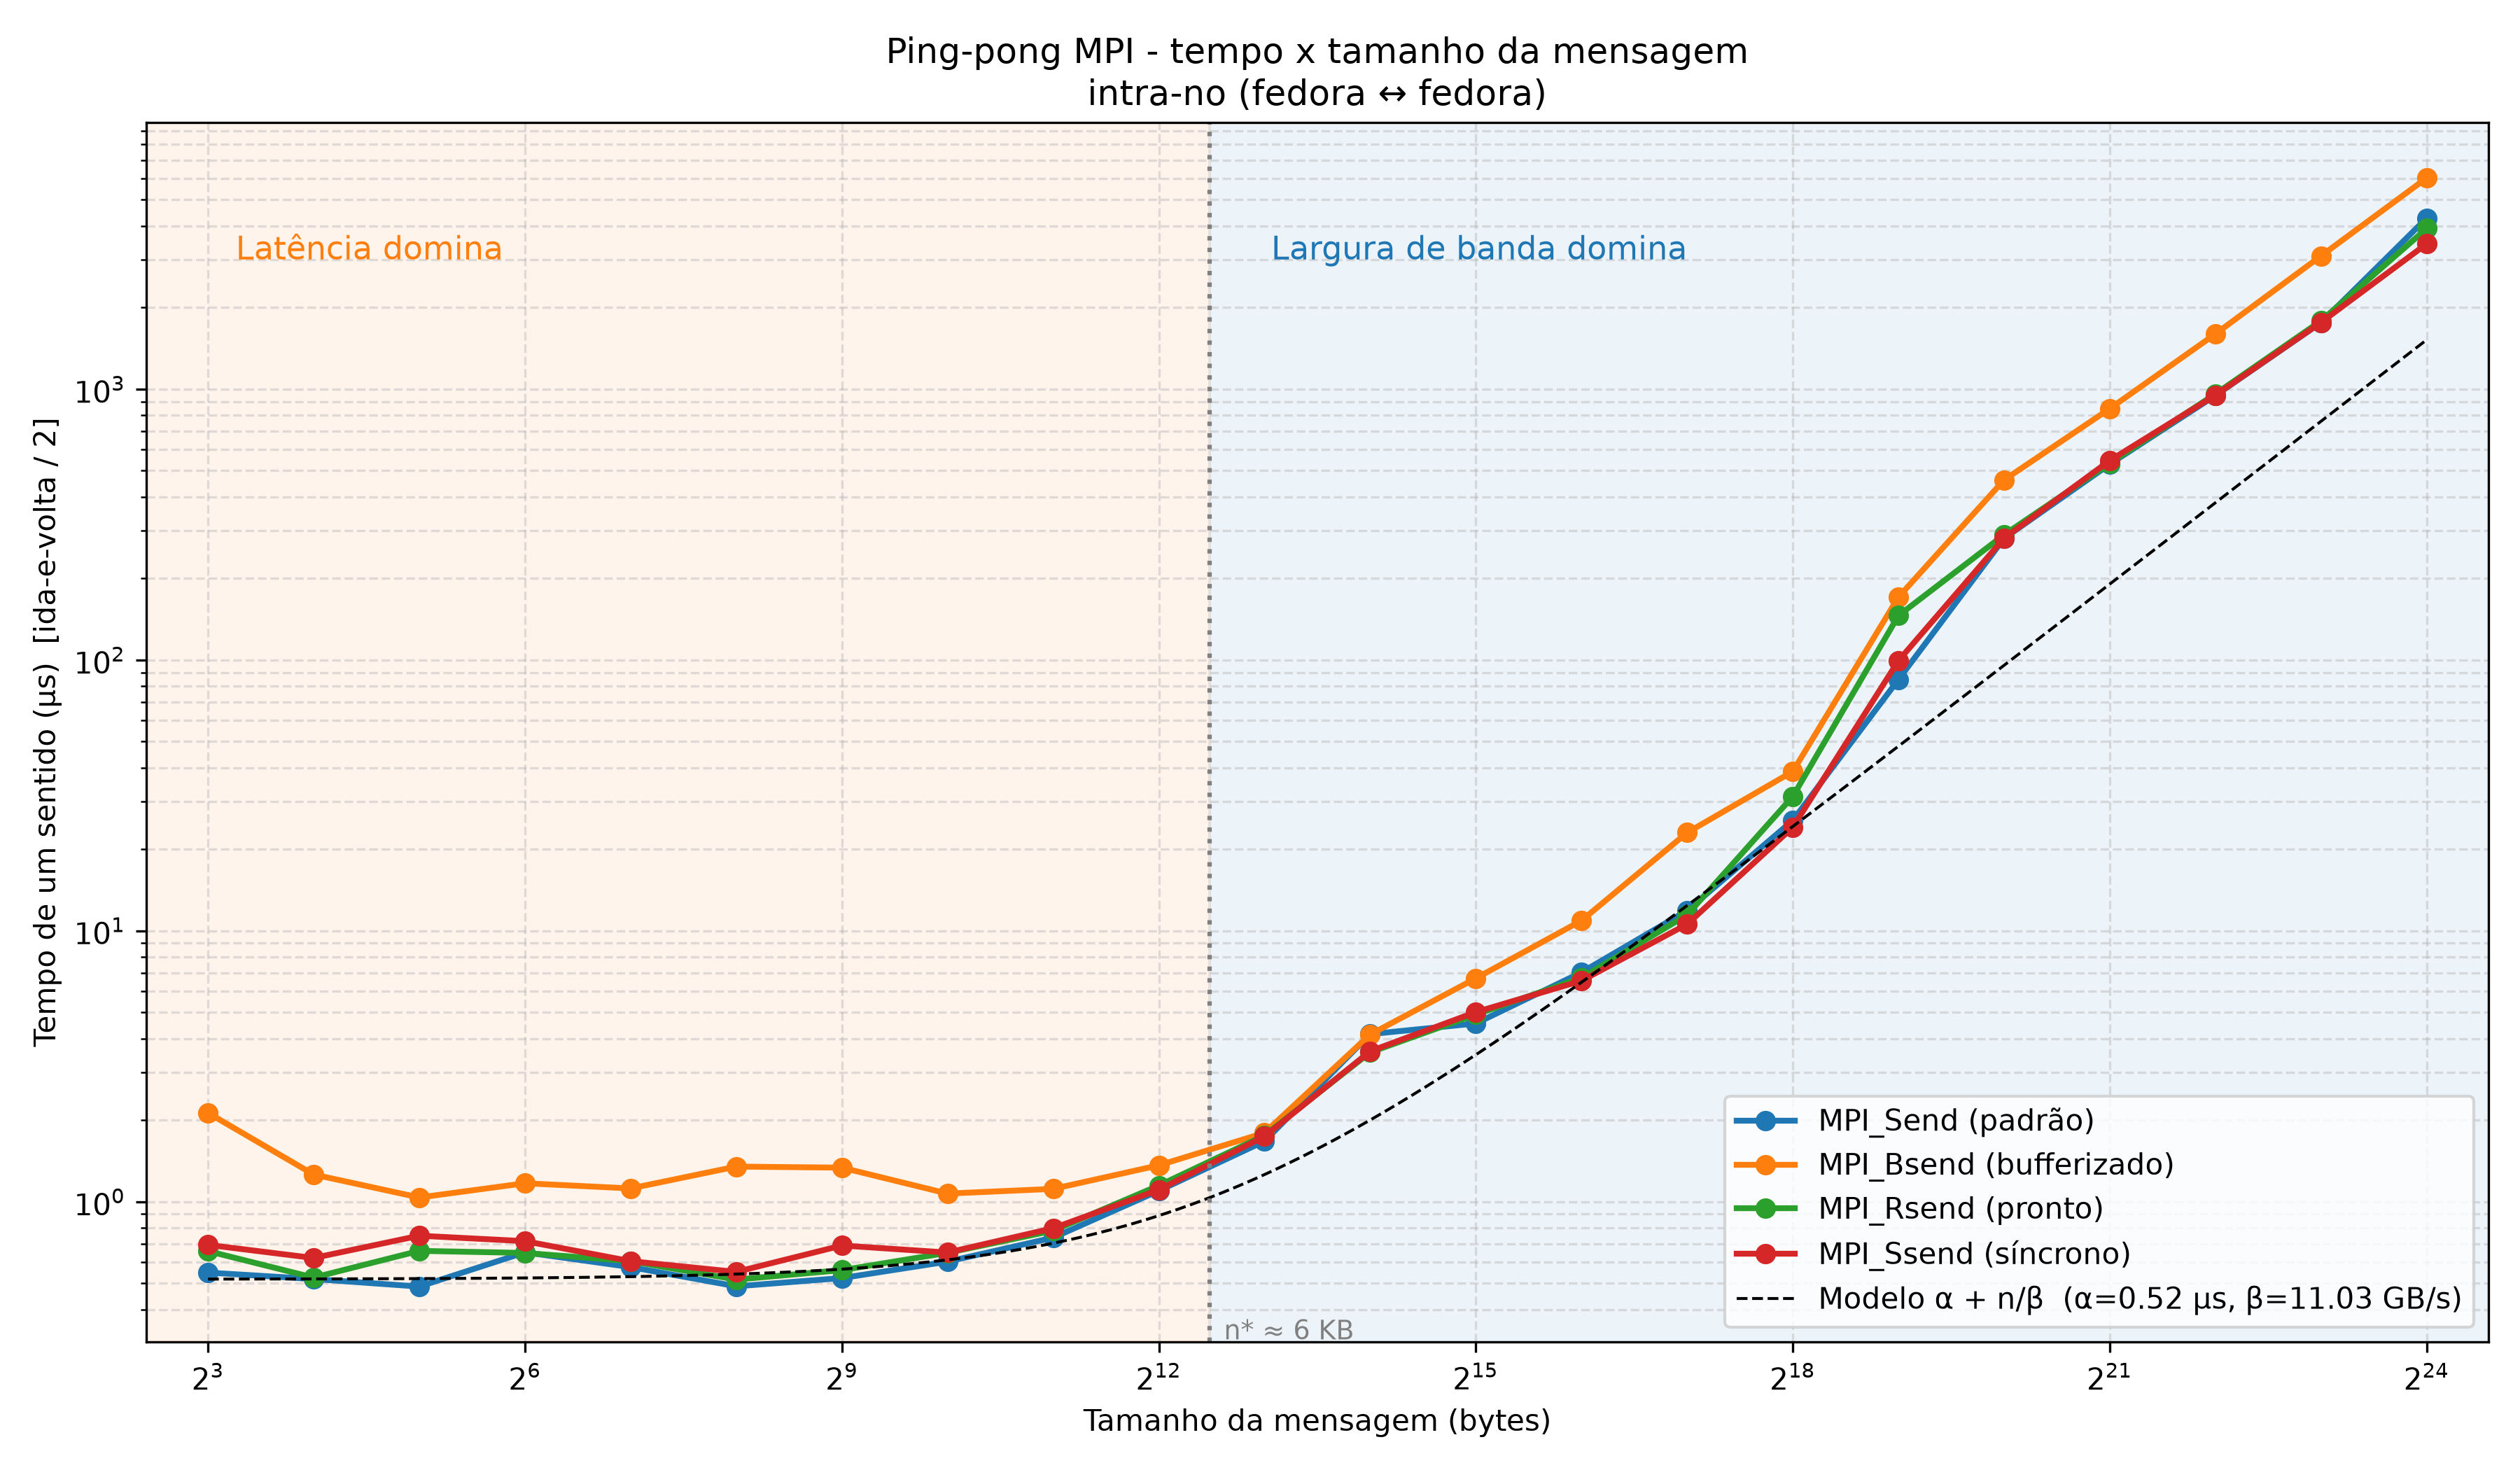
\includegraphics[width=\linewidth]{Tarefa17/tarefa17_tempo.png}
			\caption{Tarefa 17 -- Tempo de um sentido do ping-pong em função do tamanho da mensagem para \texttt{MPI\_Send}, \texttt{MPI\_Bsend}, \texttt{MPI\_Rsend} e \texttt{MPI\_Ssend}, com o modelo $t(n) = \alpha + n/\beta$ e as regiões dominadas pela latência e pela largura de banda.}
		\end{figure}
		\begin{figure}[H]
			\centering
			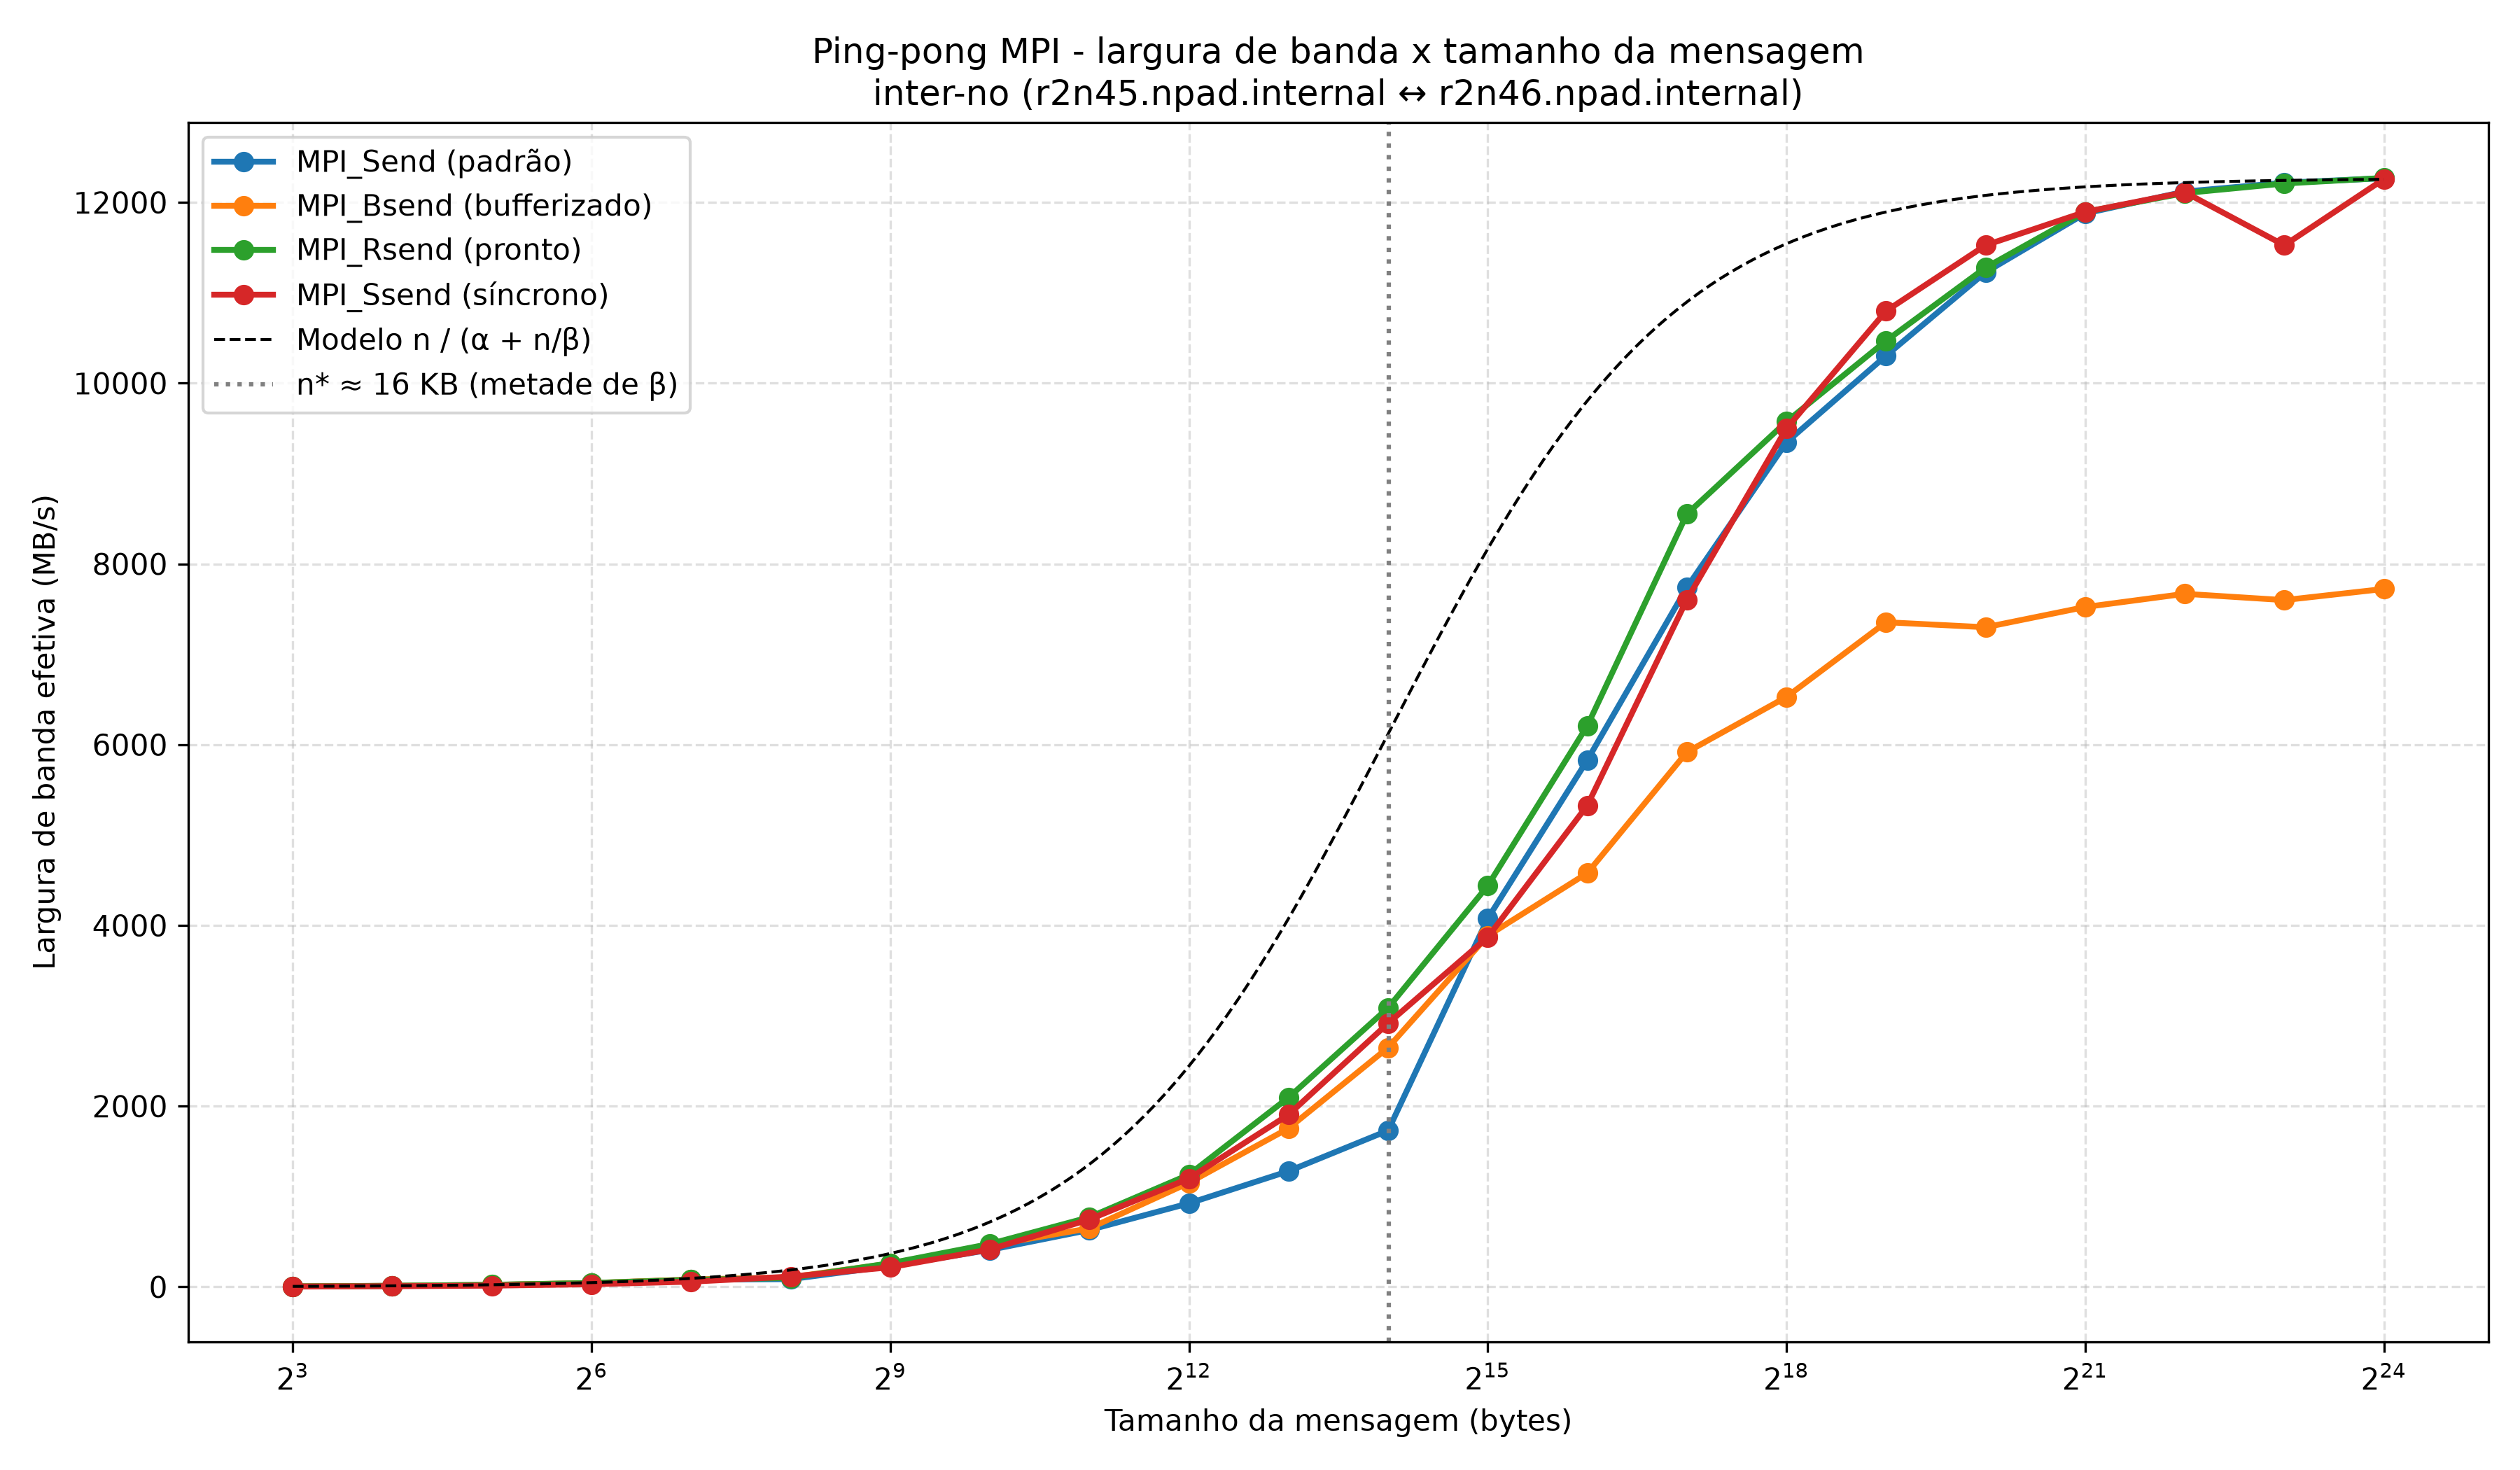
\includegraphics[width=\linewidth]{Tarefa17/tarefa17_banda.png}
			\caption{Tarefa 17 -- Largura de banda efetiva em função do tamanho da mensagem para cada modo de envio; a linha pontilhada marca o tamanho $n^* = \alpha\beta$, no qual se atinge metade da banda assintótica.}
		\end{figure}
		\subsection{\subtTres}
		\begin{lstlisting}[language=c]
		\end{lstlisting}
		
	\newpage
		\onehalfspacing
		\section{TAREFA 18}
		\subsection{\subtUm}
		\par{Adaptar o código de propagação de onda para que cada fonte sísmica seja processada de forma independente por um processo MPI através de um escalonador dinâmico com o modelo Master-Worker.
		
		O processo líder deve enviar um struct com a posição da fonte sísmica pra ser processada. Cada trabalhador processa os dados recebidos e enviar uma mensagem ao líder indicando o resultado, que irá então atualizar a informação para atribuir uma nova tarefa ao trabalhador.
		
		Apresentar os resultados, variando a quantidade de fontes a serem processadas, analisando o comportamento do escalonador em função da quantidade de tiros.}
		\subsection{\subtDois}
		\par{Texto}
		\begin{figure}[H]
			\centering
			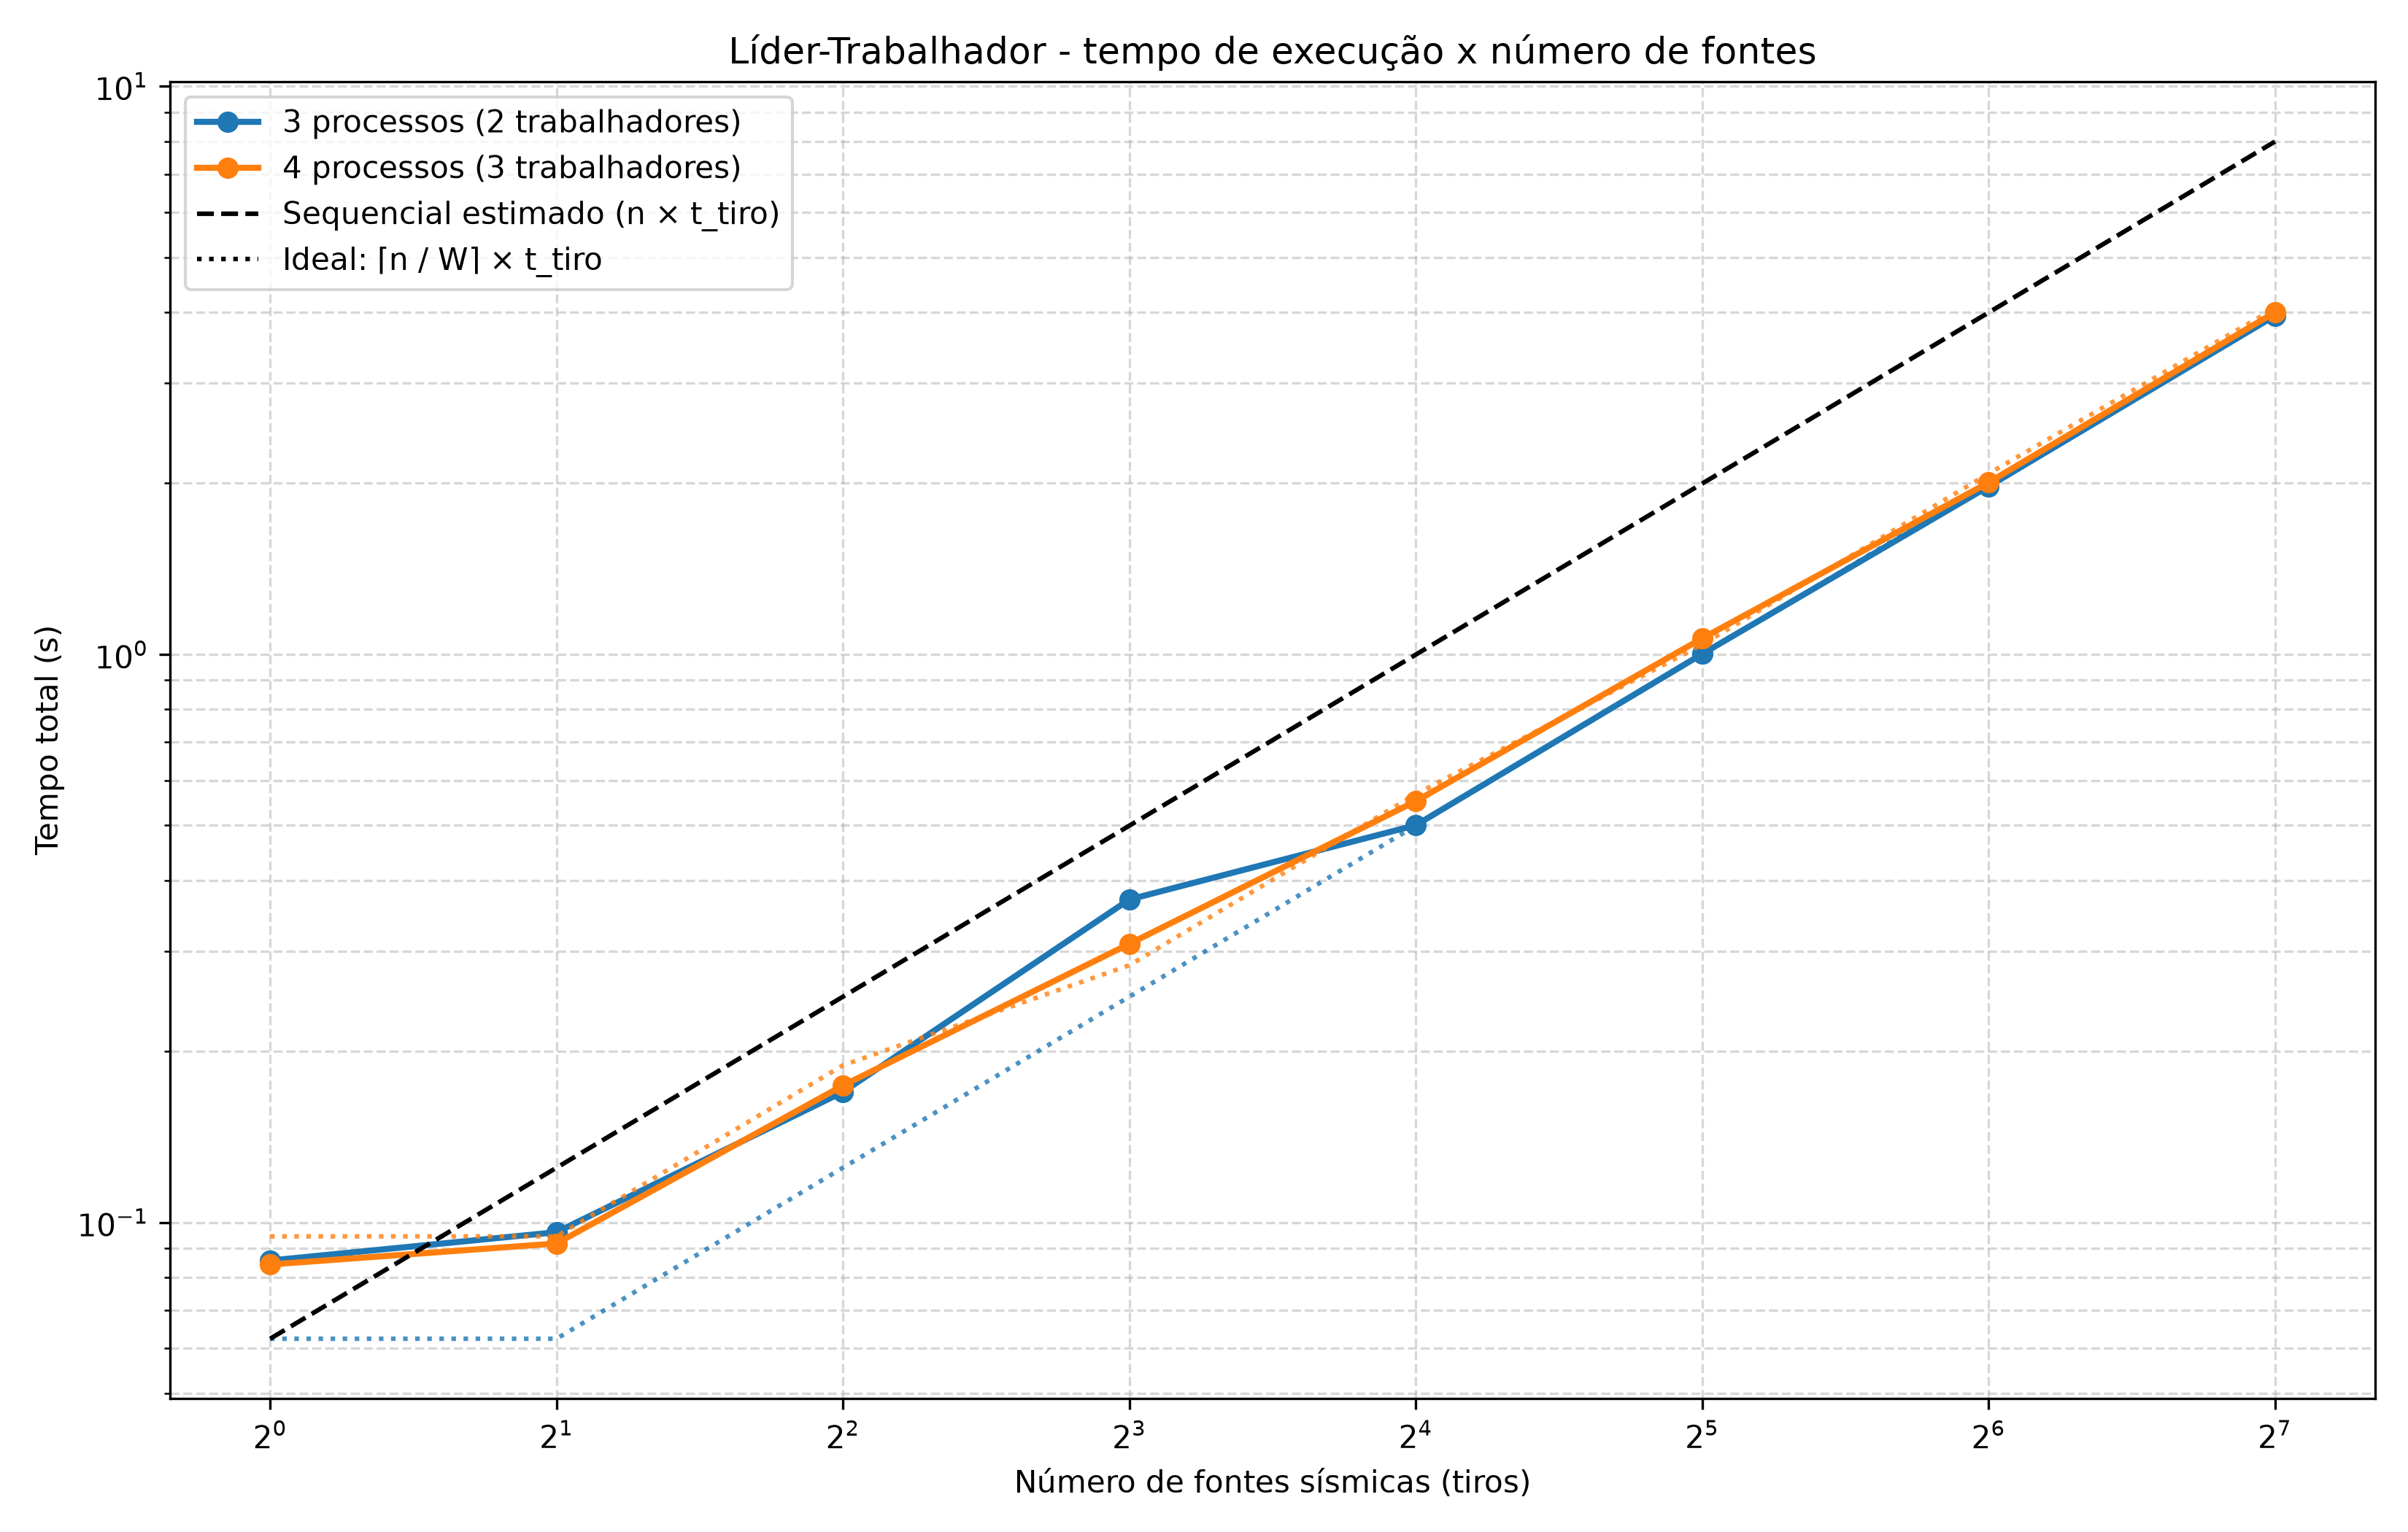
\includegraphics[width=\linewidth]{Tarefa18/tarefa18_tempo.png}
			\caption{Tarefa 18 -- Tempo total do escalonador Líder-Trabalhador em função do número de fontes sísmicas, para cada número de processos, comparado ao tempo sequencial estimado e ao ideal $\lceil n/W \rceil \cdot t_{tiro}$.}
		\end{figure}
		\begin{figure}[H]
			\centering
			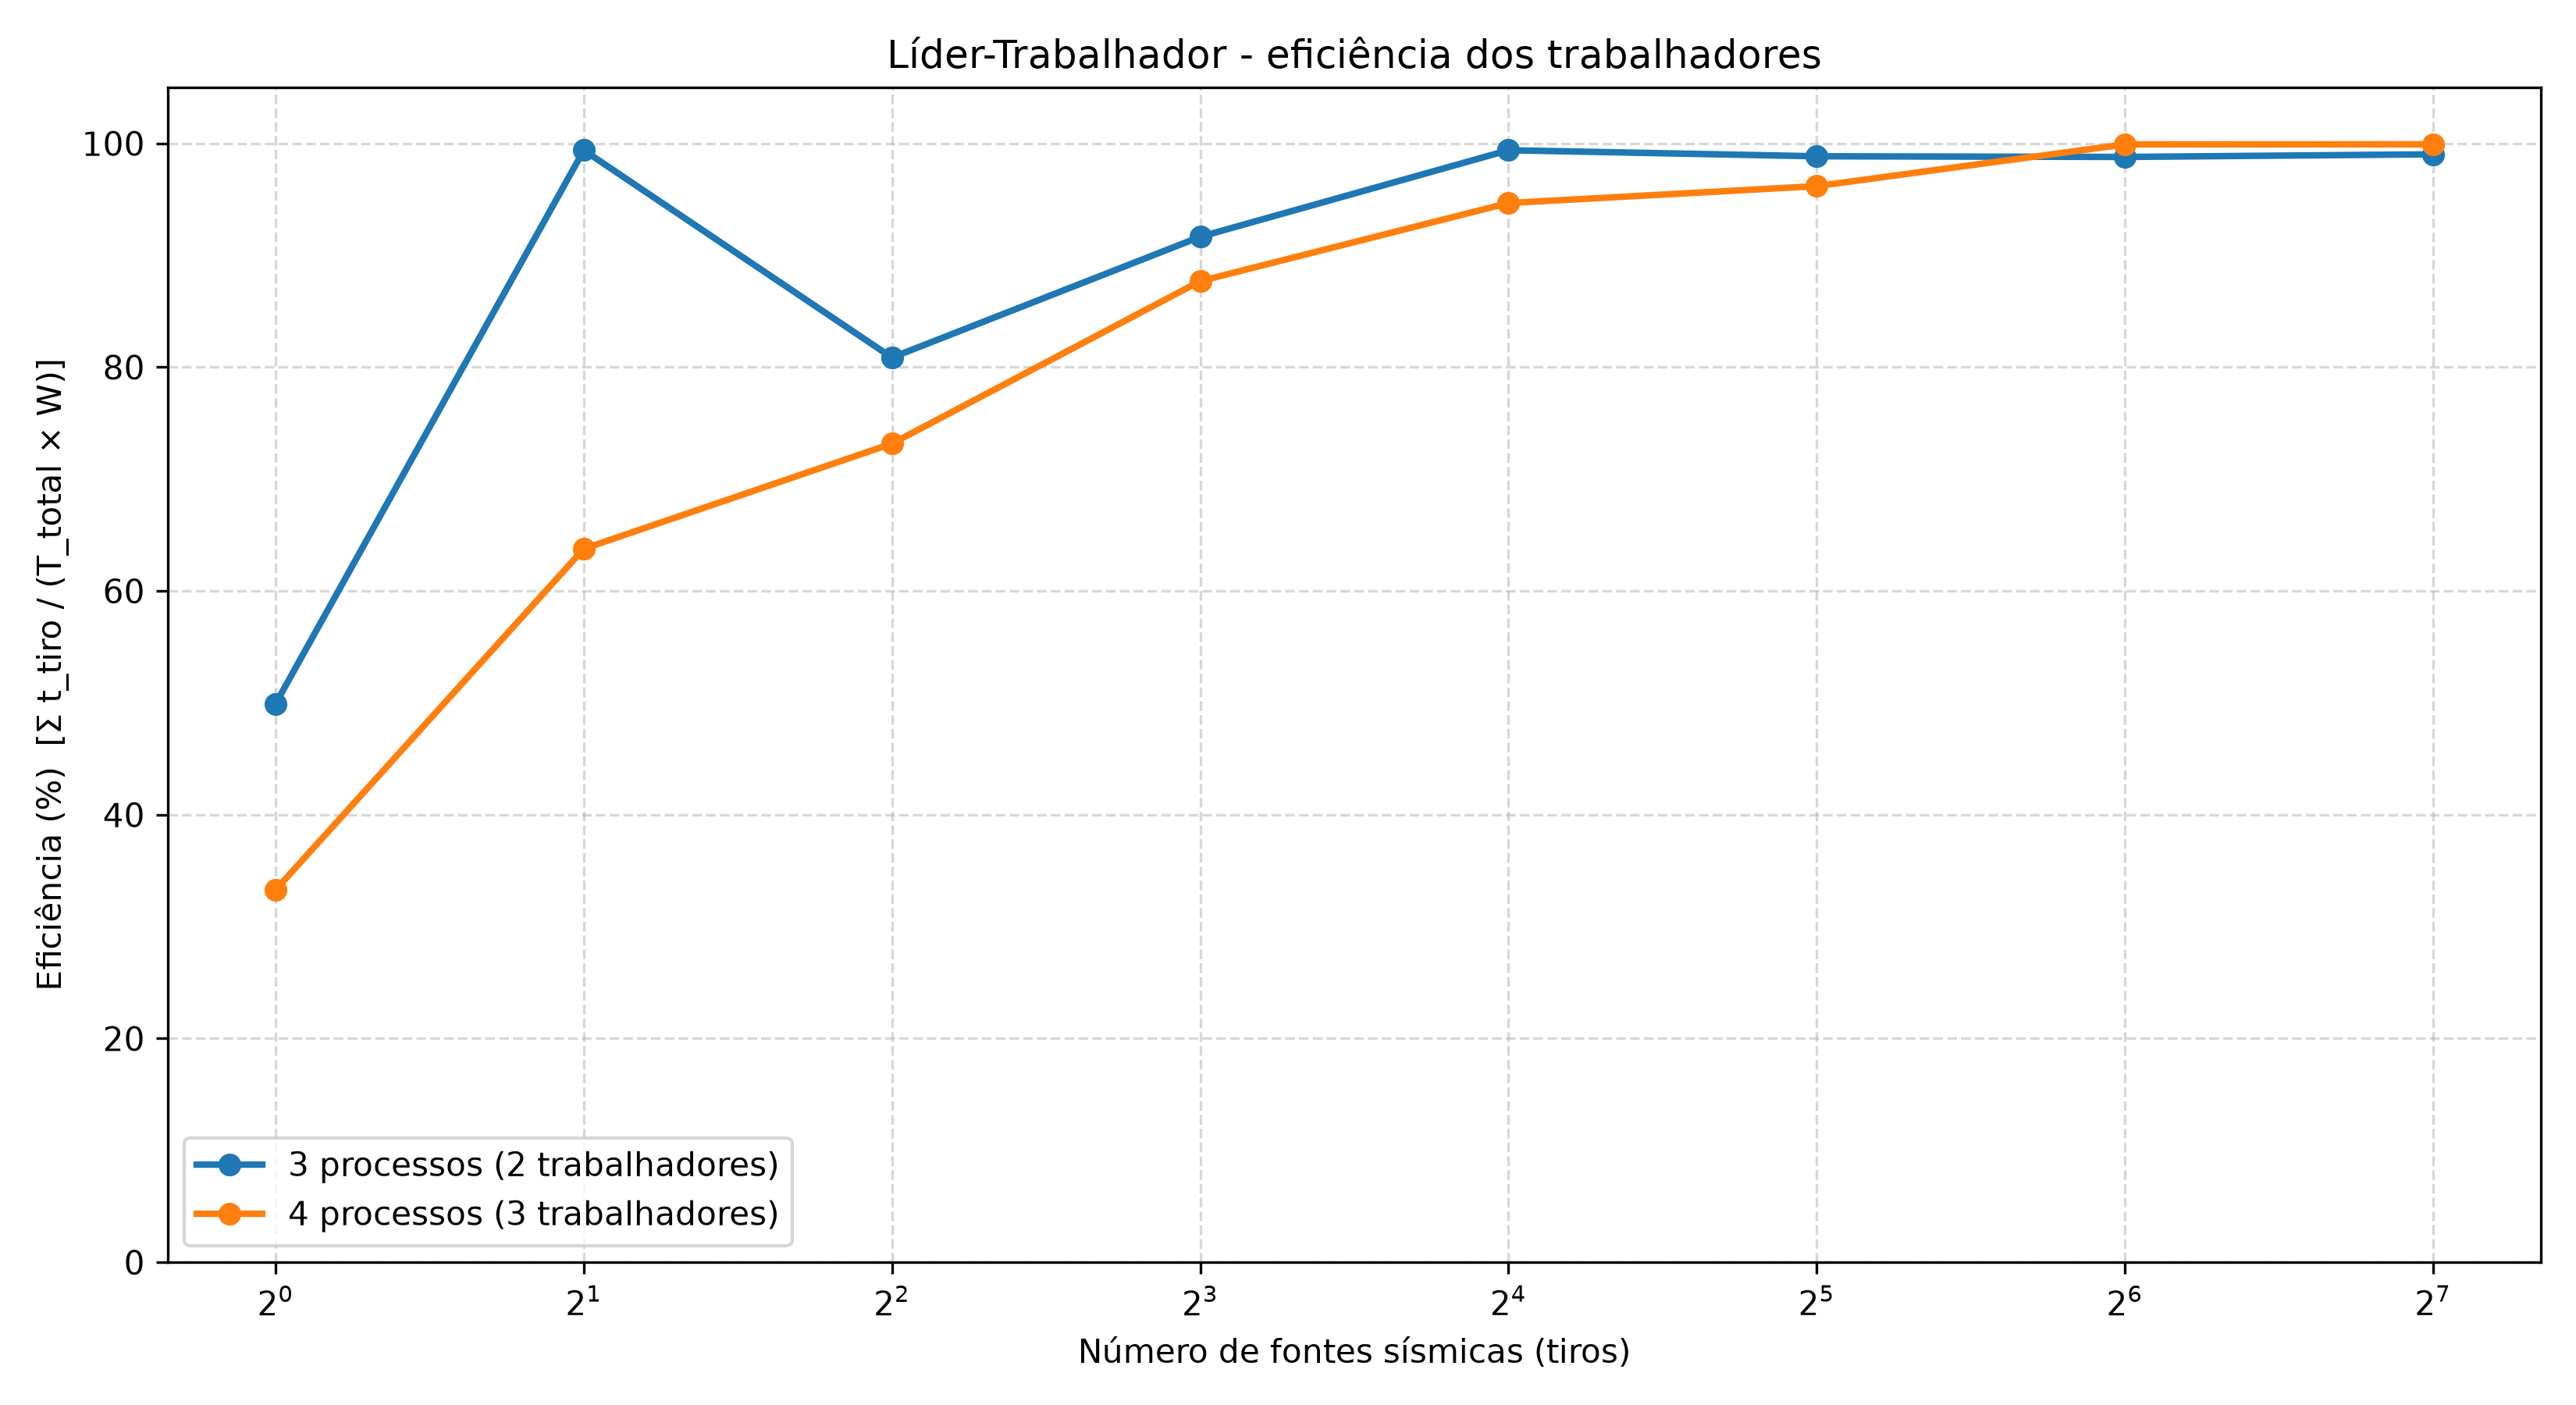
\includegraphics[width=\linewidth]{Tarefa18/tarefa18_eficiencia.png}
			\caption{Tarefa 18 -- Eficiência dos trabalhadores ($\sum t_{tiro} / (T_{total} \cdot W)$) em função do número de fontes sísmicas.}
		\end{figure}
		\begin{figure}[H]
			\centering
			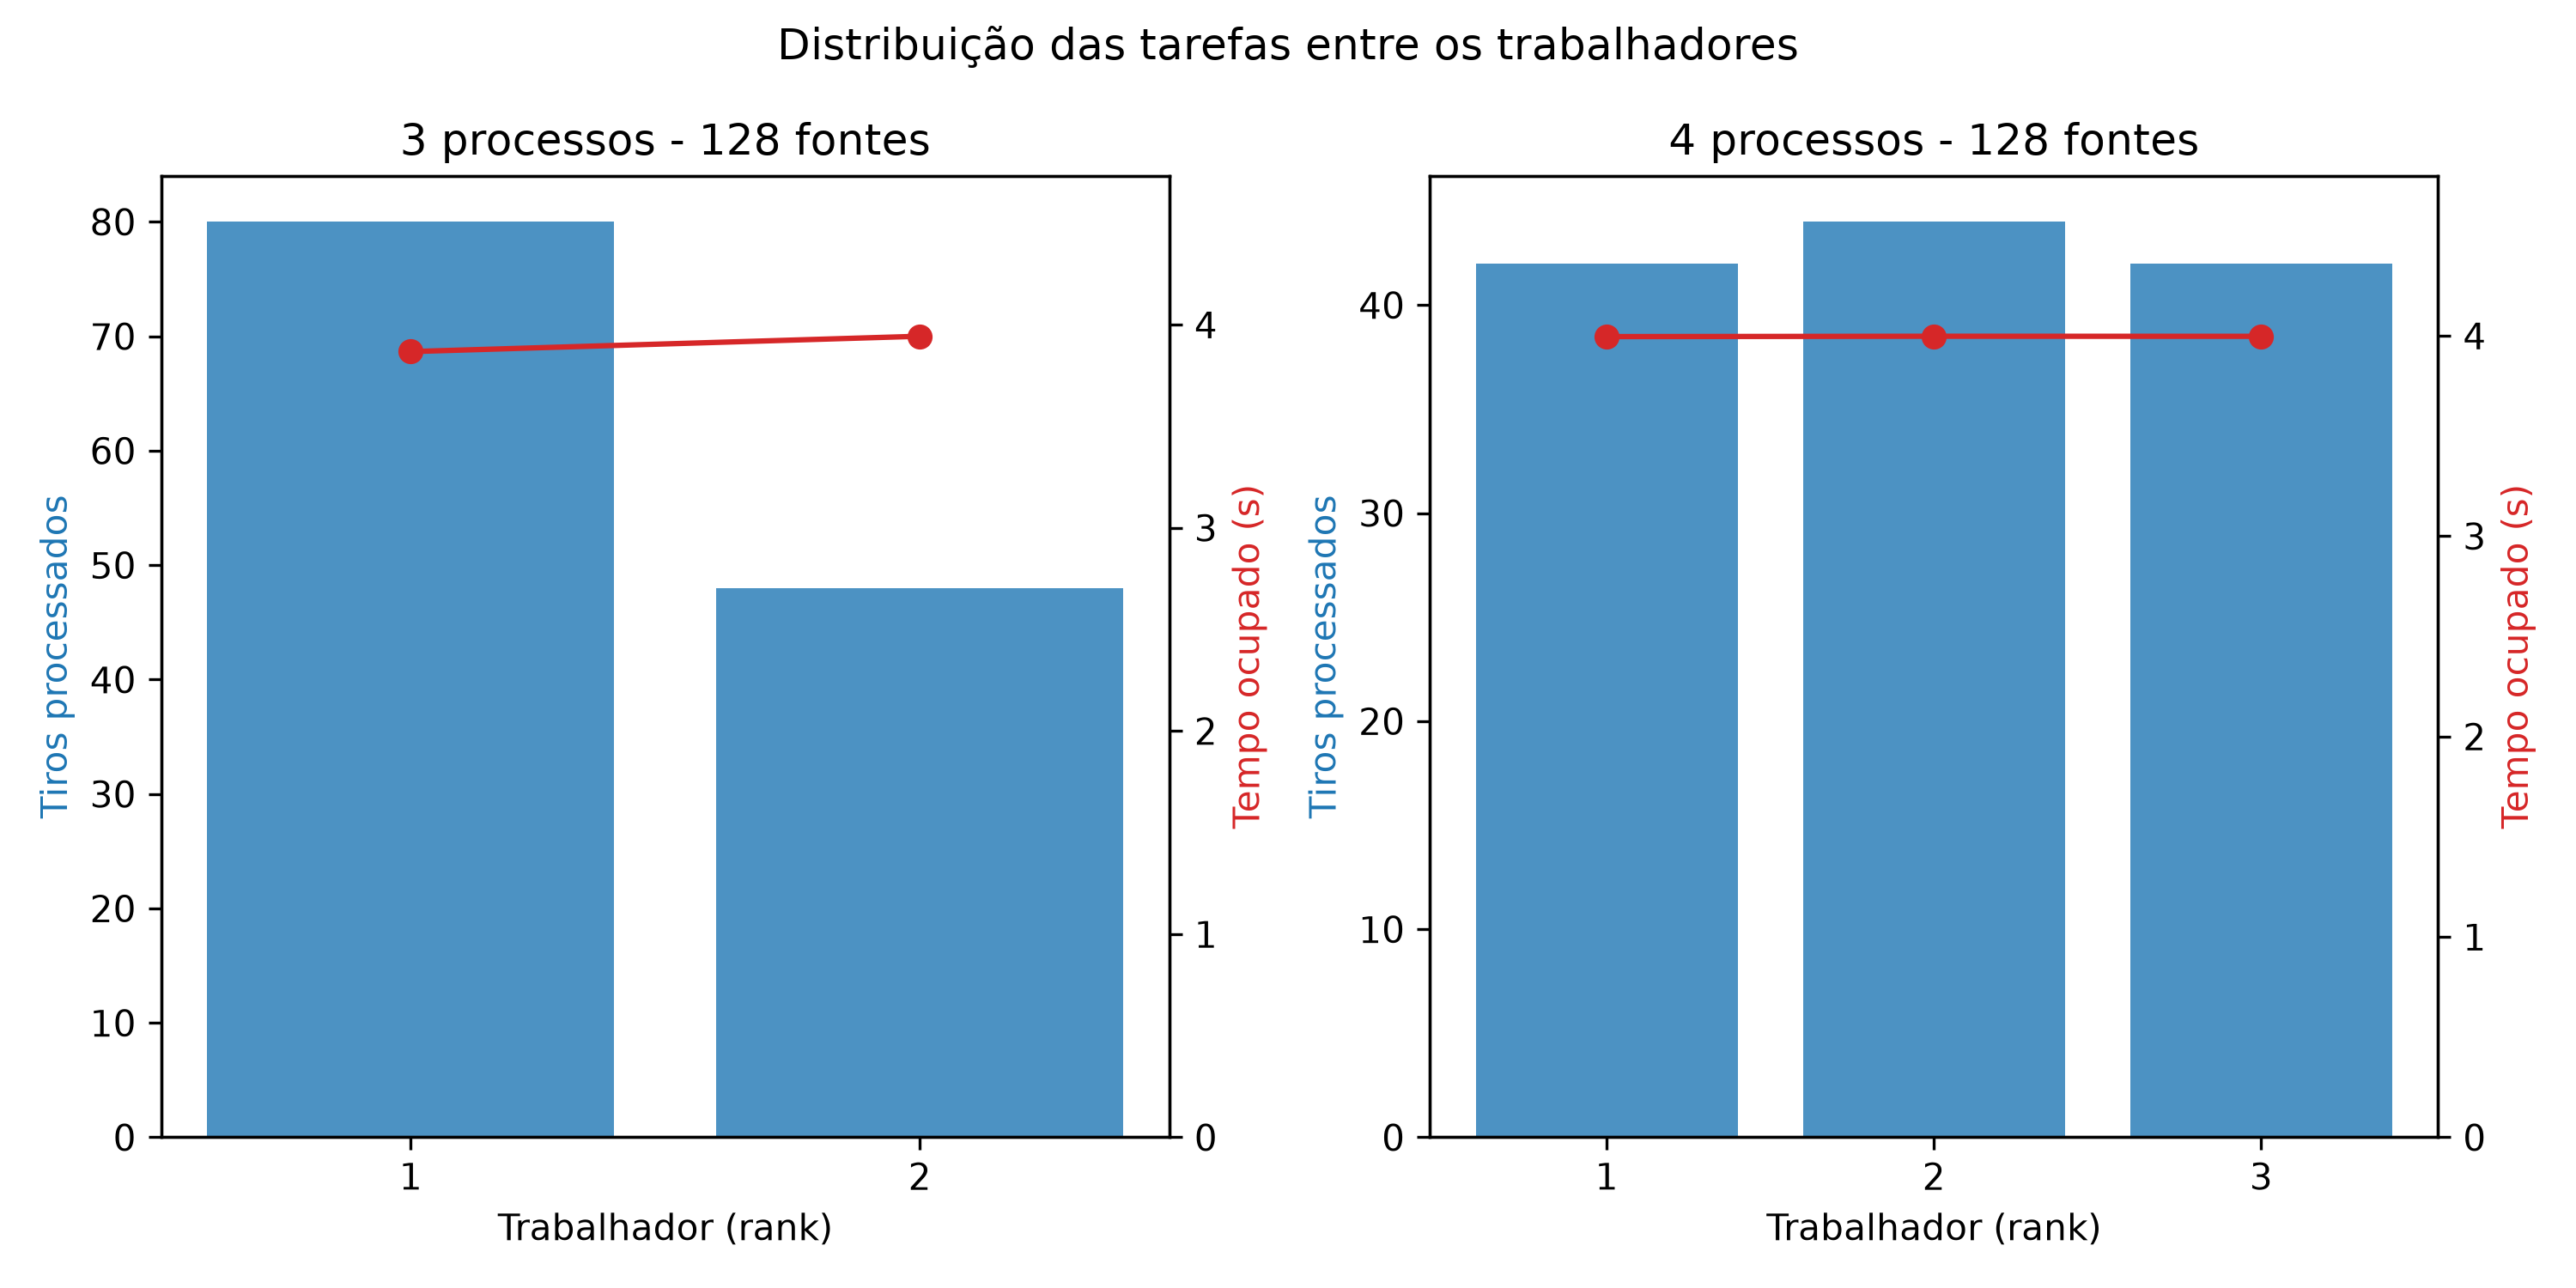
\includegraphics[width=\linewidth]{Tarefa18/tarefa18_distribuicao.png}
			\caption{Tarefa 18 -- Distribuição dinâmica das tarefas: número de tiros processados e tempo ocupado por trabalhador no maior experimento.}
		\end{figure}
		\begin{figure}[H]
			\centering
			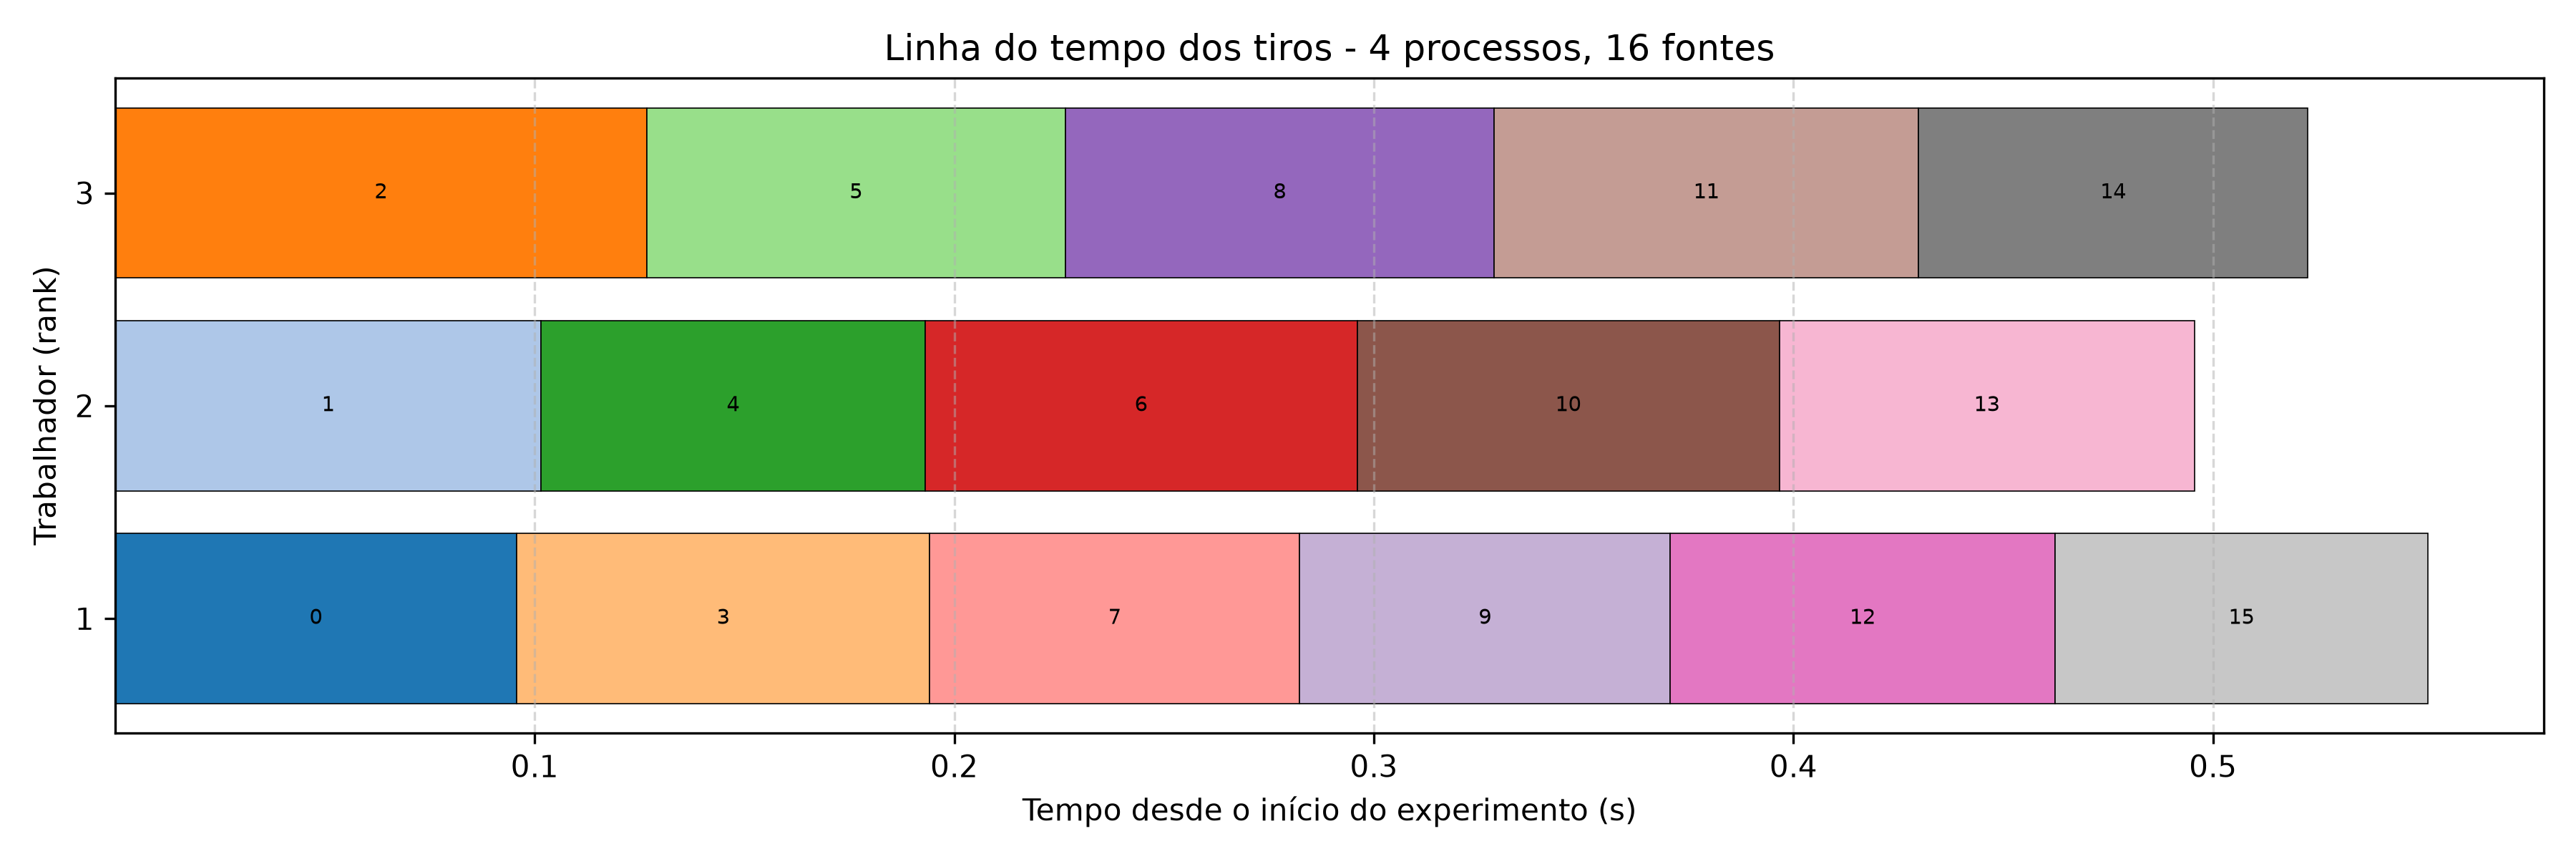
\includegraphics[width=\linewidth]{Tarefa18/tarefa18_gantt.png}
			\caption{Tarefa 18 -- Linha do tempo (diagrama de Gantt) dos tiros atribuídos a cada trabalhador pelo escalonador dinâmico.}
		\end{figure}
		\subsection{\subtTres}
		\begin{lstlisting}[language=c]
		\end{lstlisting}
		
	\newpage
		\onehalfspacing
		\section{TAREFA 19}
		\subsection{\subtUm}
		\par{Implementar um programa MPI que calcule o produto y=A*x, onde A é uma matriz M*N e x é um vetor de tamanho N.
		
		A matriz deve ser dividida por linhas entre os processos com MPI\_Scatter, o vetor x deve ser distribuído com MPI\_Bcast, e cada processo deve calcular os elementos e enviá-los de volta ao processo 0 com MPI\_Gather.
		
		Comparar os tempos com diferentes tamanhos de matriz e números de processos, executando pelo NPAD com pelo menos dois nós.}
		\subsection{\subtDois}
		\par{Texto}
		\begin{figure}[H]
			\centering
			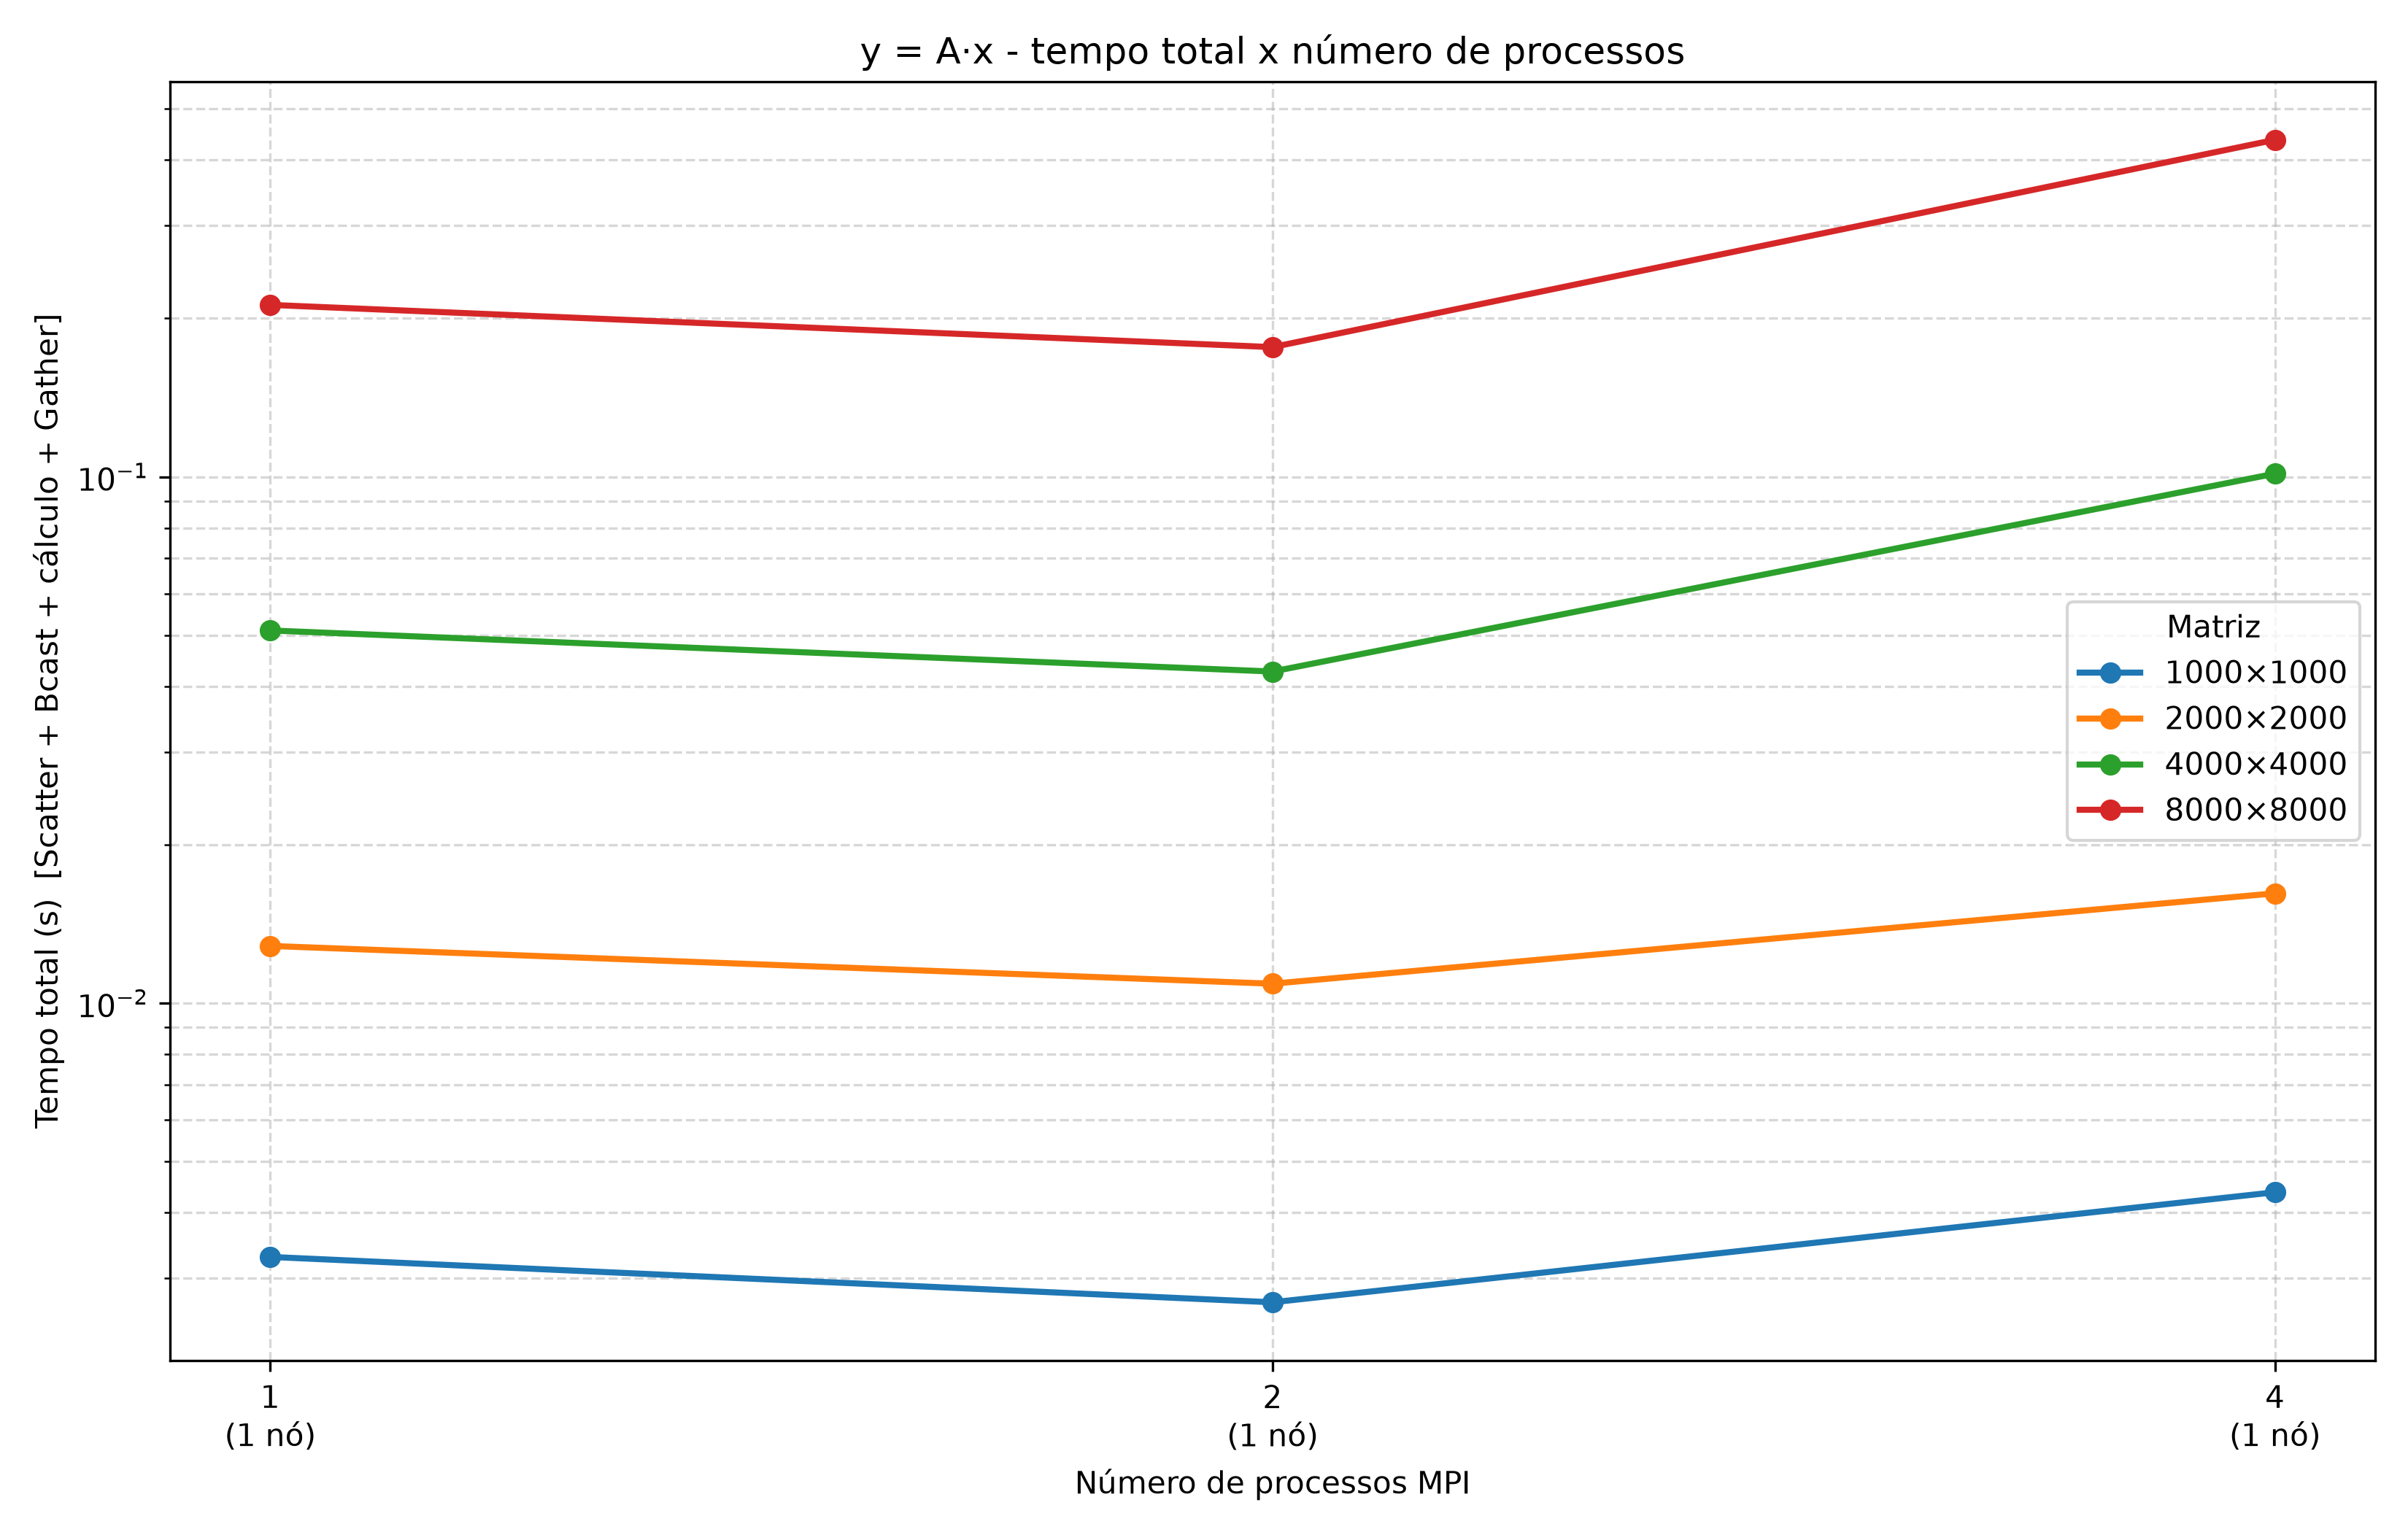
\includegraphics[width=\linewidth]{Tarefa19/tarefa19_tempo.png}
			\caption{Tarefa 19 -- Tempo total do produto $y = A \cdot x$ (\texttt{MPI\_Scatter} + \texttt{MPI\_Bcast} + cálculo + \texttt{MPI\_Gather}) em função do número de processos, para cada tamanho de matriz.}
		\end{figure}
		\begin{figure}[H]
			\centering
			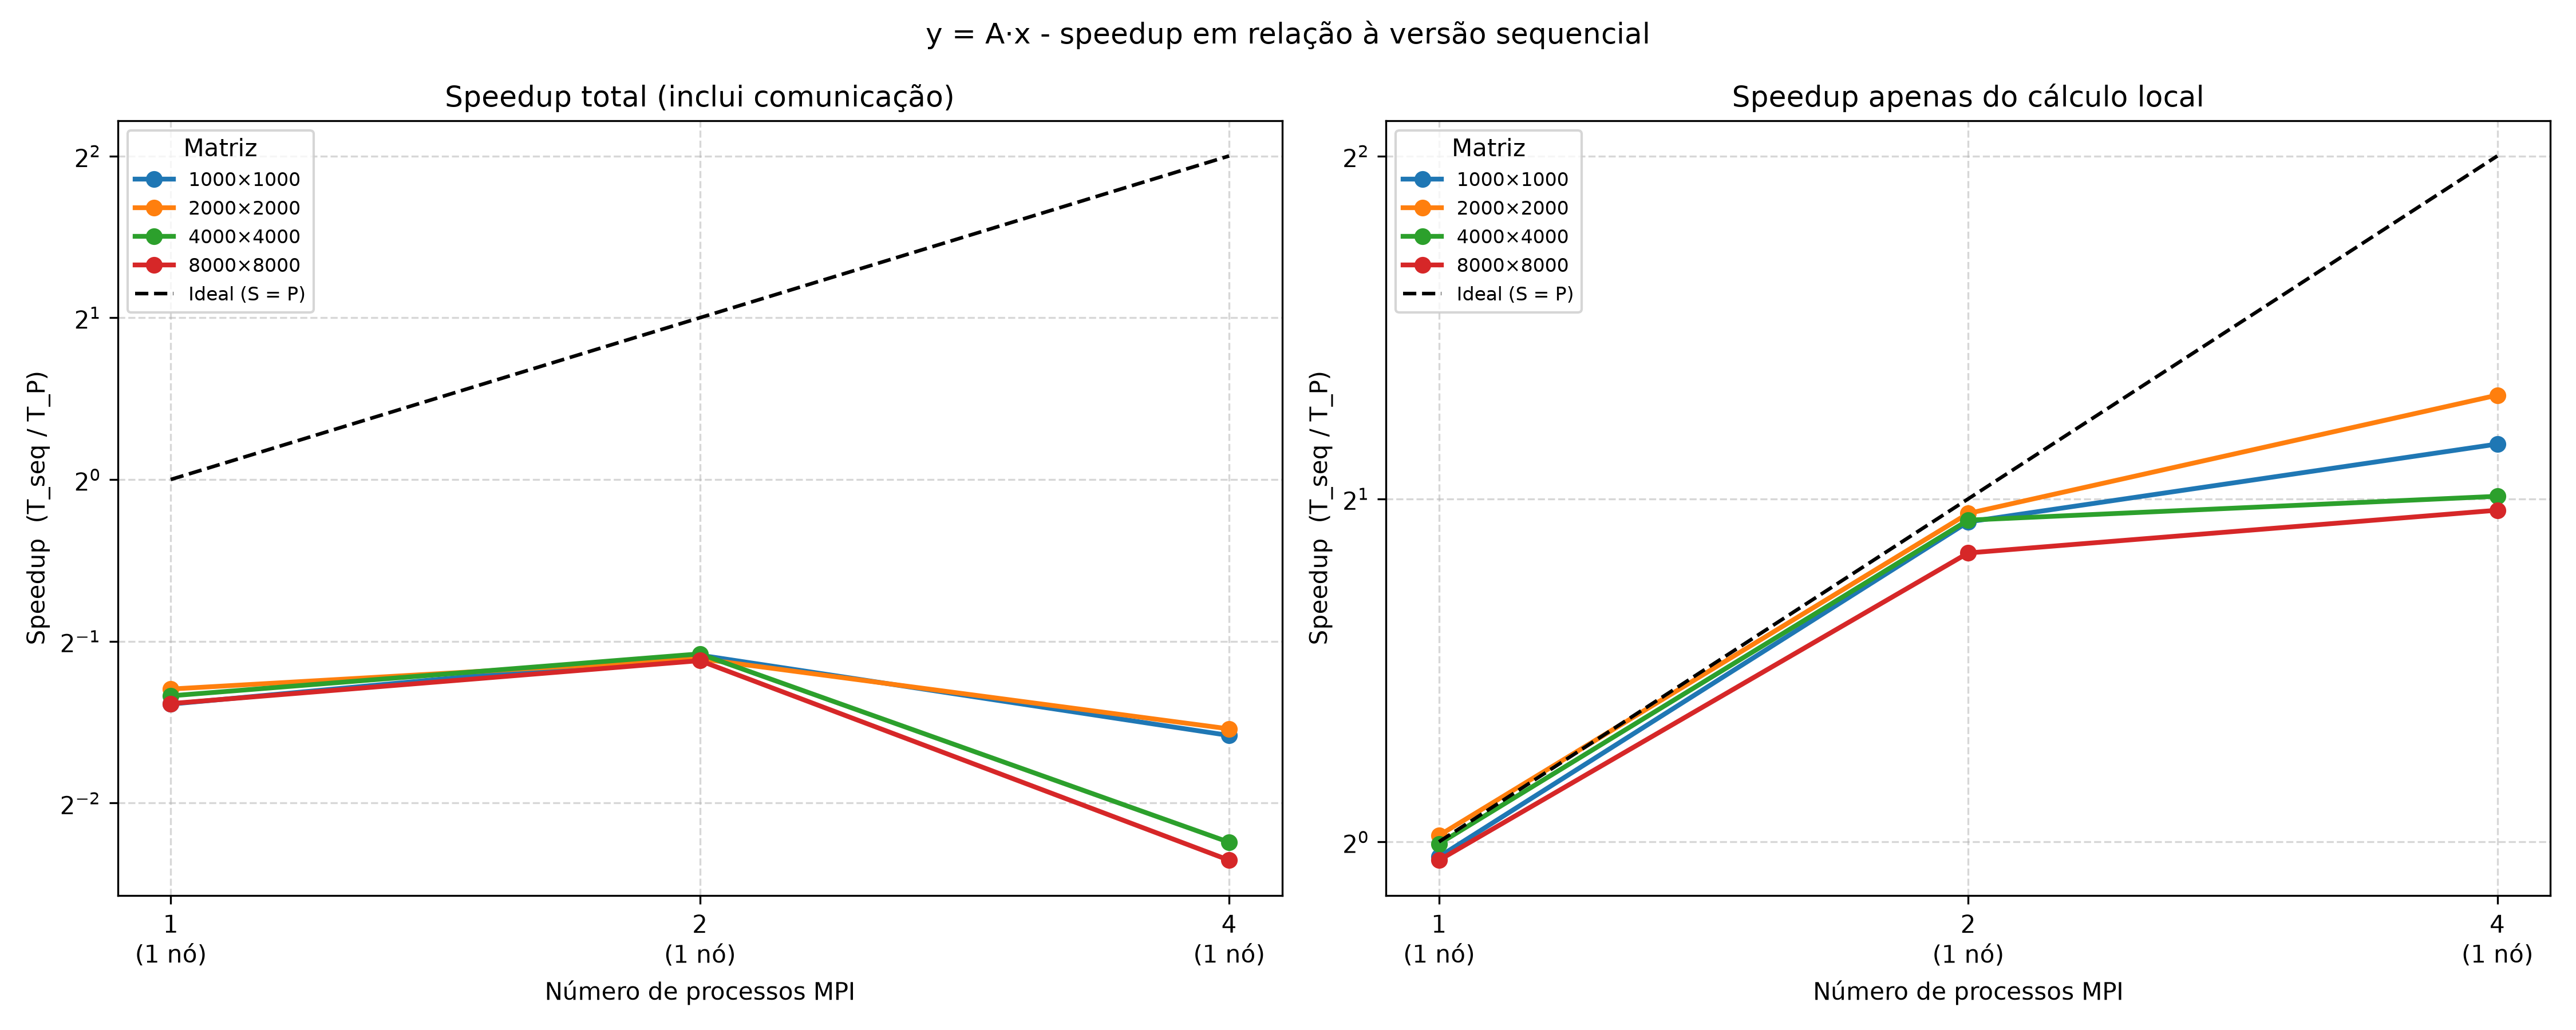
\includegraphics[width=\linewidth]{Tarefa19/tarefa19_speedup.png}
			\caption{Tarefa 19 -- \textit{Speedup} em relação à versão sequencial: à esquerda, incluindo a comunicação; à direita, apenas o cálculo local de cada processo.}
		\end{figure}
		\begin{figure}[H]
			\centering
			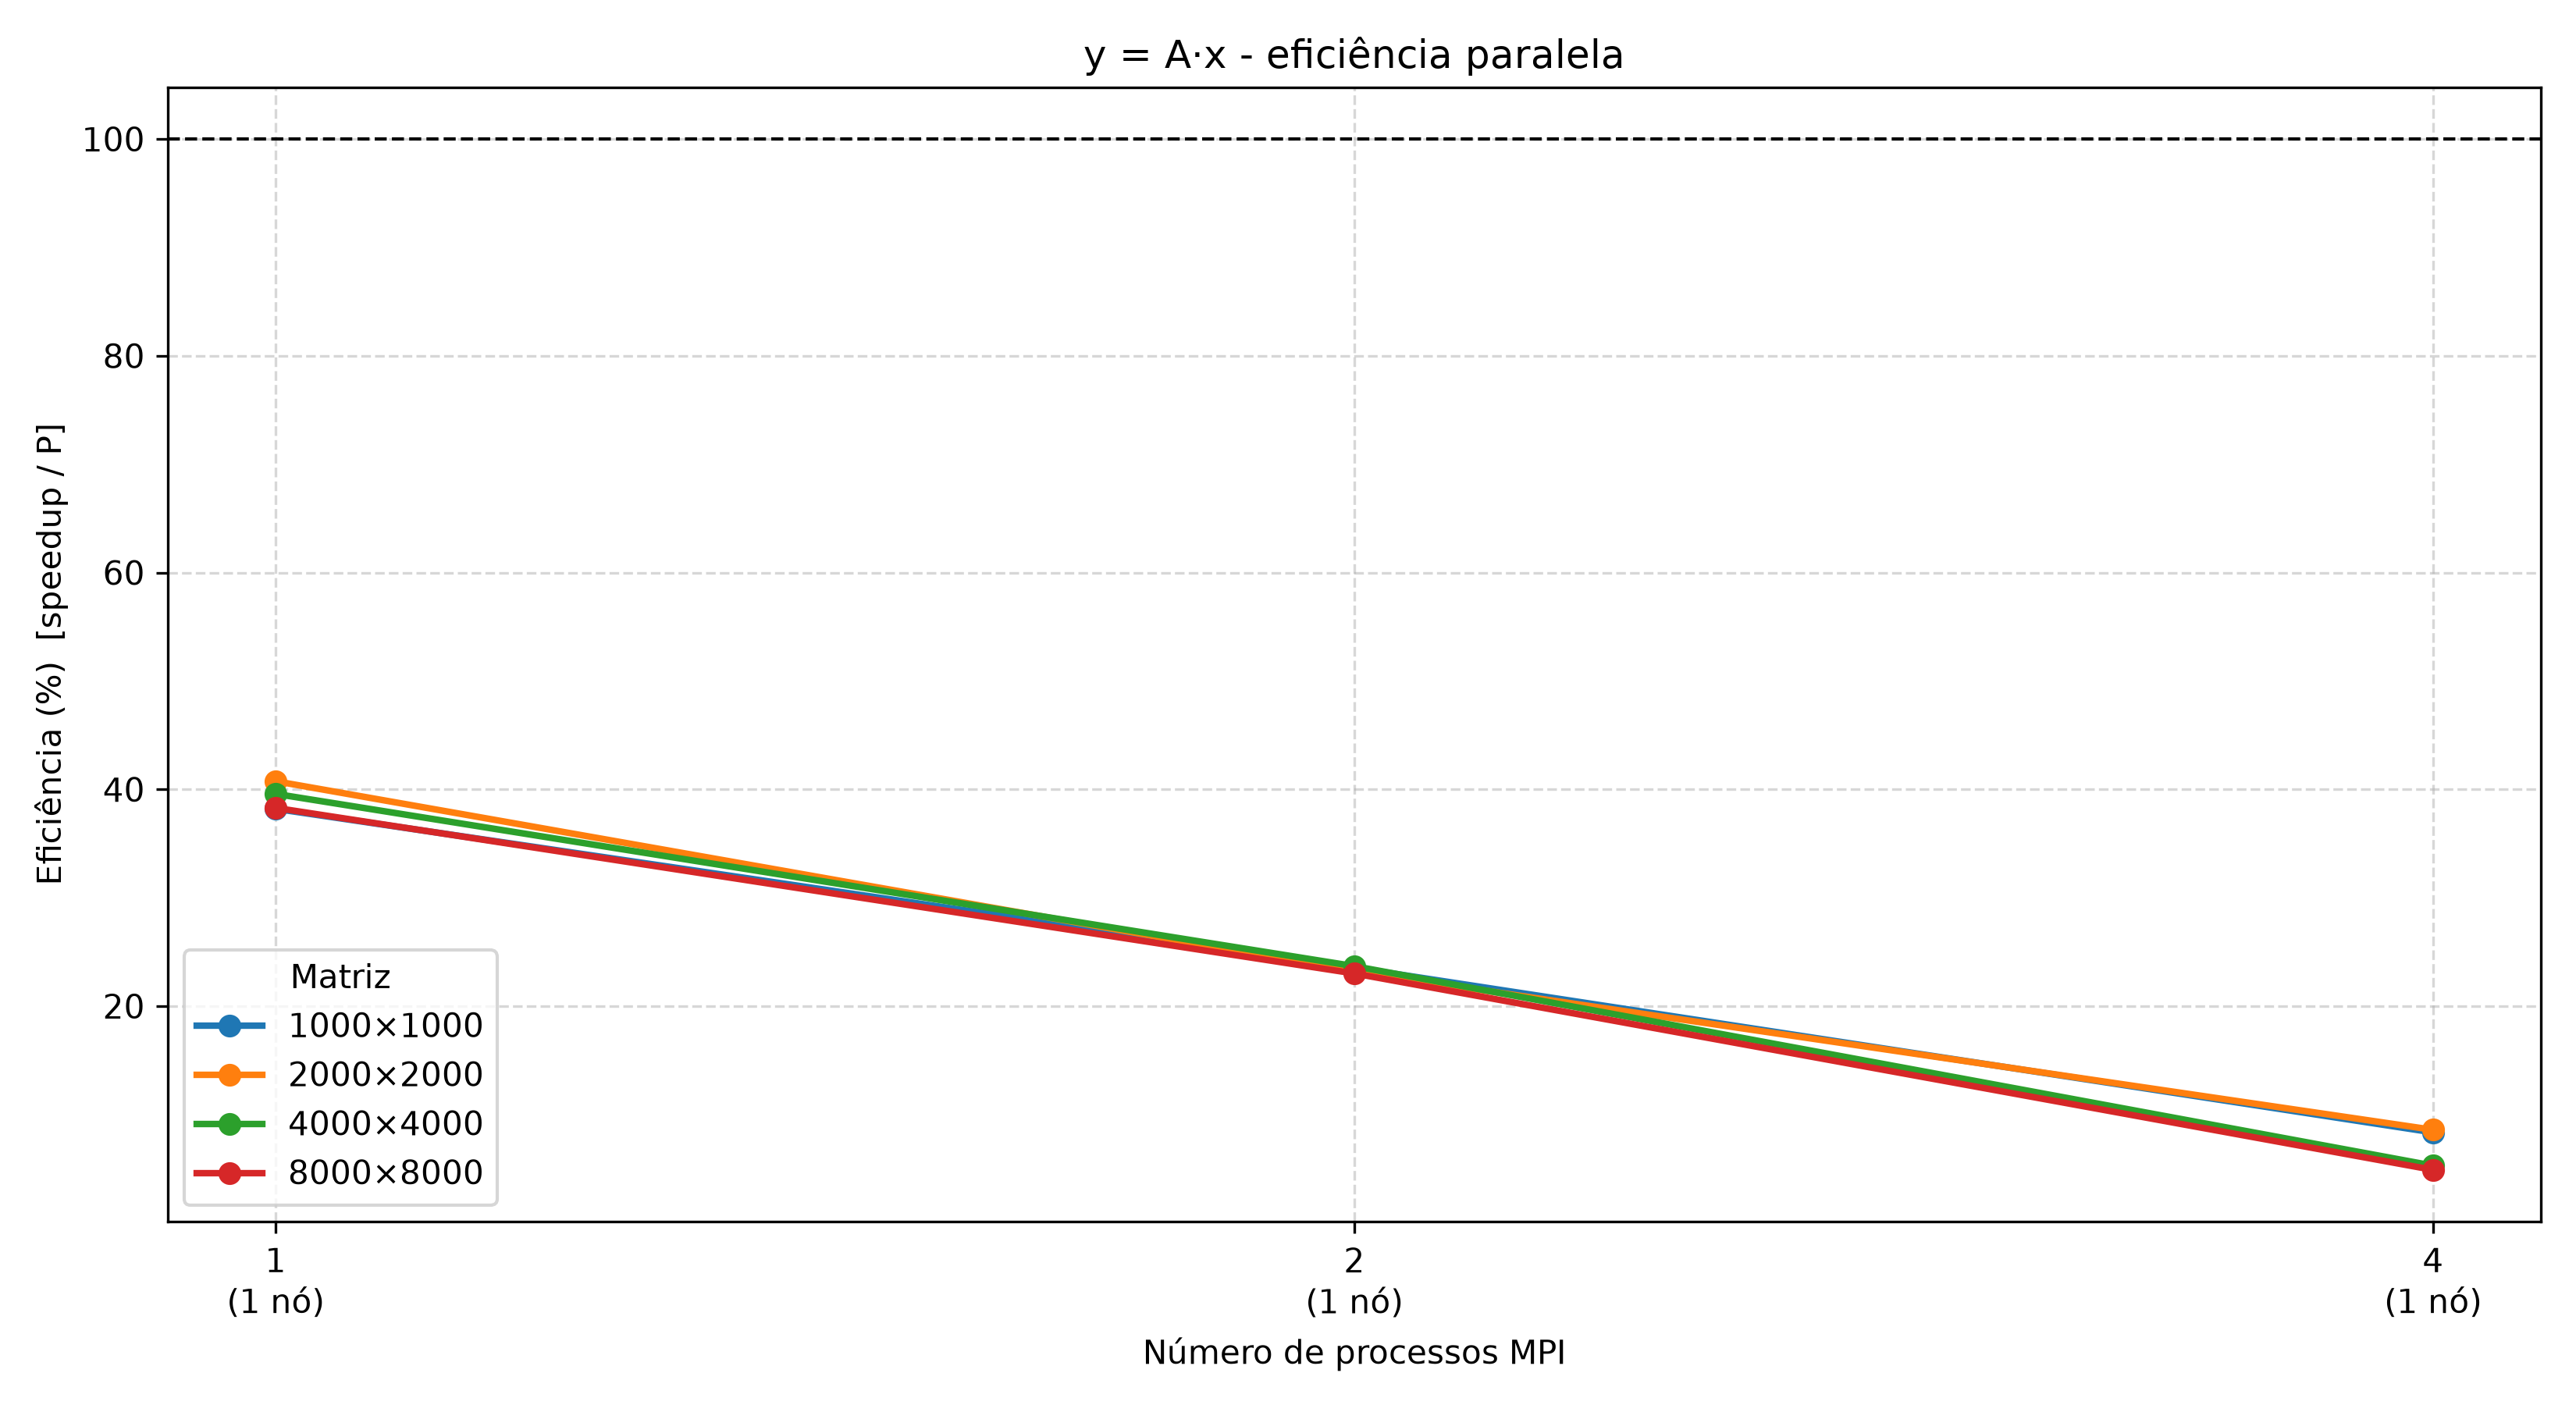
\includegraphics[width=\linewidth]{Tarefa19/tarefa19_eficiencia.png}
			\caption{Tarefa 19 -- Eficiência paralela (\textit{speedup}/$P$) em função do número de processos para cada tamanho de matriz.}
		\end{figure}
		\begin{figure}[H]
			\centering
			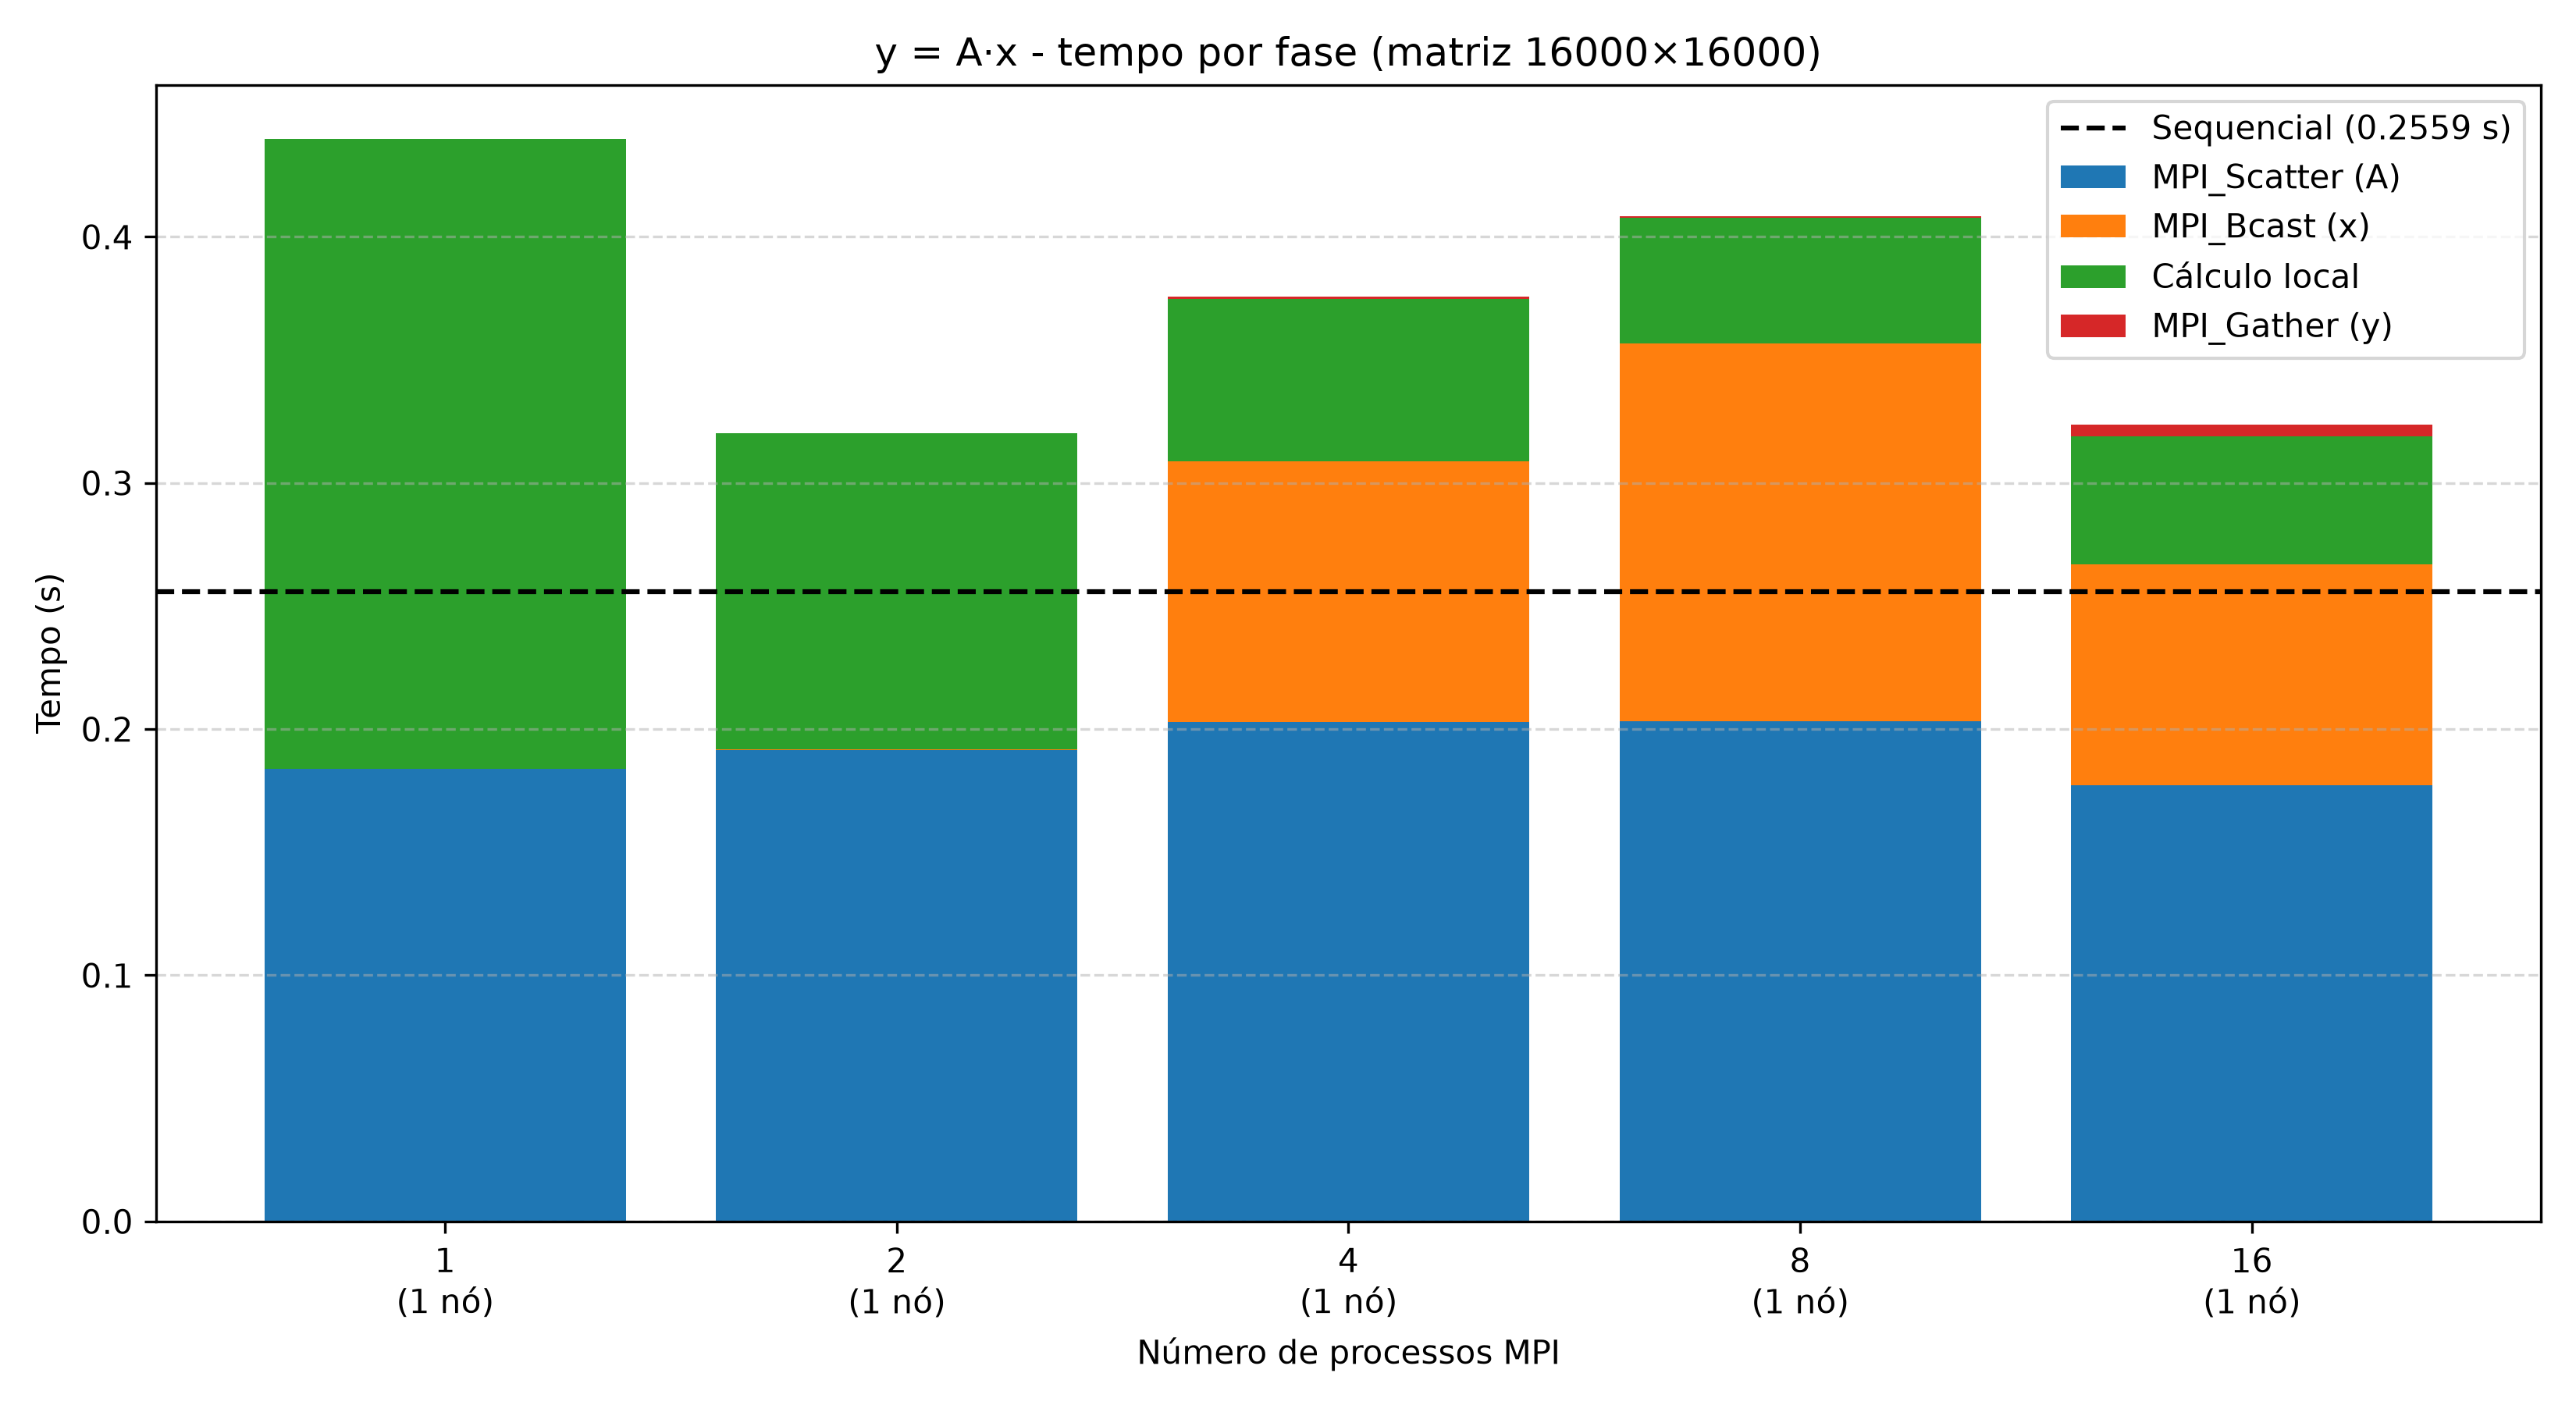
\includegraphics[width=\linewidth]{Tarefa19/tarefa19_fases.png}
			\caption{Tarefa 19 -- Tempo de cada fase (distribuição de $A$, difusão de $x$, cálculo local e coleta de $y$) para a maior matriz, em função do número de processos; a linha tracejada é o tempo sequencial.}
		\end{figure}
		\subsection{\subtTres}
		\begin{lstlisting}[language=c]
		\end{lstlisting}

	\newpage
		\onehalfspacing
		\section{TAREFA 20}
		\subsection{\subtUm}
		\par{Desenvolver um programa paralelo para calcular a integral definida de uma função utilizando o método do trapézio.
		
		O programa deve dividir o trabalho entre os processos MPI com paralelismo local, tolerância a falhas, redução global e validação do resultado.
		
		Analisar os resultados, comparando o desempenho da execução utilizando CPU e GPU, avaliando o impacto da comunicação entre os nós no tempo total de execução.}
		\subsection{\subtDois}
		\par{Texto}
		\begin{figure}[H]
			\centering
			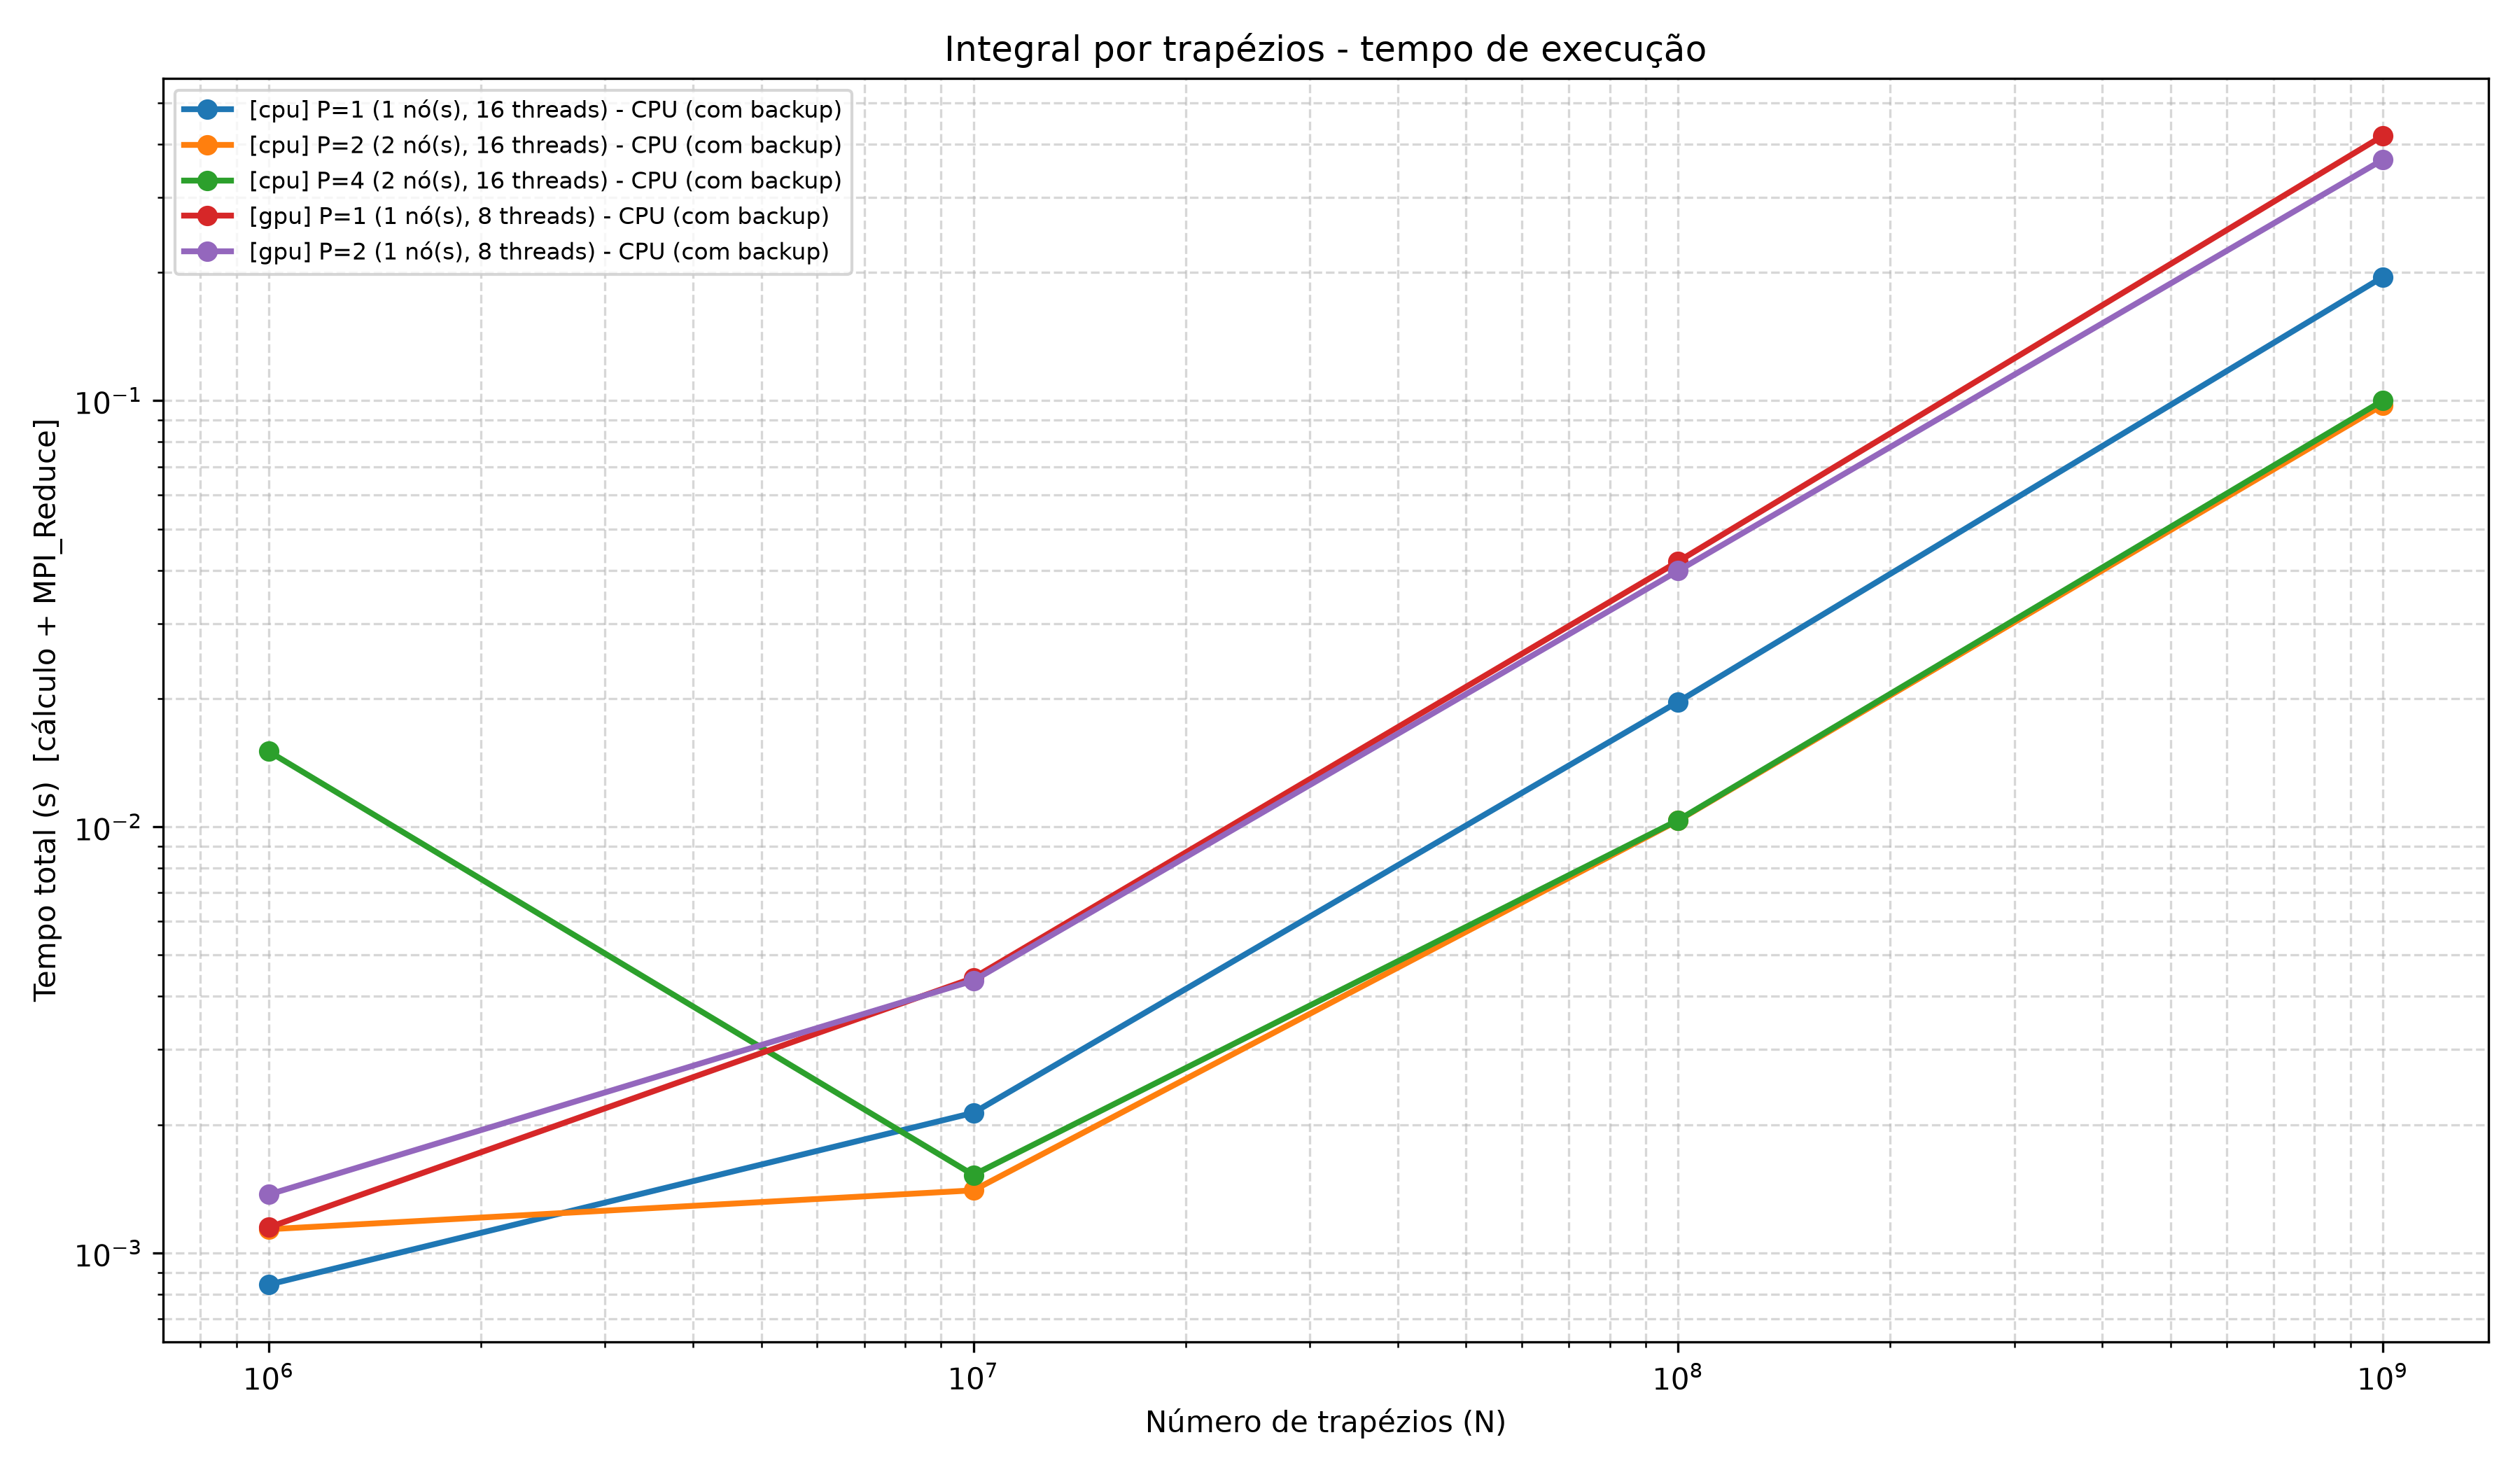
\includegraphics[width=\linewidth]{Tarefa20/tarefa20_tempo.png}
			\caption{Tarefa 20 -- Tempo total do cálculo da integral pelo método dos trapézios em função do número de trapézios, para cada configuração de processos MPI, em CPU e GPU.}
		\end{figure}
		\begin{figure}[H]
			\centering
			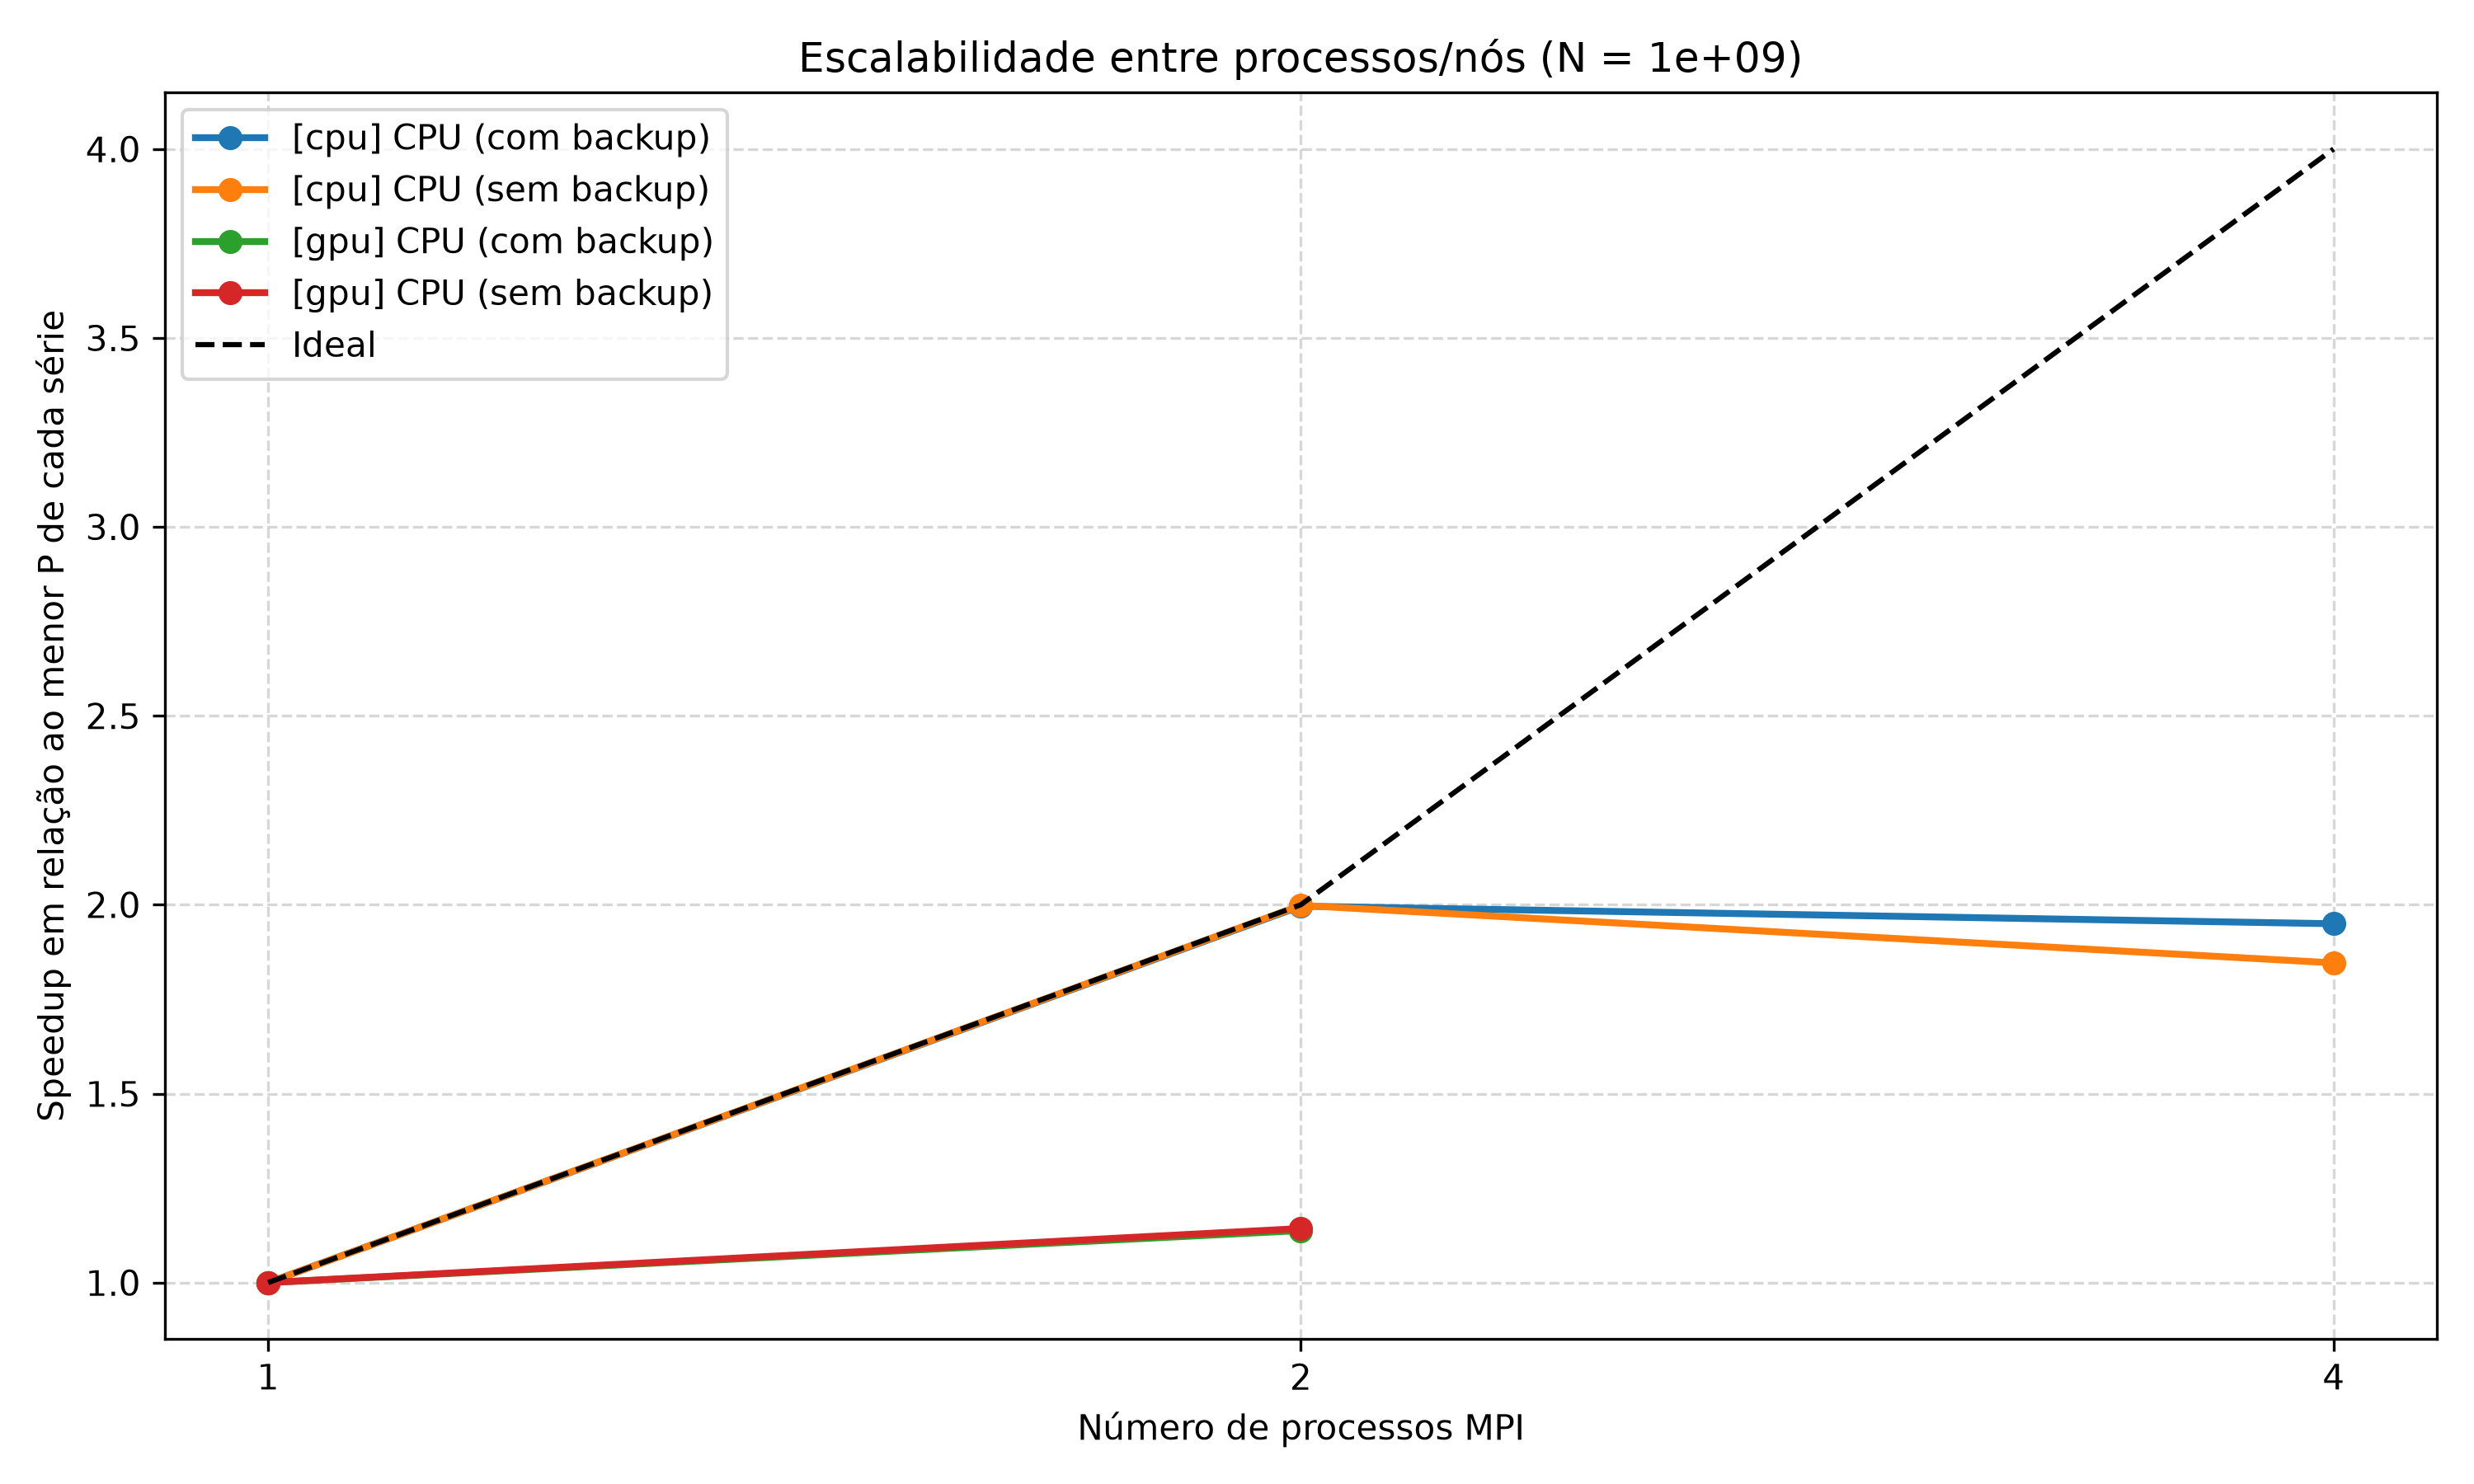
\includegraphics[width=\linewidth]{Tarefa20/tarefa20_escala.png}
			\caption{Tarefa 20 -- \textit{Speedup} em função do número de processos MPI para o maior número de trapézios, nos modos com e sem envio do backup ao vizinho.}
		\end{figure}
		\begin{figure}[H]
			\centering
			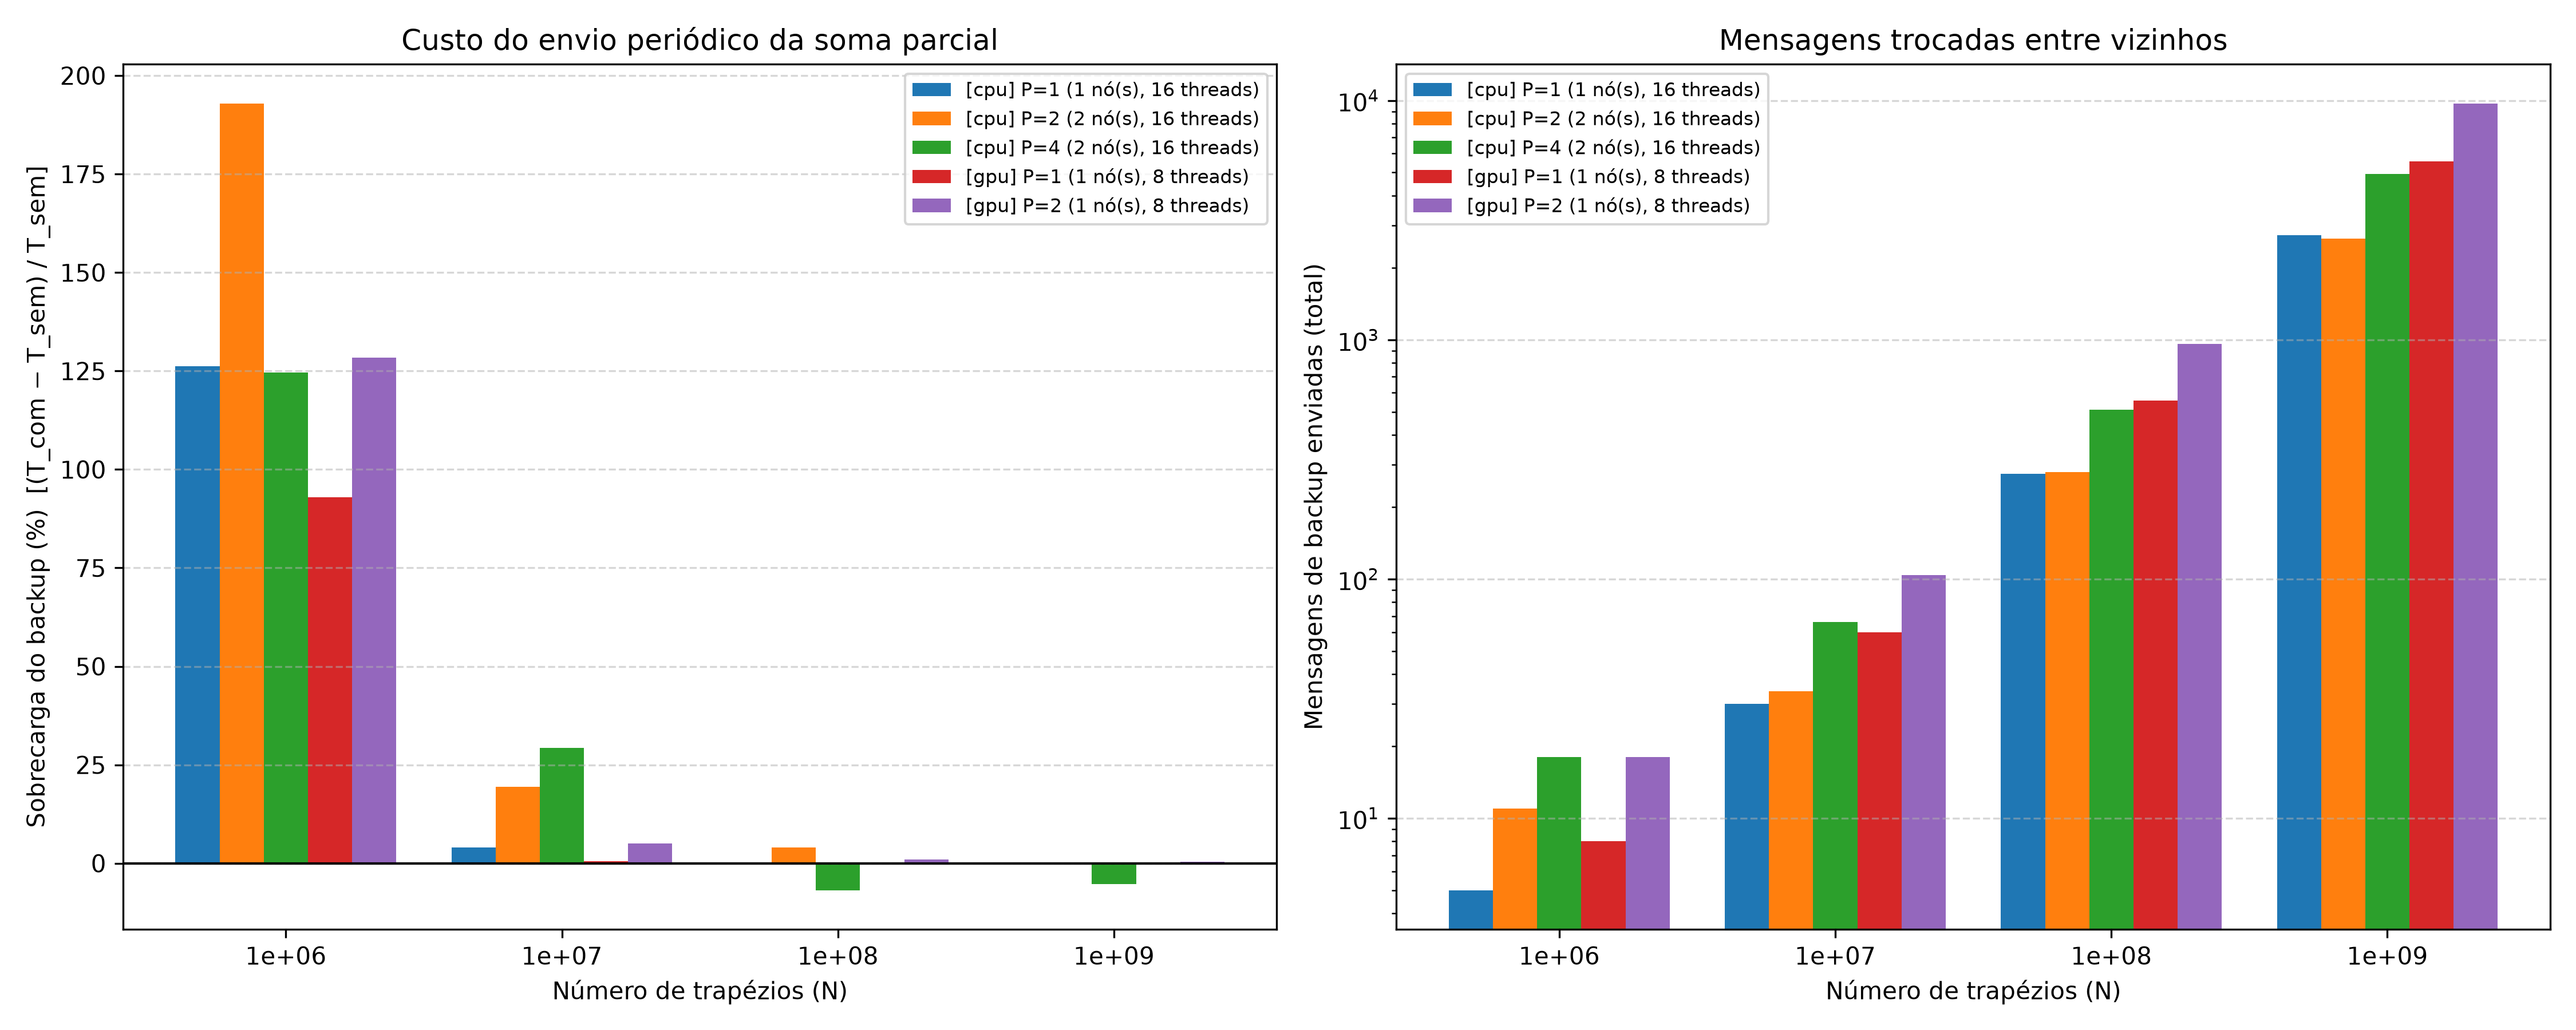
\includegraphics[width=\linewidth]{Tarefa20/tarefa20_comunicacao.png}
			\caption{Tarefa 20 -- Impacto da tolerância a falhas: sobrecarga do envio periódico da soma parcial ao processo vizinho e número de mensagens de backup trocadas.}
		\end{figure}
		\begin{figure}[H]
			\centering
			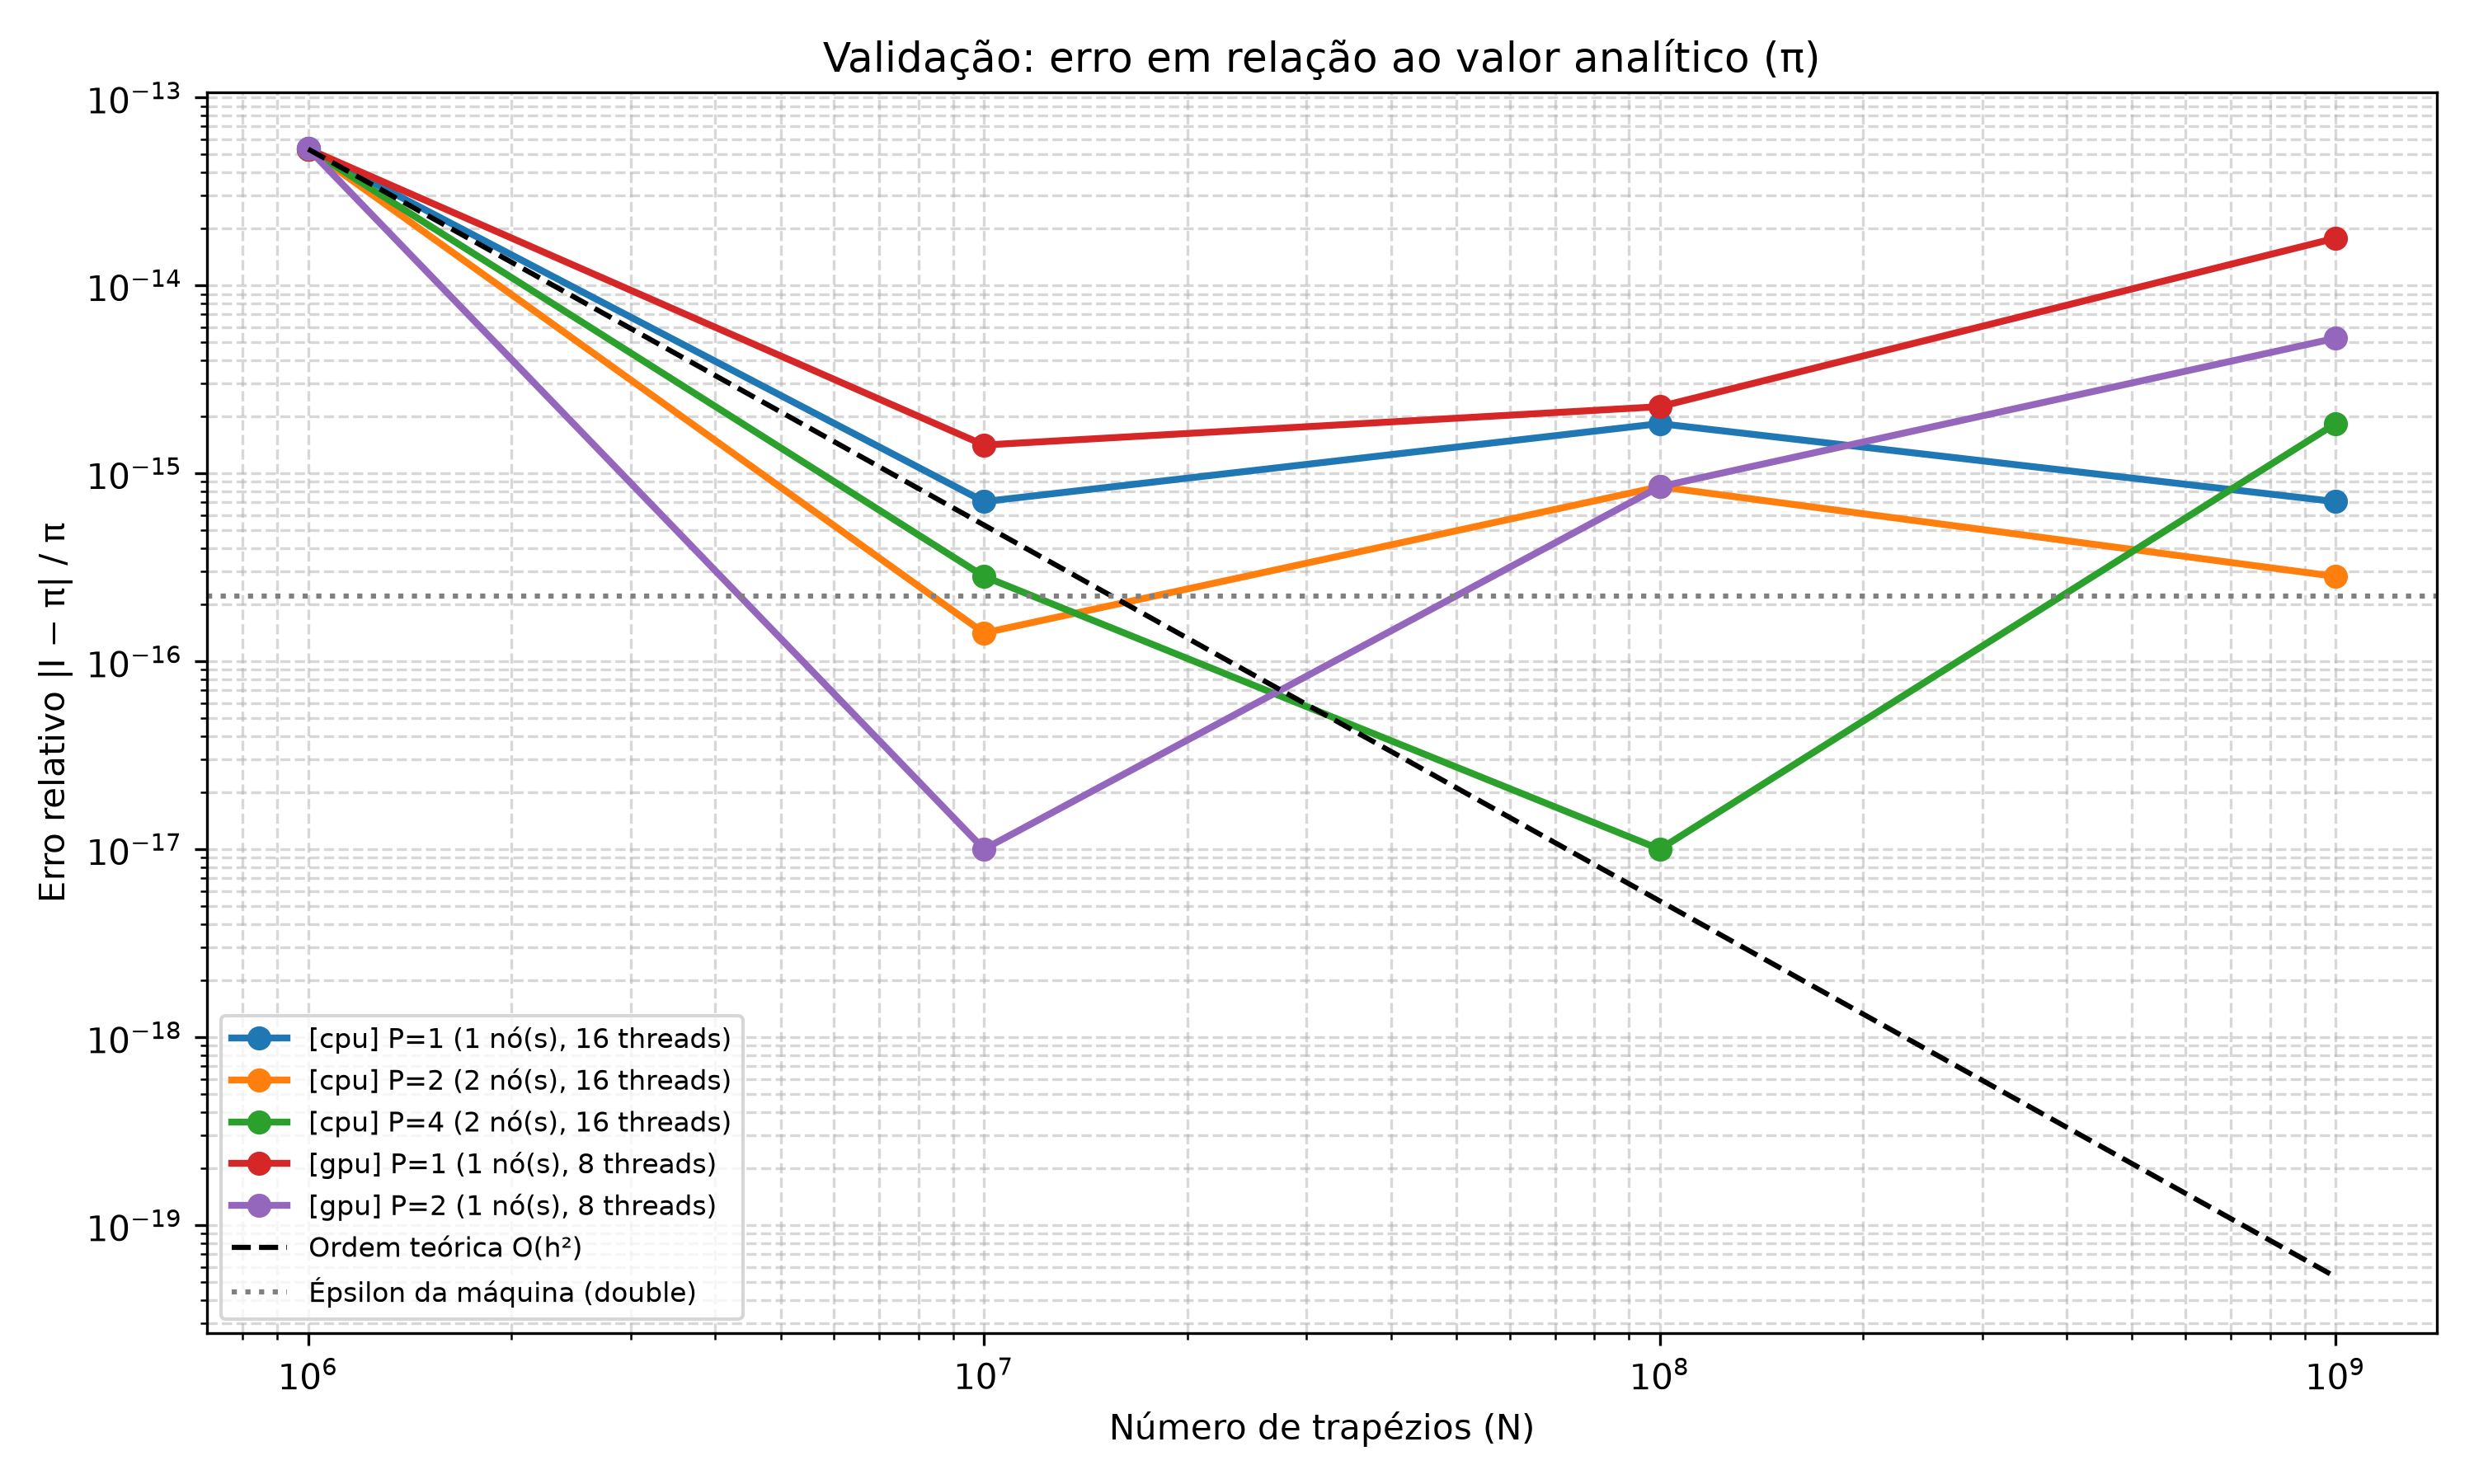
\includegraphics[width=\linewidth]{Tarefa20/tarefa20_erro.png}
			\caption{Tarefa 20 -- Erro relativo da integral em relação ao valor analítico ($\pi$) em função do número de trapézios, comparado à ordem teórica $O(h^2)$ e ao épsilon da máquina.}
		\end{figure}
		\subsection{\subtTres}
		\begin{lstlisting}[language=c]
		\end{lstlisting}


	
\end{document}
